\section{Taking a slice: diabetic patient analysis}
\graphicspath{{./img/diabetes/}}

\begin{frame}
    \frametitle{General methods for slice analysis}
    \textbf{Too wordy?}
    Given some slice of the data, we want to:
    \begin{itemize}
        \item Examine cost variations and general surface-level statistics
        \item Determine components and variable relationships of interest
        \item Consider the relative `cost' of the patients in this slice
        \item Contrast this against its complement and the general dataset
    \end{itemize}
\end{frame}

\begin{frame}
    \frametitle{Diabetic patient analysis}

    This is a known area of interest to the health board.

    \vspace{10pt}
    Diabetic patients make up 10.8\% of all the episodes in the dataset, and
    roughly 8.7\% of the unique patients in the dataset.

    \vspace{10pt}
    Here we consider patients to be `diabetic' if they have diabetes flagged as
    either a primary or secondary condition in their episode.
\end{frame}

\documentclass{beamer}

\usepackage{graphicx}

\title{An exploratory analysis of patient episode data}
\author{Henry Wilde}
\institute{Cardiff University School of Mathematics}

\usetheme{Hannover}
\usecolortheme{seahorse}
\begin{document}

\begin{frame}
\titlepage%
\end{frame}

\begin{frame}
\frametitle{Outline}
\tableofcontents
\end{frame}

\section{Motivation}

\begin{frame}
\frametitle{Motivation}

\begin{itemize}
    \item Observe and understand cost variation
    \item Identify important slices in the data
    \item Develop methods for examining slices of the data
    \item Analyse their impact on costs and resource consumption
\end{itemize}
\end{frame}

\section{Getting to know the data}

\subsection{Structure and origin}
\begin{frame}
    \frametitle{Structure and origin}

    \pause%
    All data is provided by the Cwm Taf University Health Board.
    \vspace{10pt}

    \pause%
    We have:
    \begin{itemize}
        \item 2,447,299 patient episodes
        \item 1,946,545 patient spells
        \item 865,421 individual patients
    \end{itemize}
    \vspace{10pt}

    \pause%
    Each row is made up of roughly 250 attributes, including:
    \begin{itemize}
        \pause%
        \item personal identifiers and demographic information
        \pause%
        \item condition and treatment indicators (HRG, OPCS4, ICD10)
        \pause%
        \item other clinical references
        \pause%
        \item cost components
    \end{itemize}
\end{frame}

\subsection{Summative analysis}
\begin{frame}
    \frametitle{Summative analysis}

    \begin{itemize}
        \pause%
        \item Our data is skewed towards low-cost, short-stay episodes
        \pause%
        \item This extends to the spell level with largely one or two-time
            visits from patients
        \pause%
        \item Long and heavy tails are present in our costs and lengths of stay
    \end{itemize}
\end{frame}

\begin{frame}
    \frametitle{Number of spells}

    \begin{figure}
        \begin{minipage}{\linewidth}
            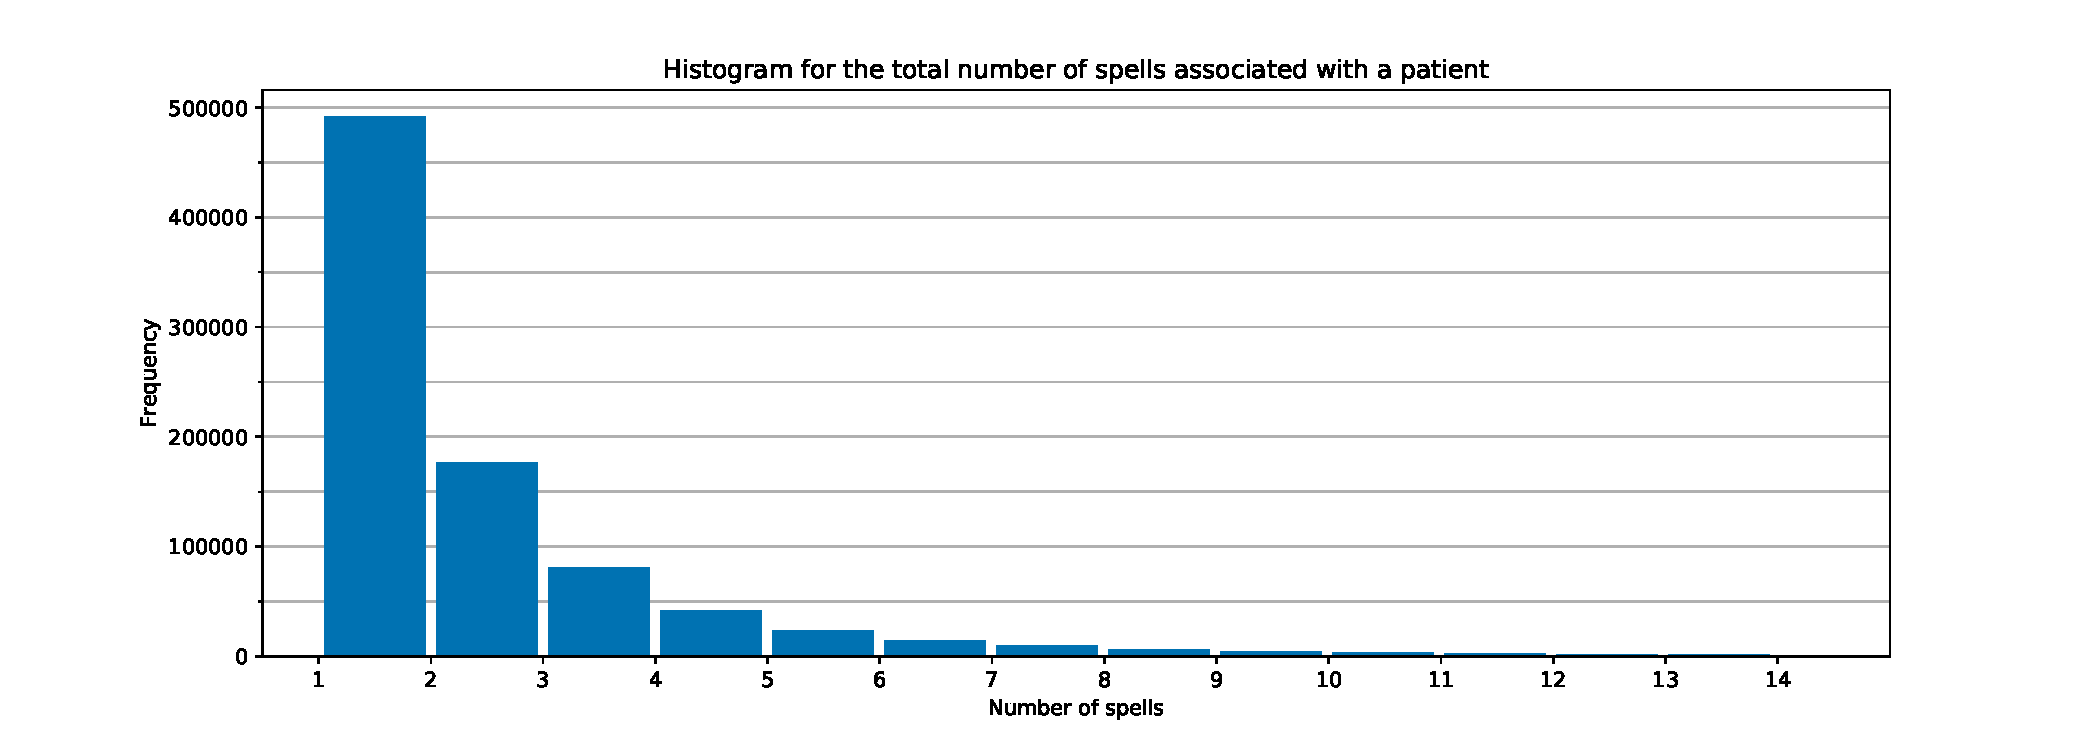
\includegraphics[width=\linewidth]{./img/no_spells_freq_hist.pdf}
        \end{minipage}
        \begin{minipage}{\linewidth}
            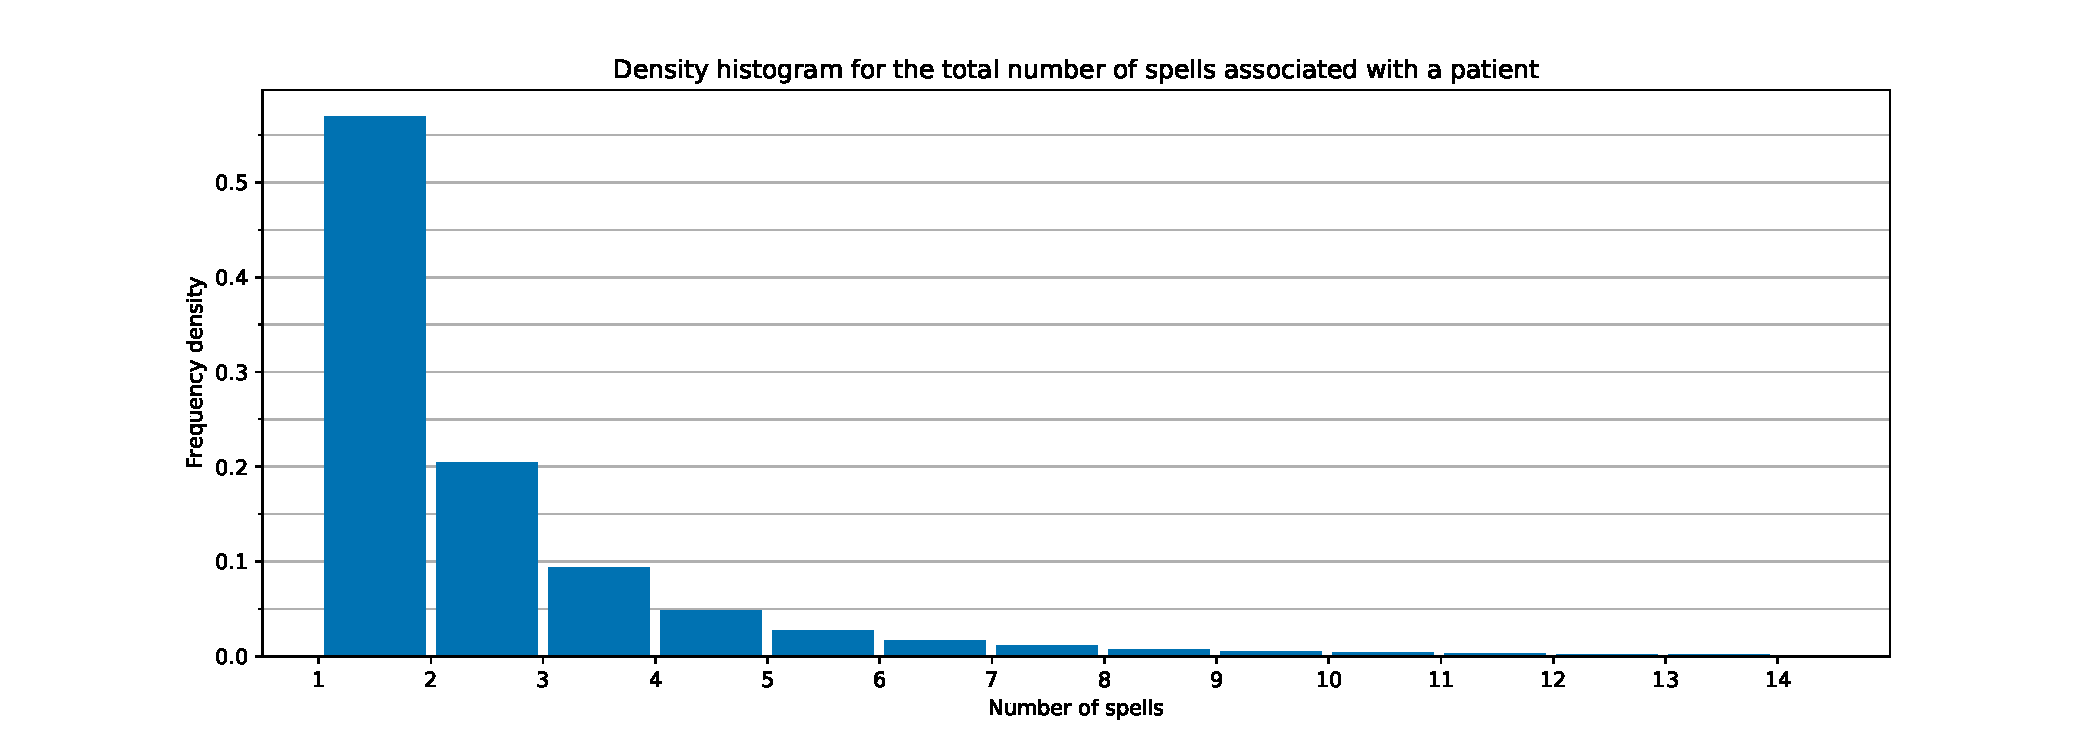
\includegraphics[width=\linewidth]{./img/no_spells_density_hist.pdf}
        \end{minipage}
    \end{figure}
\end{frame}

\begin{frame}
    \frametitle{Length of stay (spell-wise)}

    \begin{figure}
        \begin{minipage}{\linewidth}
            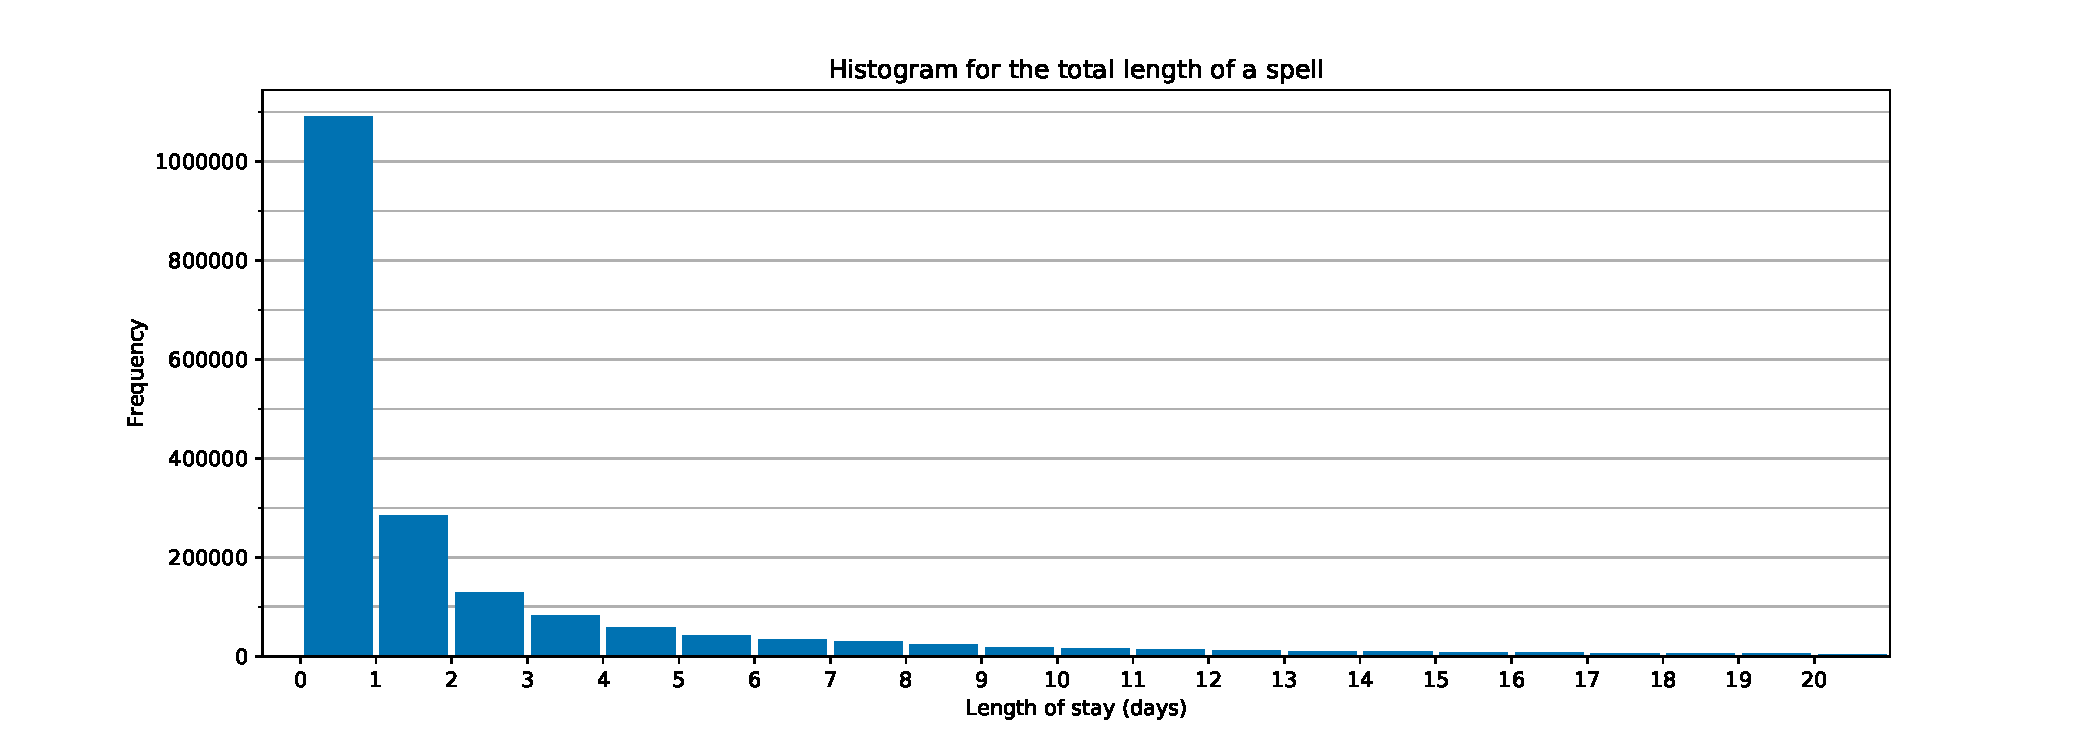
\includegraphics[width=\linewidth]{./img/LOS_freq_hist.pdf}
        \end{minipage}
        \begin{minipage}{\linewidth}
            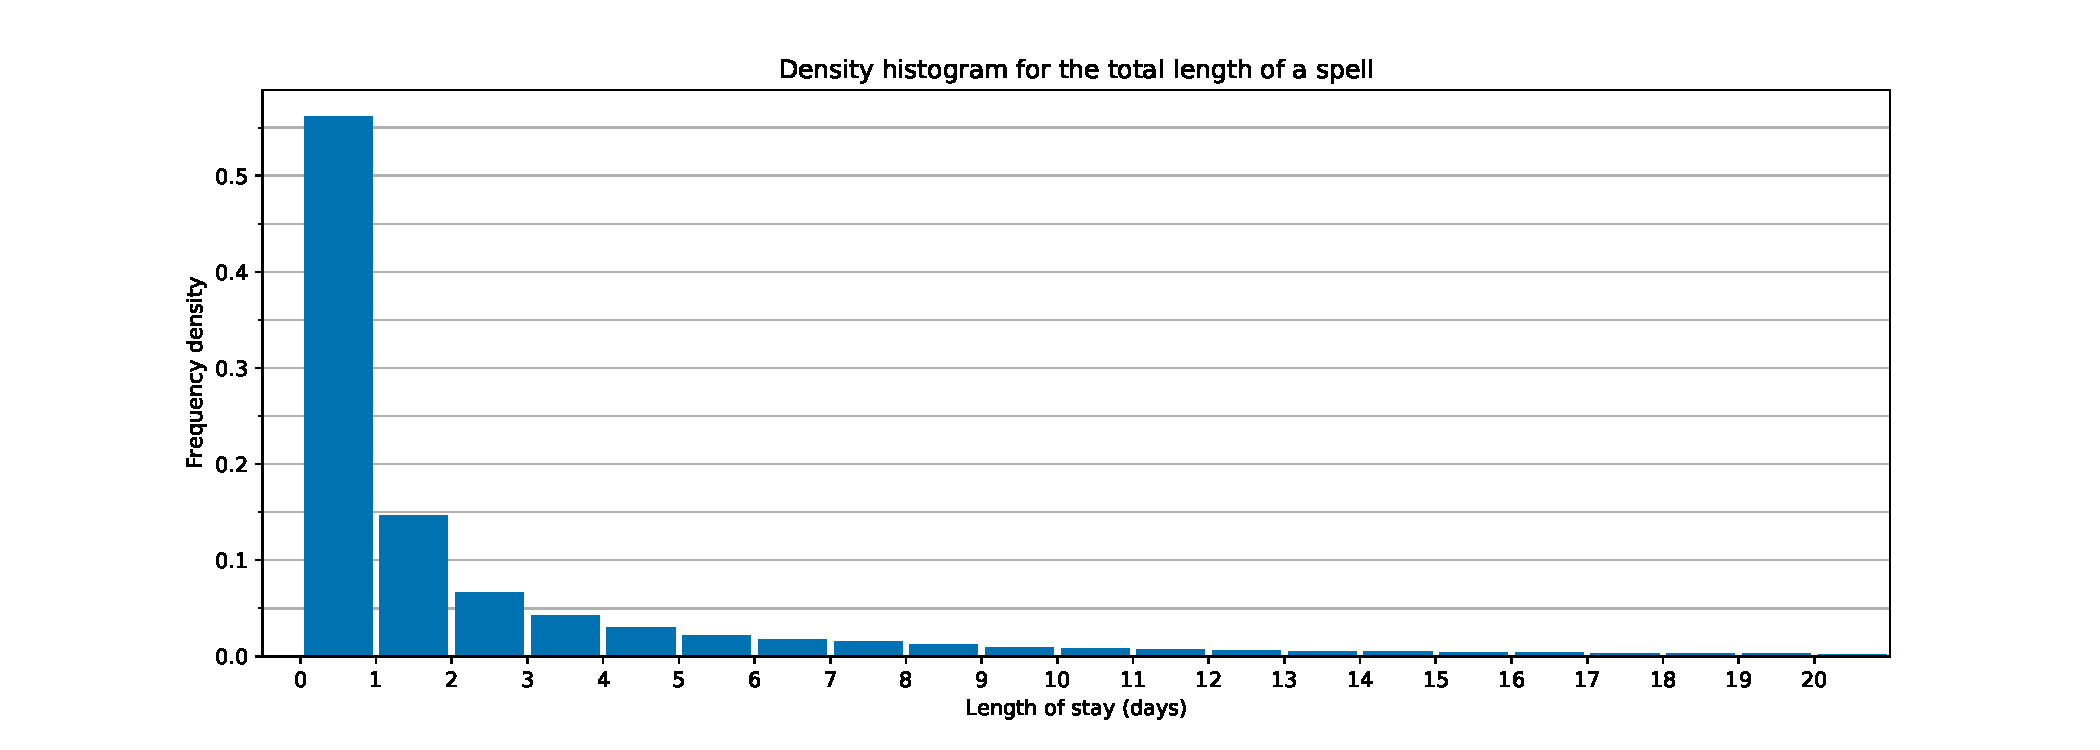
\includegraphics[width=\linewidth]{./img/LOS_density_hist.pdf}
        \end{minipage}
    \end{figure}
\end{frame}

\begin{frame}
    \frametitle{Net cost}

    \begin{figure}
        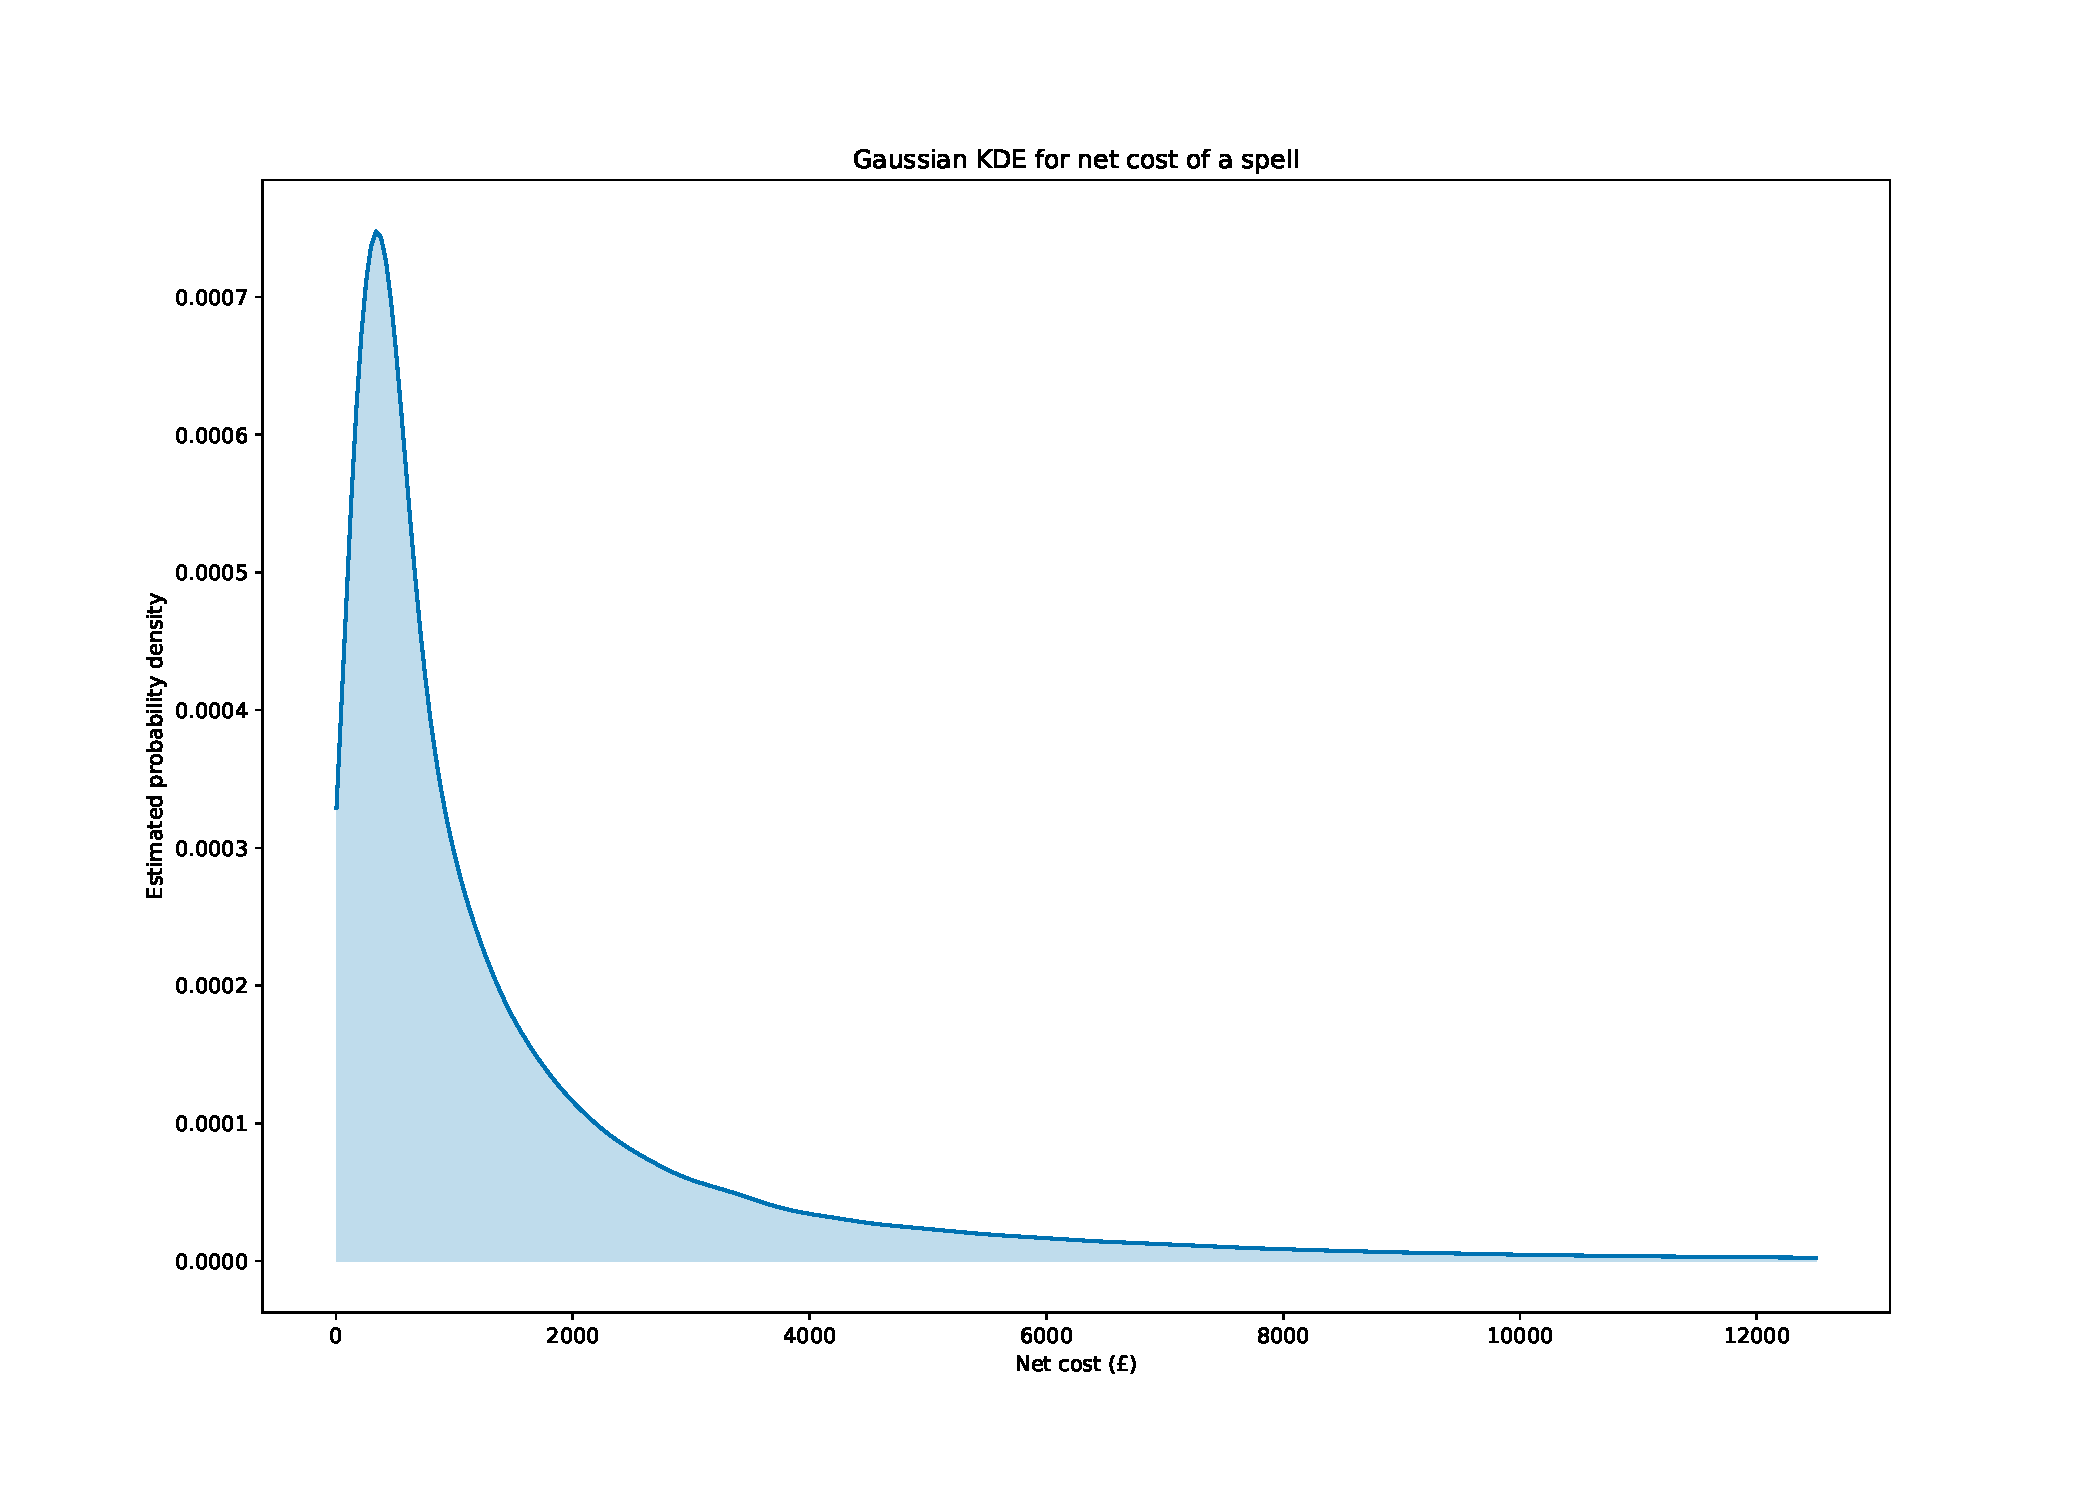
\includegraphics[width=\linewidth]{./img/netcost_kde.pdf}
    \end{figure}
\end{frame}

\begin{frame}
    \frametitle{Summative analysis}

    Other areas of interest to us are:
    \begin{itemize}
        \item Other clinical measures
        \item Demographic variables
        \item Interactions between variables
    \end{itemize}
\end{frame}

\begin{frame}
    \frametitle{Clinical variables}

    We will investigate:
    \begin{itemize}
        \item the number of diagnoses
        \item the number of procedures
    \end{itemize}

    \pause%
    These contribute to comorbidity rates and presumably costs.
\end{frame}

\begin{frame}
    \frametitle{Number of diagnoses}
   
    \begin{figure}
        \begin{minipage}{\linewidth}
            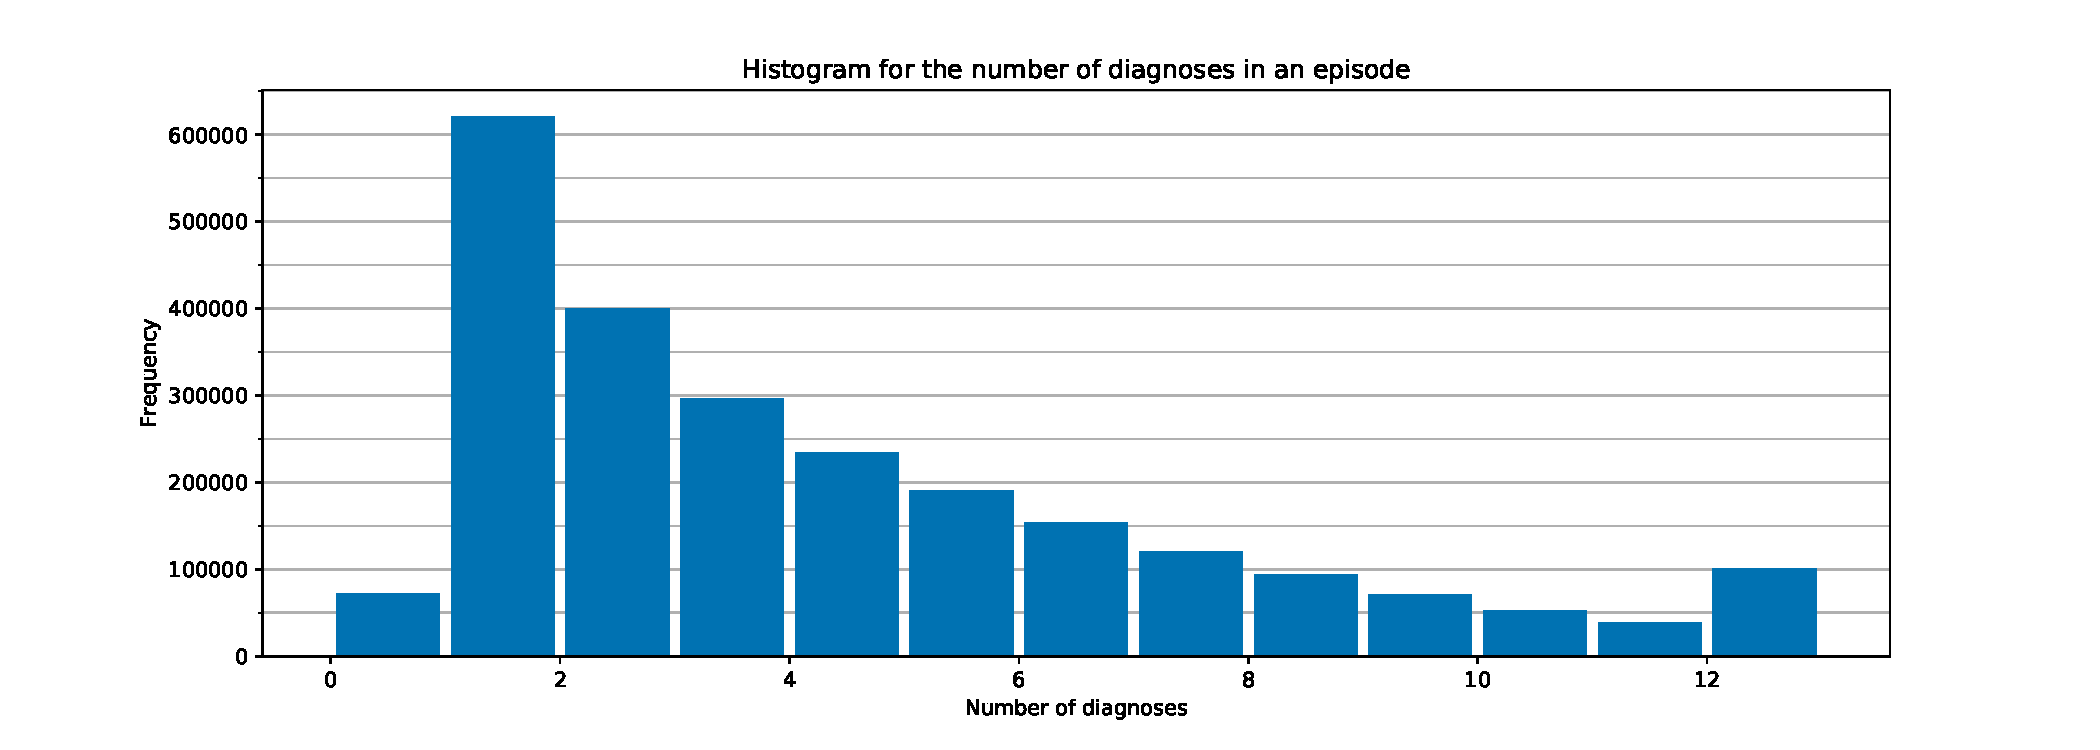
\includegraphics[width=\linewidth]{./img/diag_no_freq_hist.pdf}
        \end{minipage}
        \begin{minipage}{\linewidth}
            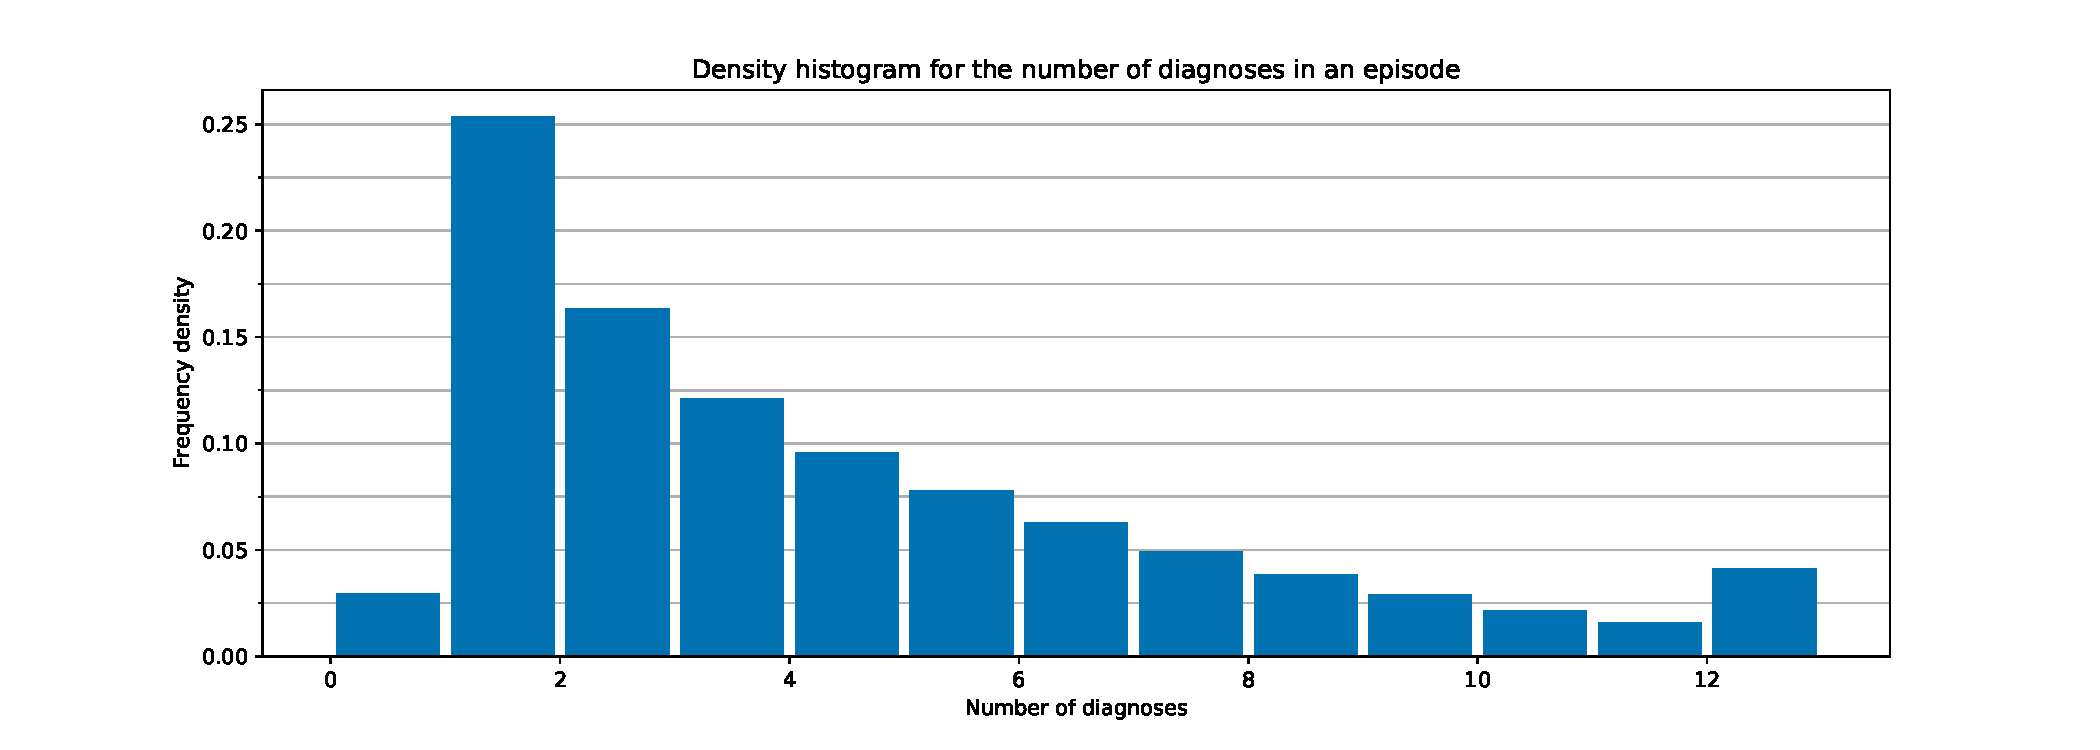
\includegraphics[width=\linewidth]{./img/diag_no_density_hist.pdf}
        \end{minipage}
    \end{figure}
\end{frame}

\begin{frame}
    \frametitle{Number of procedures}

    \begin{figure}
        \begin{minipage}{\linewidth}
            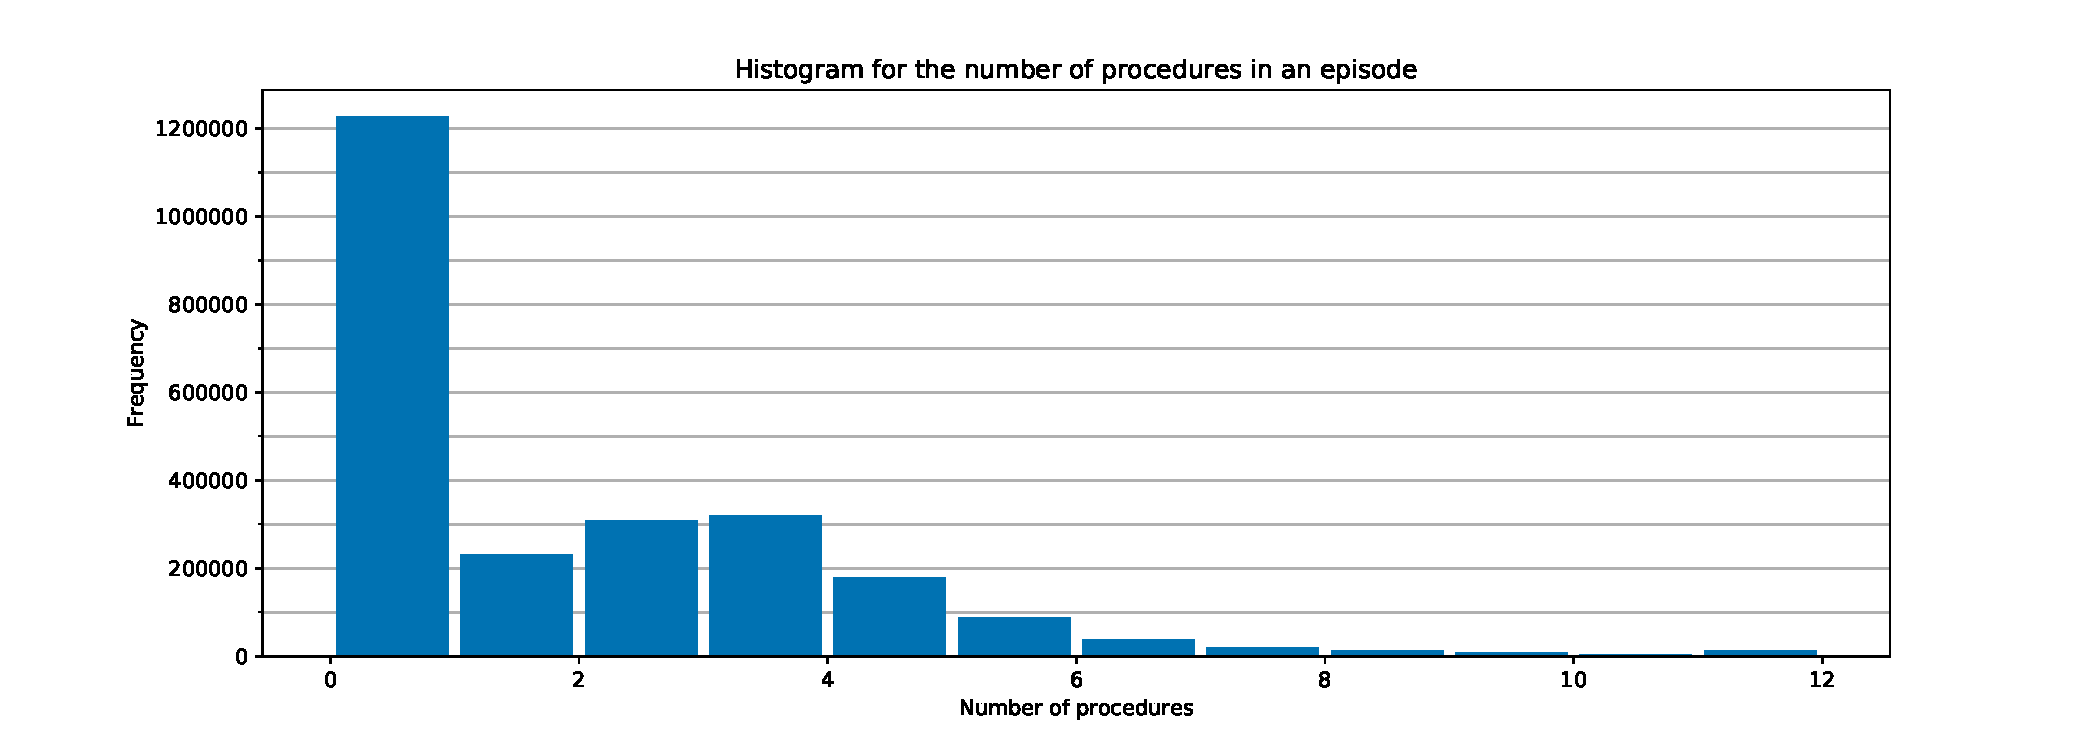
\includegraphics[width=\linewidth]{./img/proc_no_freq_hist.pdf}
        \end{minipage}
        \begin{minipage}{\linewidth}
            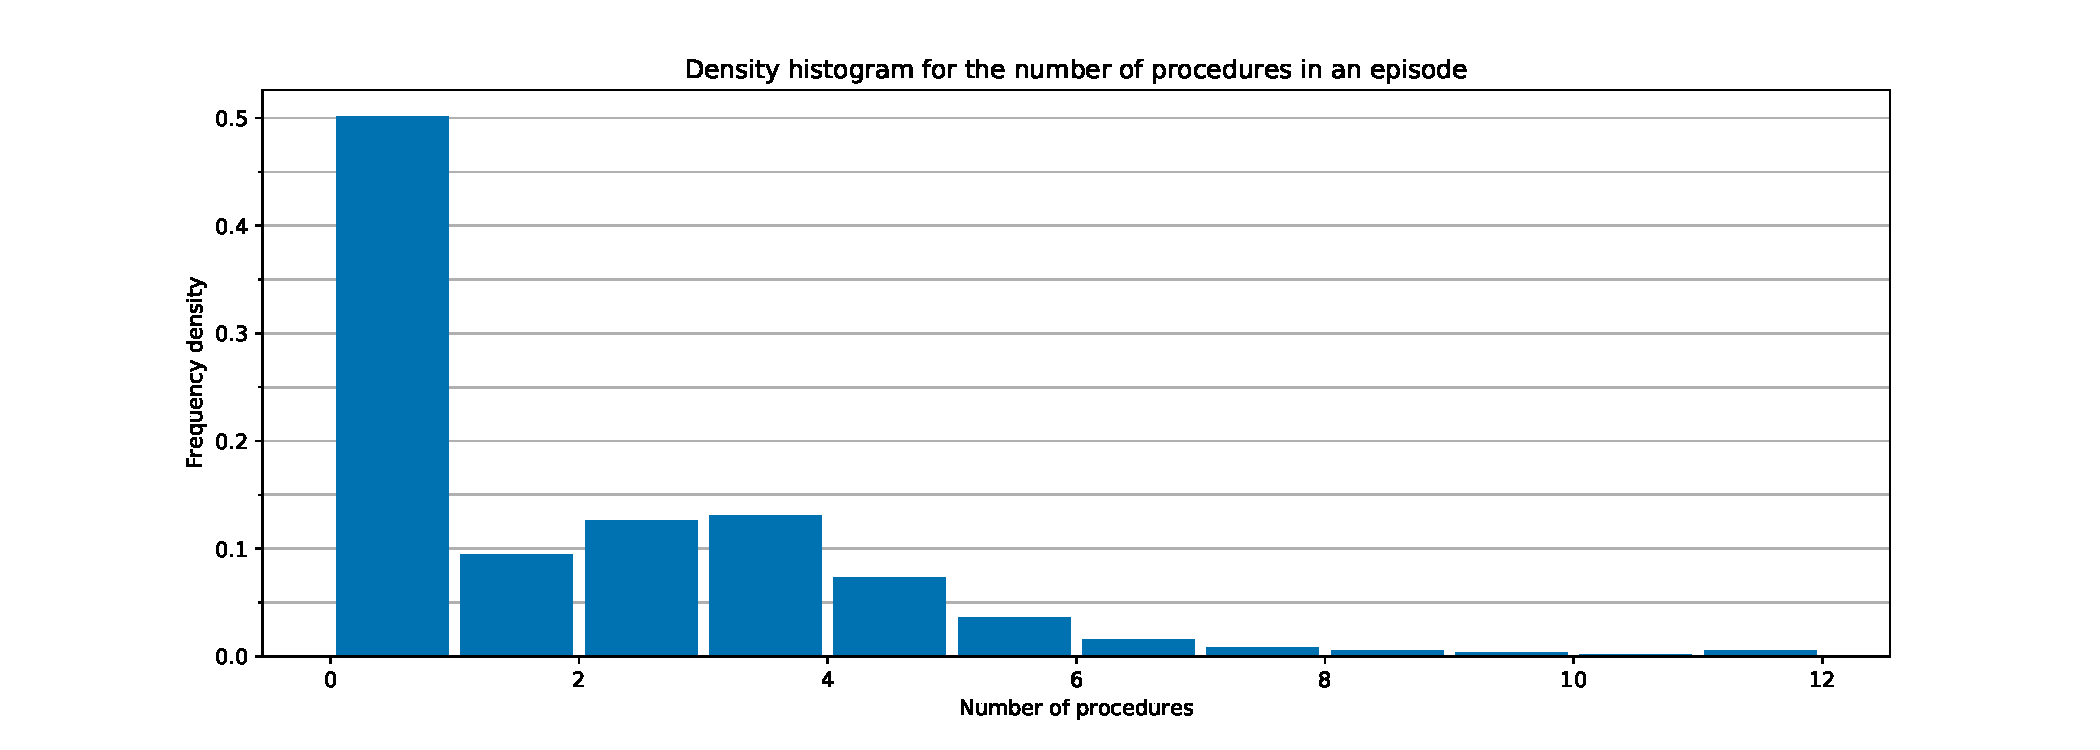
\includegraphics[width=\linewidth]{./img/proc_no_density_hist.pdf}
        \end{minipage}
    \end{figure}
\end{frame}

\begin{frame}
    \frametitle{Demographic analysis}

    As it stands, demographic information is not well-recorded in the data.

    \vspace{10pt}
    \begin{itemize}
        \pause%
        \item Gender is strictly binary and not recorded for all patients or
            episodes
        \pause%
        \item Limited geographic information is encoded in the GP practice code
            of the patient
    \end{itemize}
\end{frame}

\begin{frame}
    \frametitle{Demographic analysis}

    \begin{figure}
        \begin{minipage}{\linewidth}
            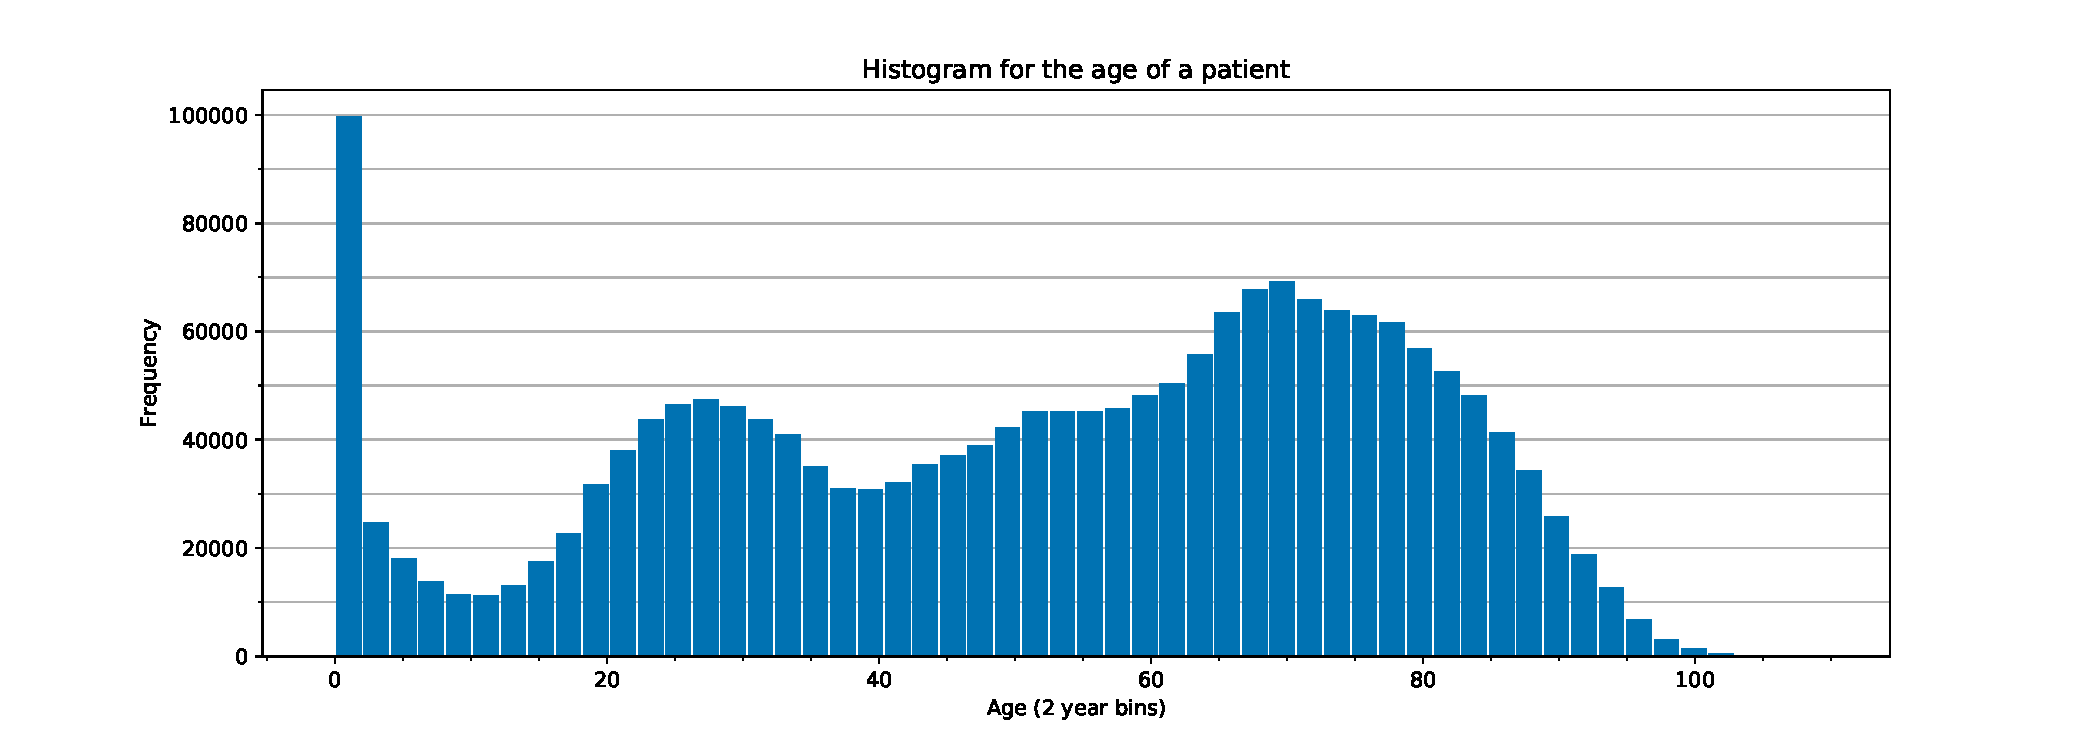
\includegraphics[width=\linewidth]{./img/age_freq_hist.pdf}
        \end{minipage}
        \begin{minipage}{\linewidth}
            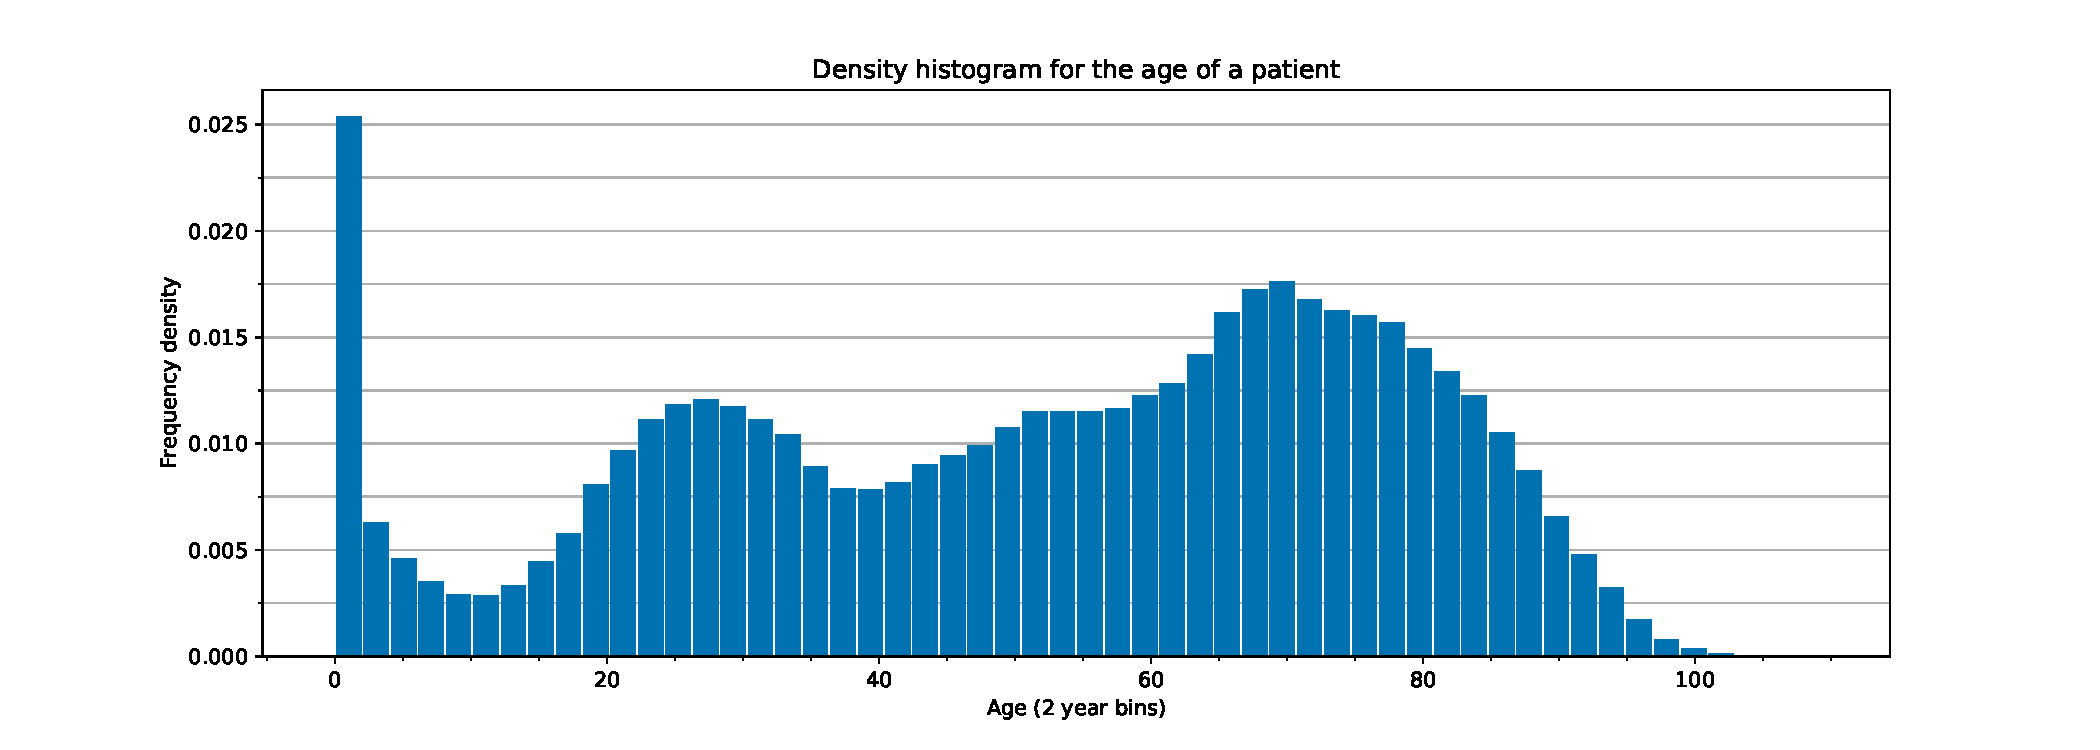
\includegraphics[width=\linewidth]{./img/age_density_hist.pdf}
        \end{minipage}
    \end{figure}
\end{frame}

\begin{frame}
    \frametitle{Correlation}

    \vspace{-15pt}
    \begin{figure}
        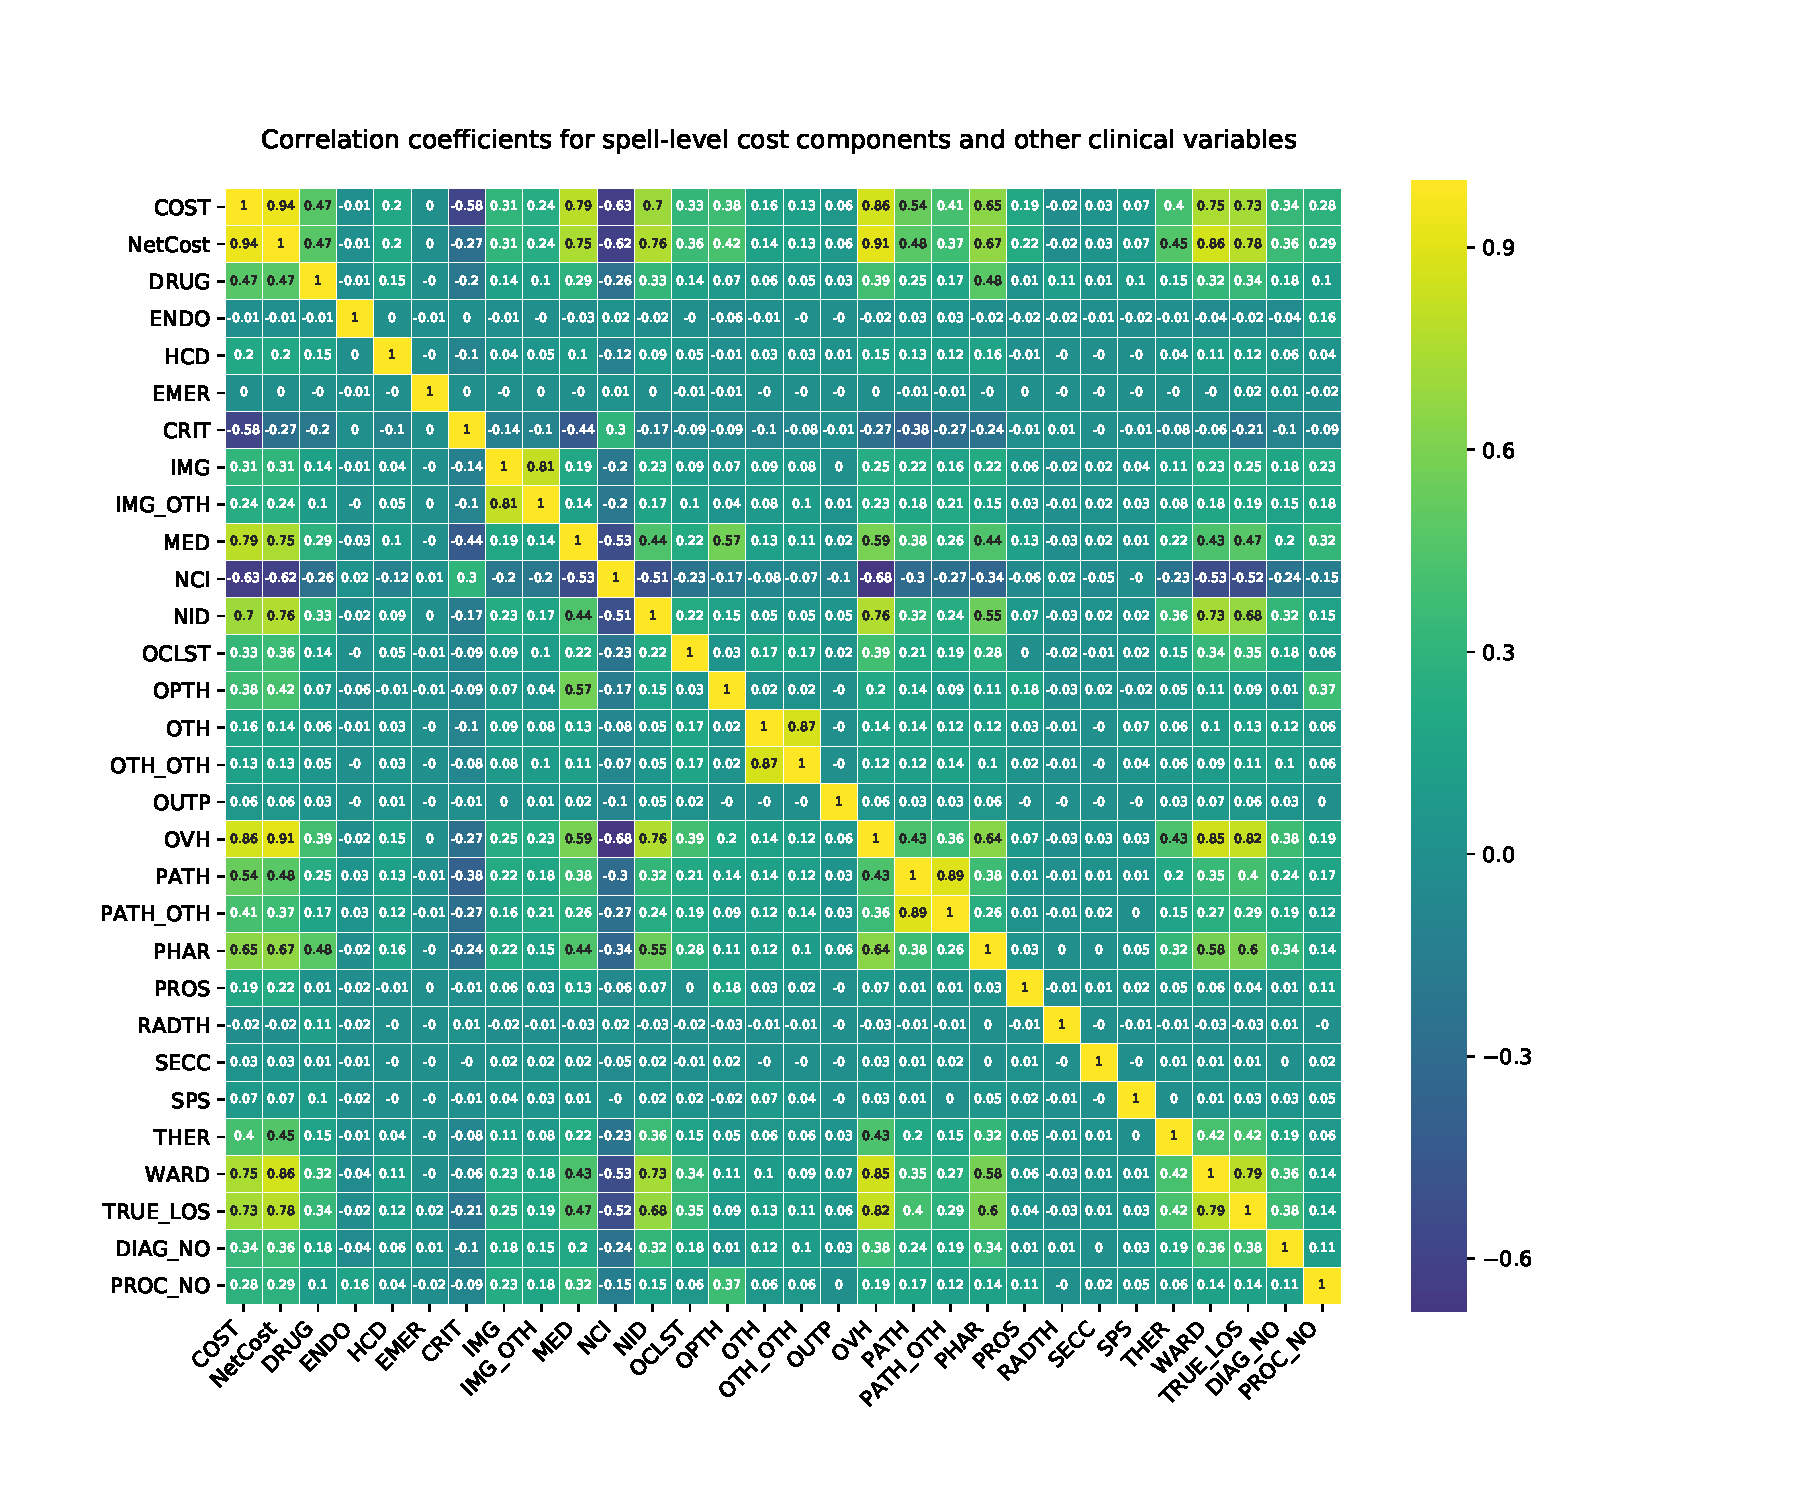
\includegraphics[width=\linewidth]{./img/corr_heatmap.pdf}
    \end{figure}
\end{frame}


\subsection{Measuring variation}

\begin{frame}
    \frametitle{Measuring variation}

    Variance is not scale invariant and did lead to misconceptions.

    \pause%
    \vspace{10pt}
    \begin{definition}
        Let \(\mu, \sigma^2\) denote the population mean and population variance
        of some population respectively. Then we define the
        \emph{coefficient~of~variation}, denoted by \(C_v\), to be:
        \[
            C_v = \frac{\sigma}{\mu}
        \]
    \end{definition}

    \pause%
    The coefficient of variation is scale invariant, and allows us to see the
    relative variation in each of our cost components.
\end{frame}

\begin{frame}
    \frametitle{Measuring variation}

    \begin{figure}
        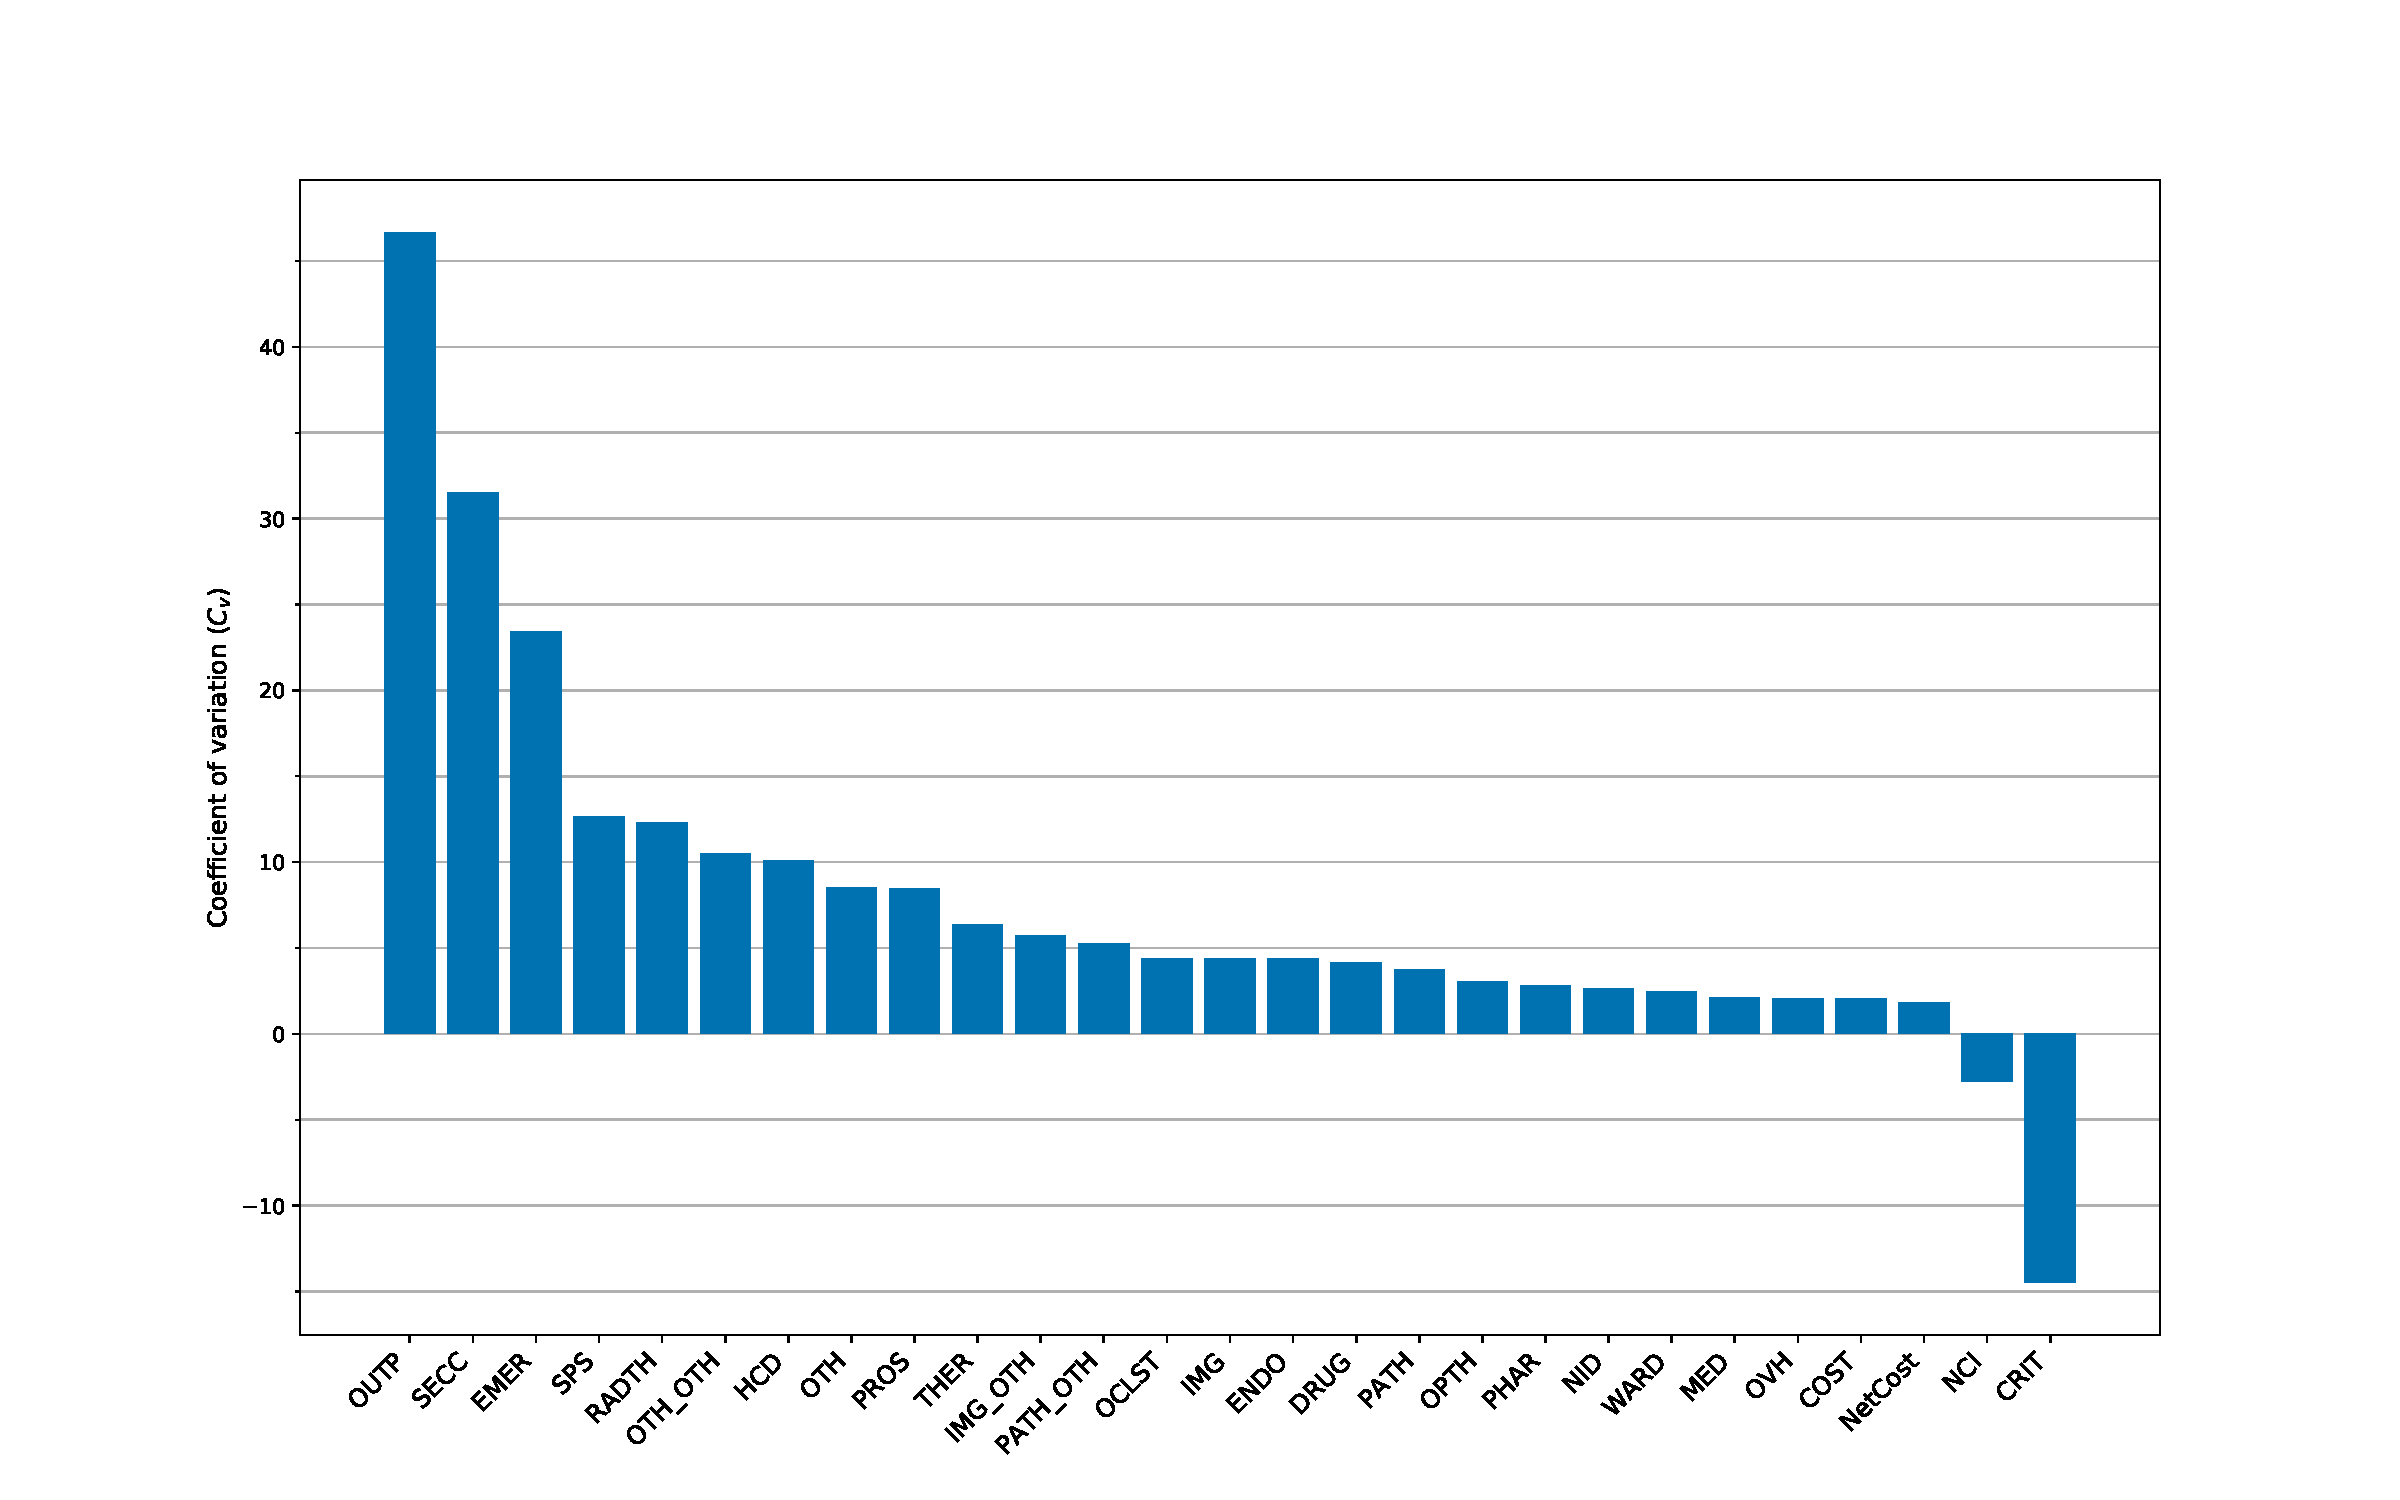
\includegraphics[width=\linewidth]{./img/coeff_variation.pdf}
    \end{figure}
\end{frame}

\begin{frame}
    \frametitle{Are these actually important?}

    Despite the relative variation of our cost components being whatever value,
    does it matter to the actual cost?

    \vspace{10pt}
    Let us investigate their contribution to the final cost.
\end{frame}

\begin{frame}
    \frametitle{Cost component contribution}

    \begin{figure}
        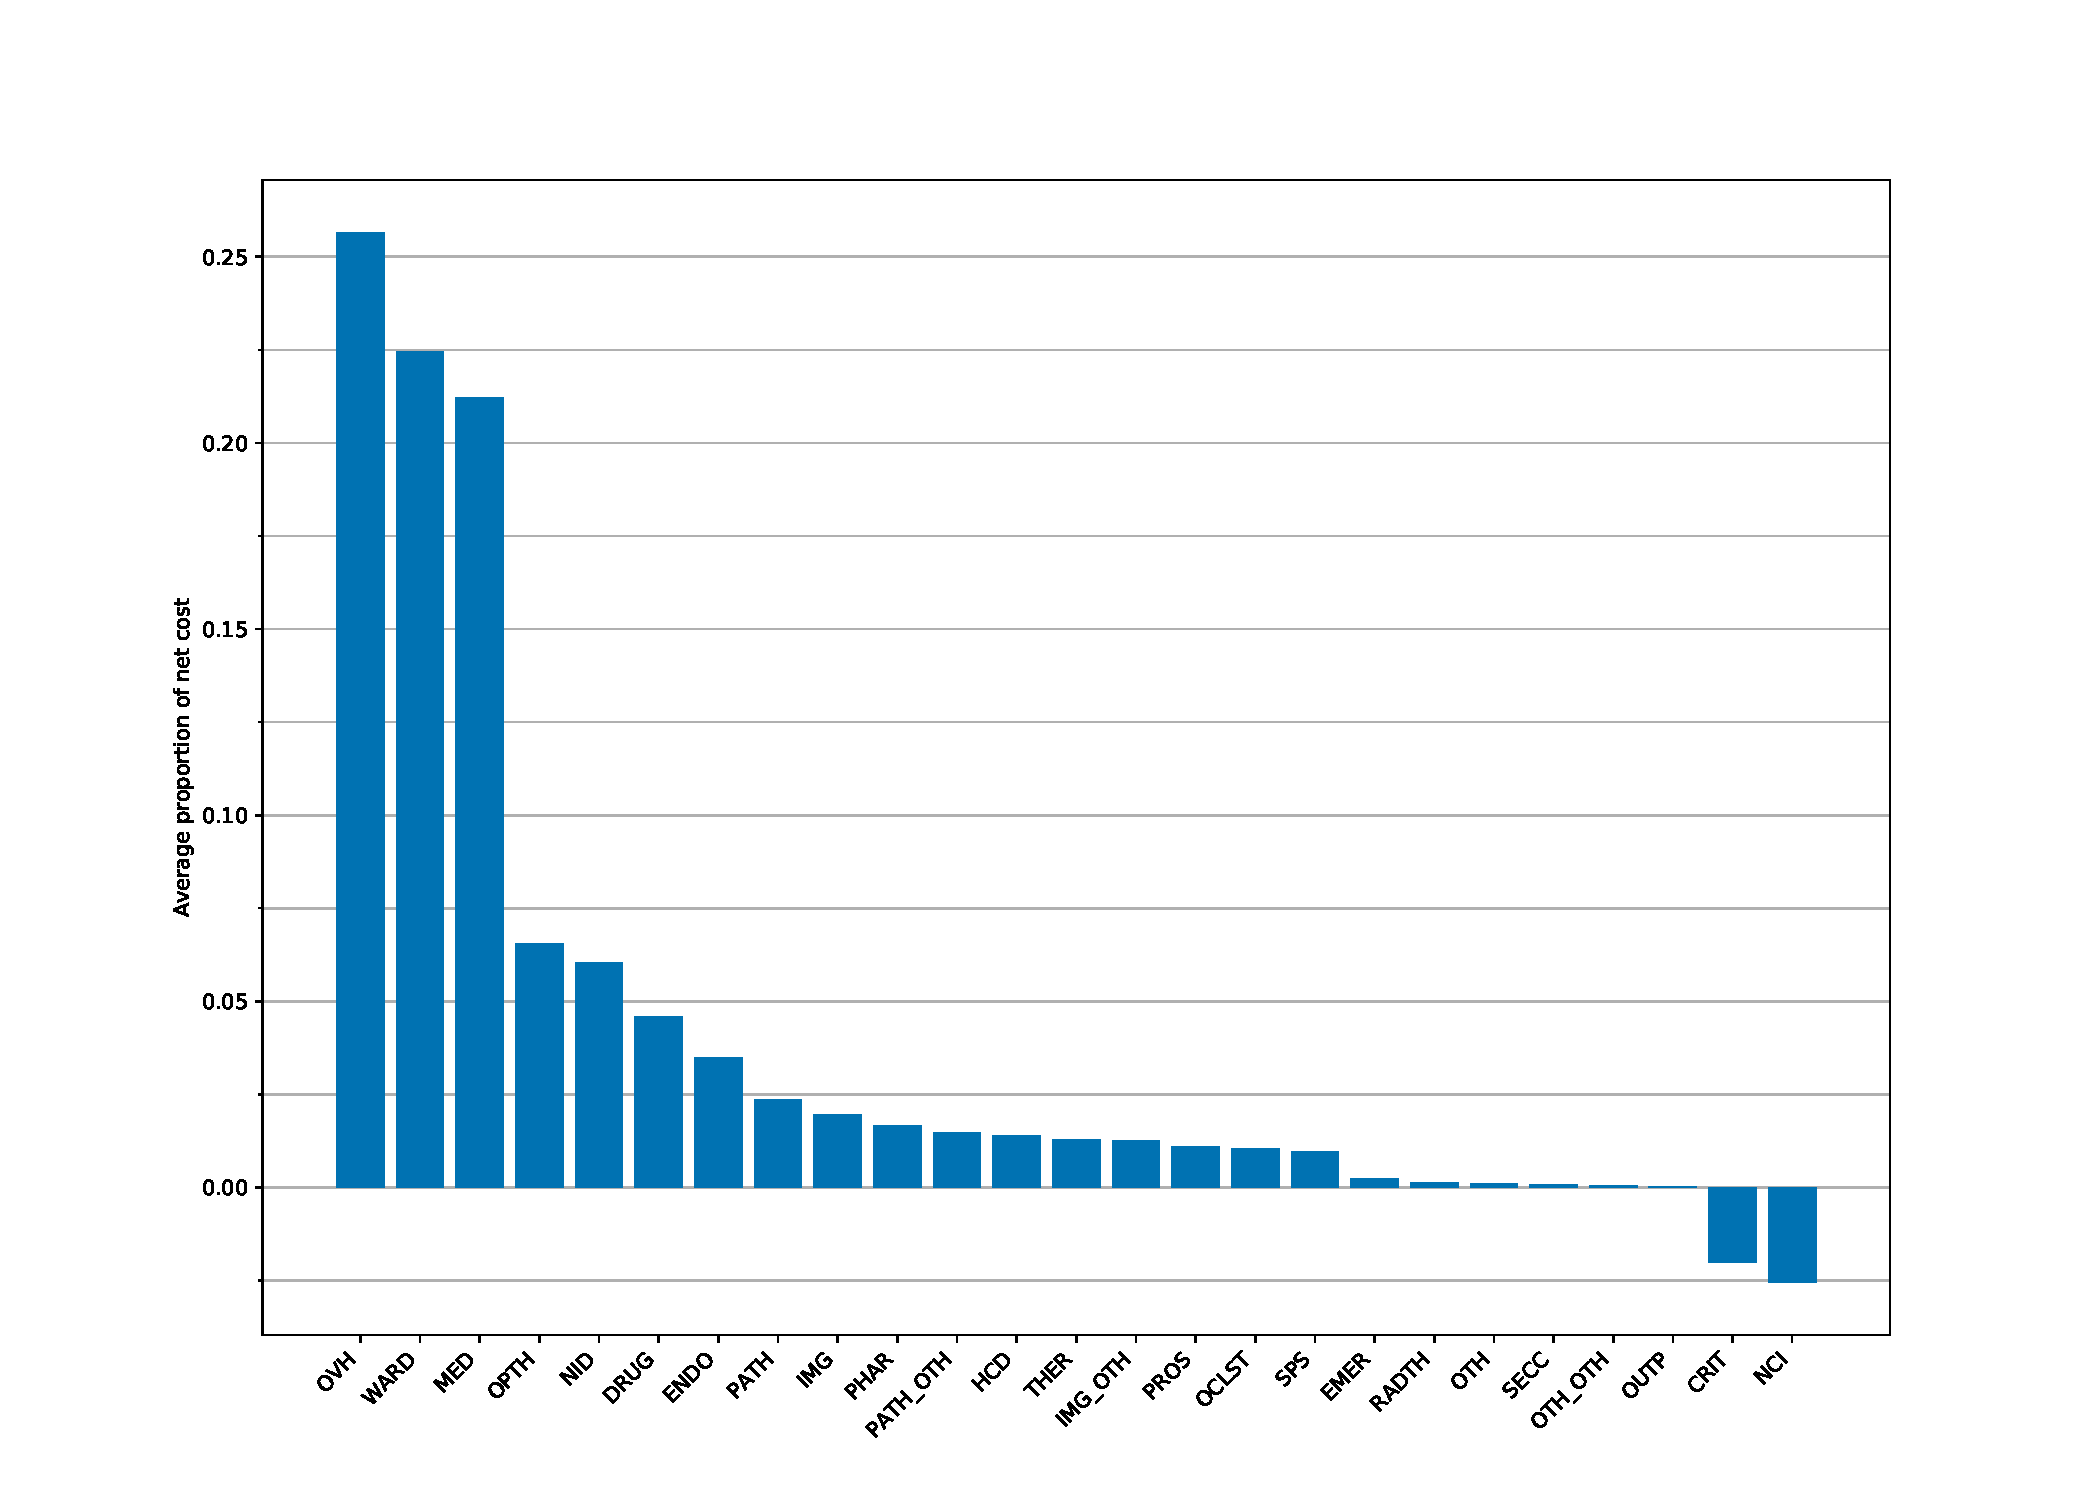
\includegraphics[width=\linewidth]{./img/cost_contribution.pdf}
    \end{figure}
\end{frame}


\section{Slice analysis}

\subsection{General methodology}

\begin{frame}
    \frametitle{General methods for slice analysis}

    Given some slice of the data, we want to:
    \begin{itemize}
        \item Examine cost variations and general surface-level statistics
        \item Determine components and variable relationships of interest
        \item Consider the relative `cost' of the patients in this slice
        \item Contrast this against its complement and the general dataset
    \end{itemize}
\end{frame}

\subsection{Diabetic patient analysis}

\begin{frame}
    \frametitle{Diabetic patient analysis}

    This is a known area of interest to the health board.

    \vspace{10pt}
    Diabetic patients make up 10.8\% of all the episodes in the dataset, and
    roughly 8.7\% of the unique patients in the dataset.

    \vspace{10pt}
    Here we consider patients to be `diabetic' if they have diabetes flagged as
    either a primary or secondary condition in their episode.
\end{frame}

\begin{frame}
    \frametitle{Number of spells}

    \begin{figure}
        \begin{minipage}{\linewidth}
            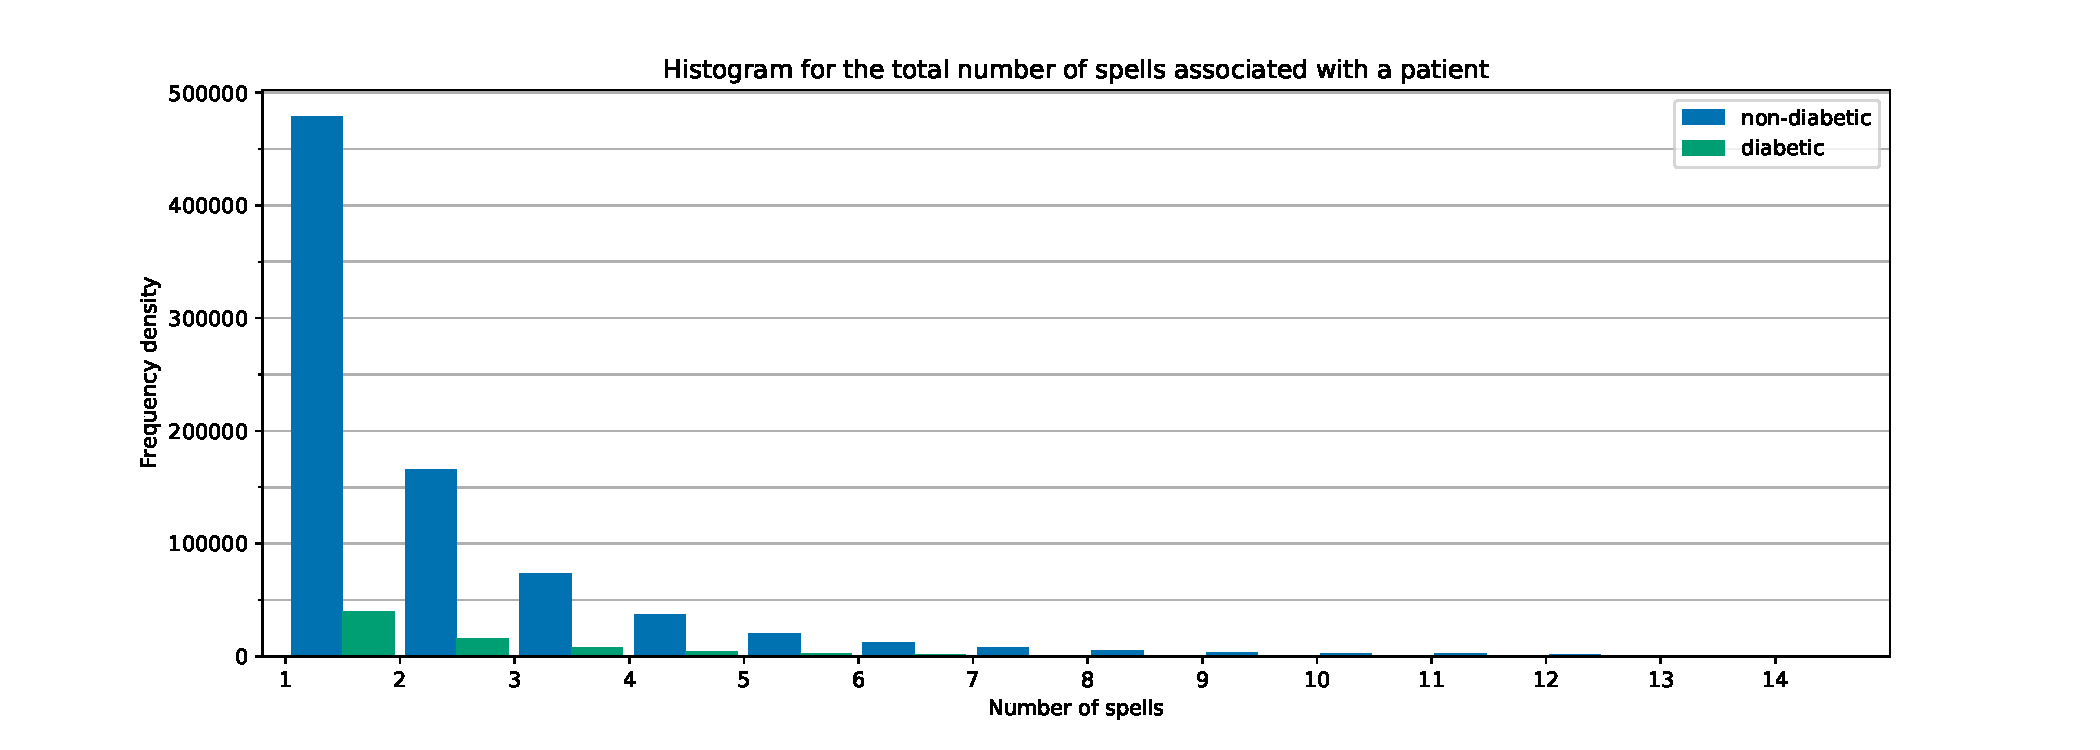
\includegraphics[width=\linewidth]
                {./img/diabetic_no_spells_freq_hist.pdf}
        \end{minipage}
        \begin{minipage}{\linewidth}
            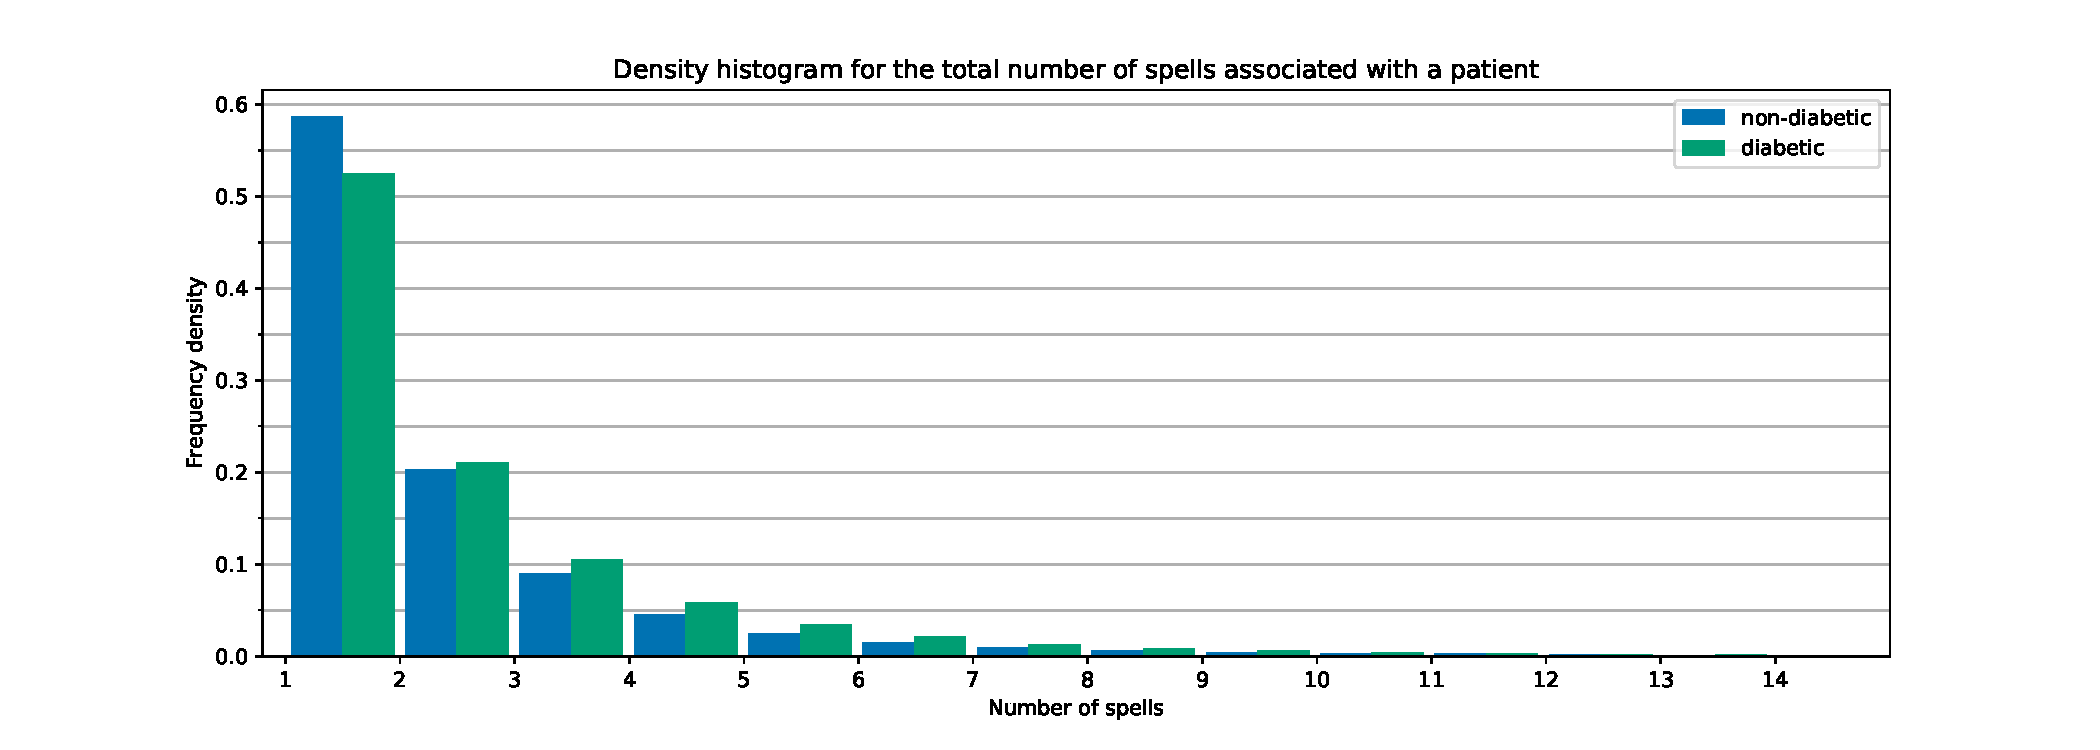
\includegraphics[width=\linewidth]
                {./img/diabetic_no_spells_density_hist.pdf}
        \end{minipage}
    \end{figure}
\end{frame}

\begin{frame}
    \frametitle{Length of stay}

    \begin{figure}
        \begin{minipage}{\linewidth}
            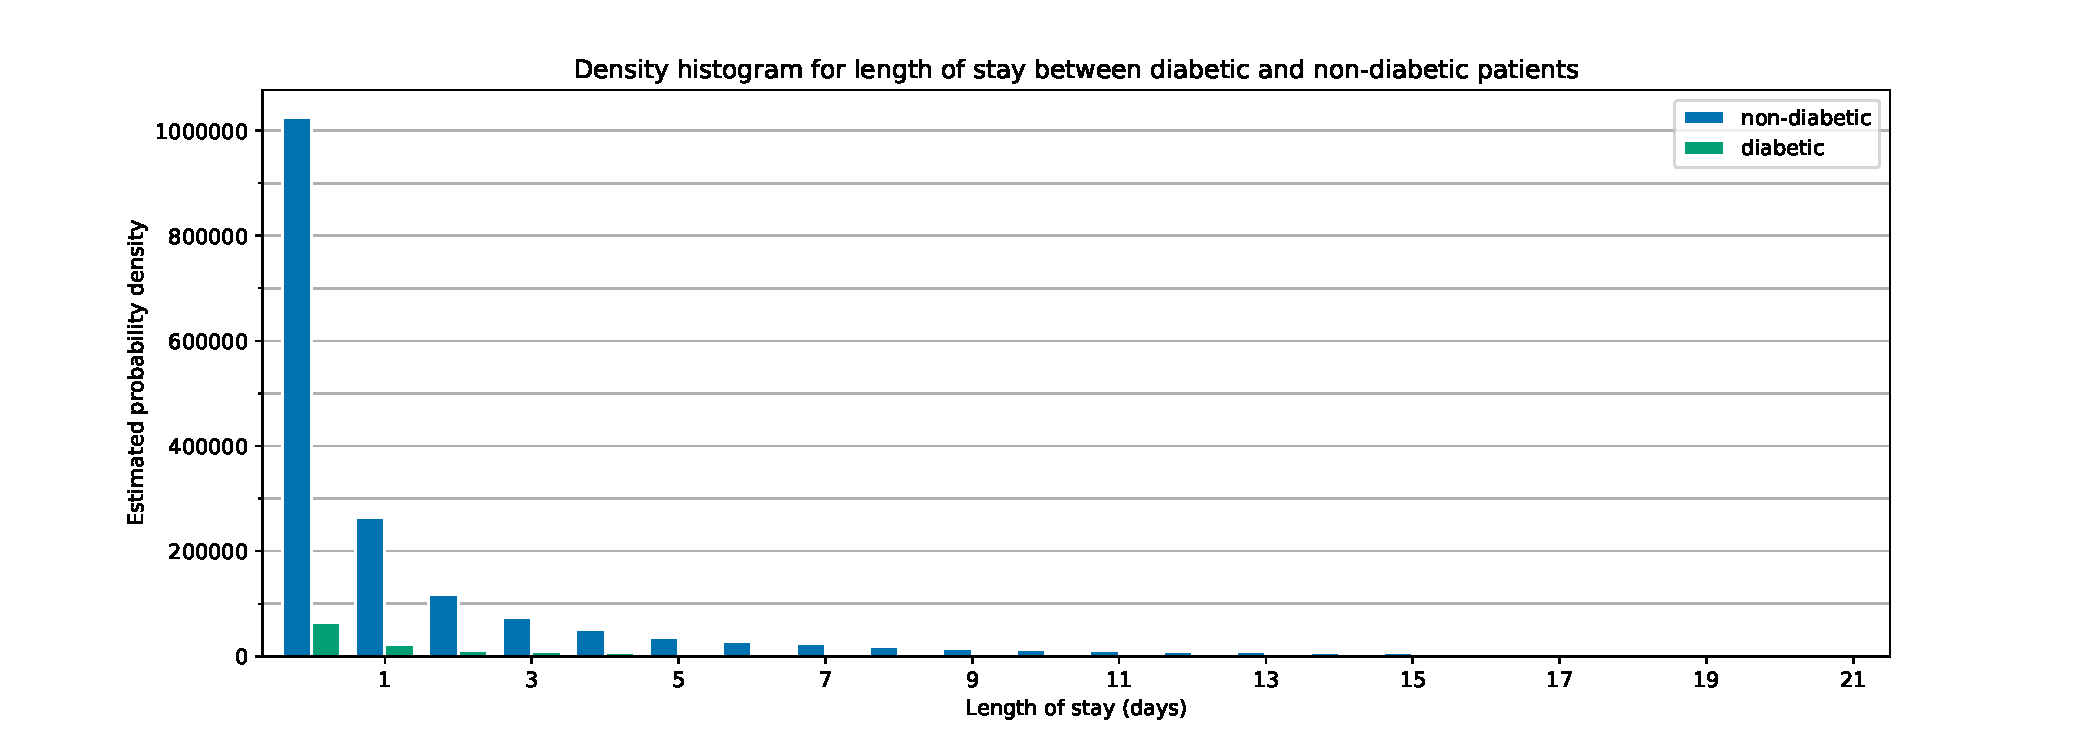
\includegraphics[width=\linewidth]{./img/diabetic_LOS_freq_hist.pdf}
        \end{minipage}
        \begin{minipage}{\linewidth}
            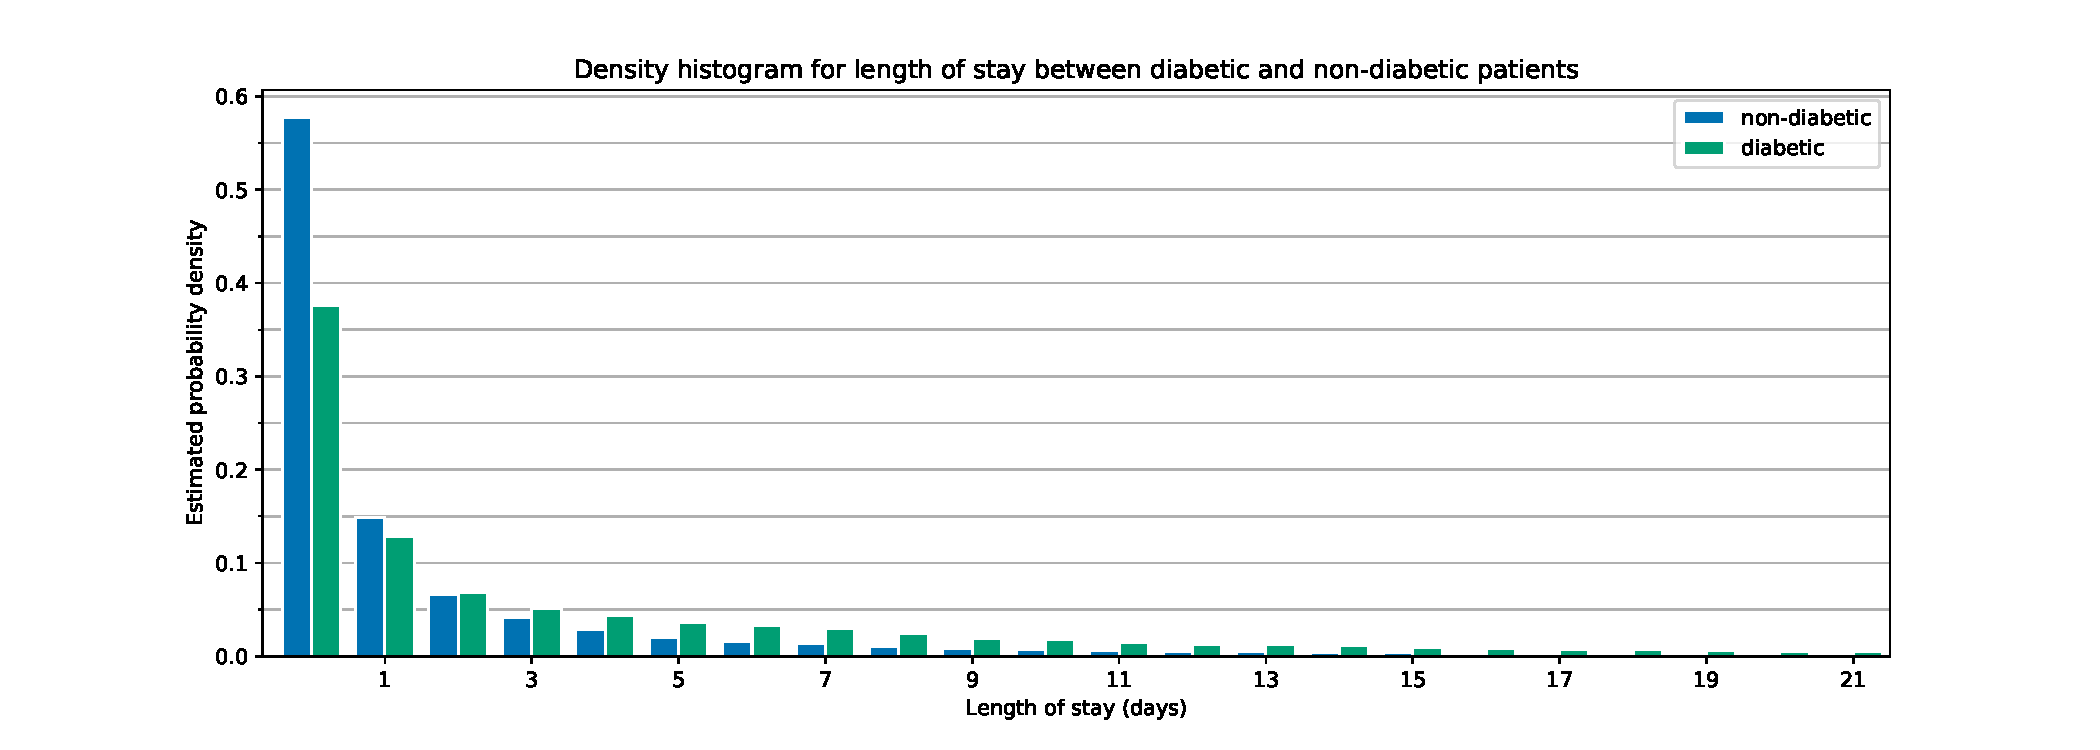
\includegraphics[width=\linewidth]
                {./img/diabetic_LOS_density_hist.pdf}
        \end{minipage}
    \end{figure}
\end{frame}

\begin{frame}
    \frametitle{Net cost}

    \begin{figure}
        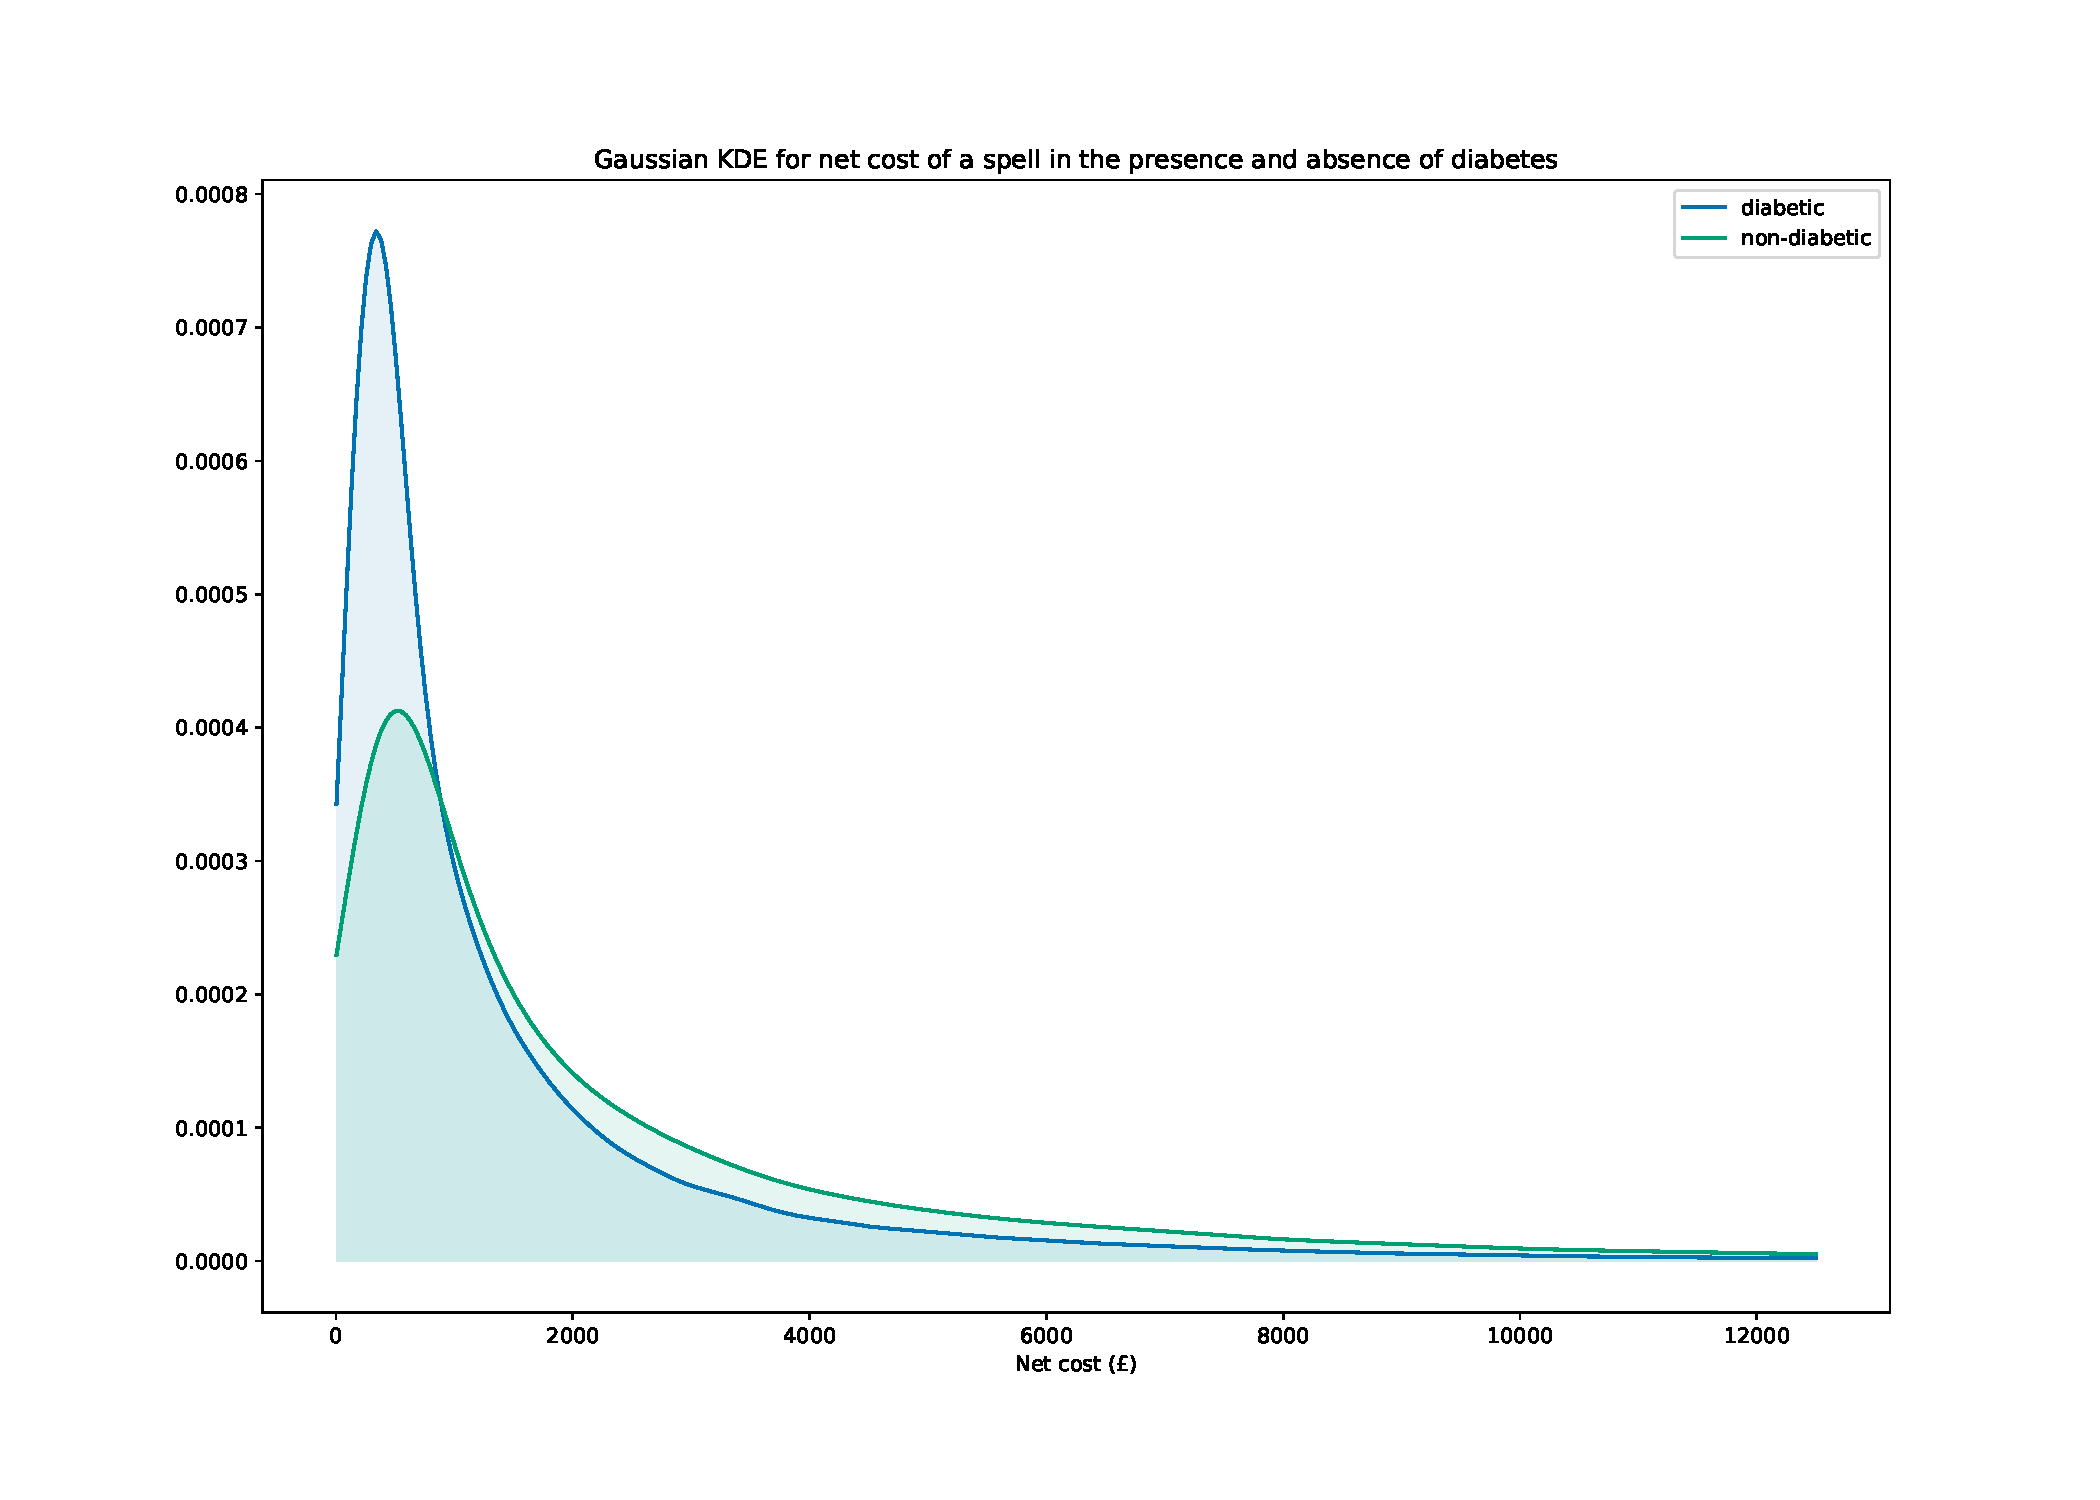
\includegraphics[width=\linewidth]{./img/diabetic_netcost_kde.pdf}
    \end{figure}
\end{frame}

\begin{frame}
    \frametitle{Number of diagnoses}
   
    \begin{figure}
        \begin{minipage}{\linewidth}
            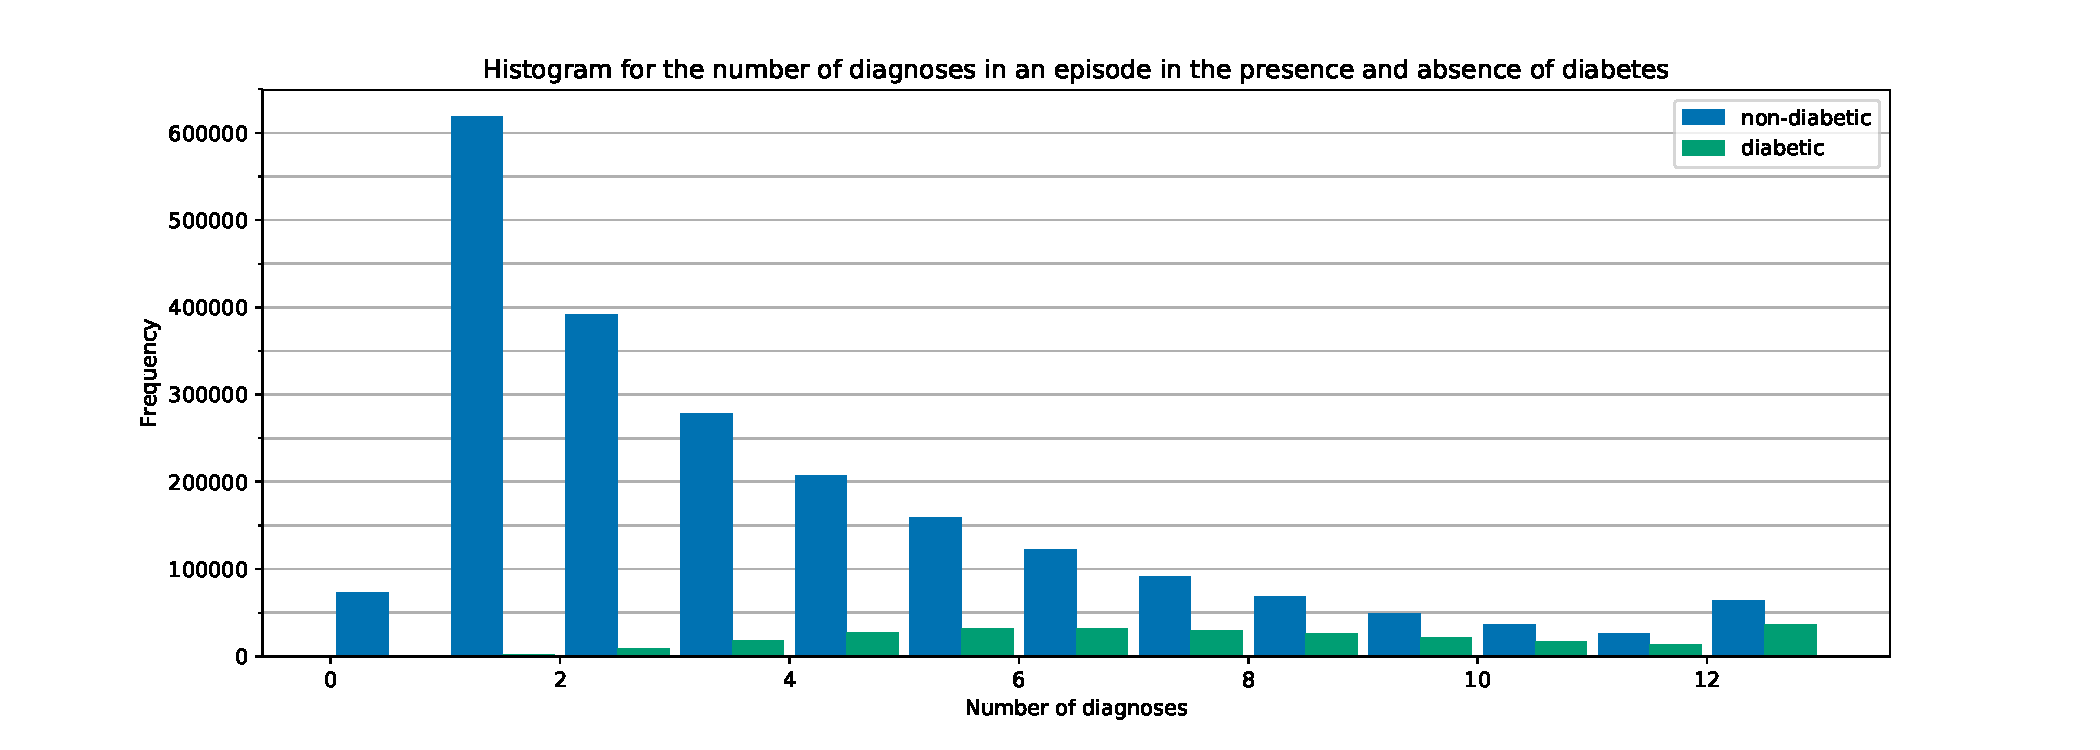
\includegraphics[width=\linewidth]
                {./img/diabetic_diag_no_freq_hist.pdf}
        \end{minipage}
        \begin{minipage}{\linewidth}
            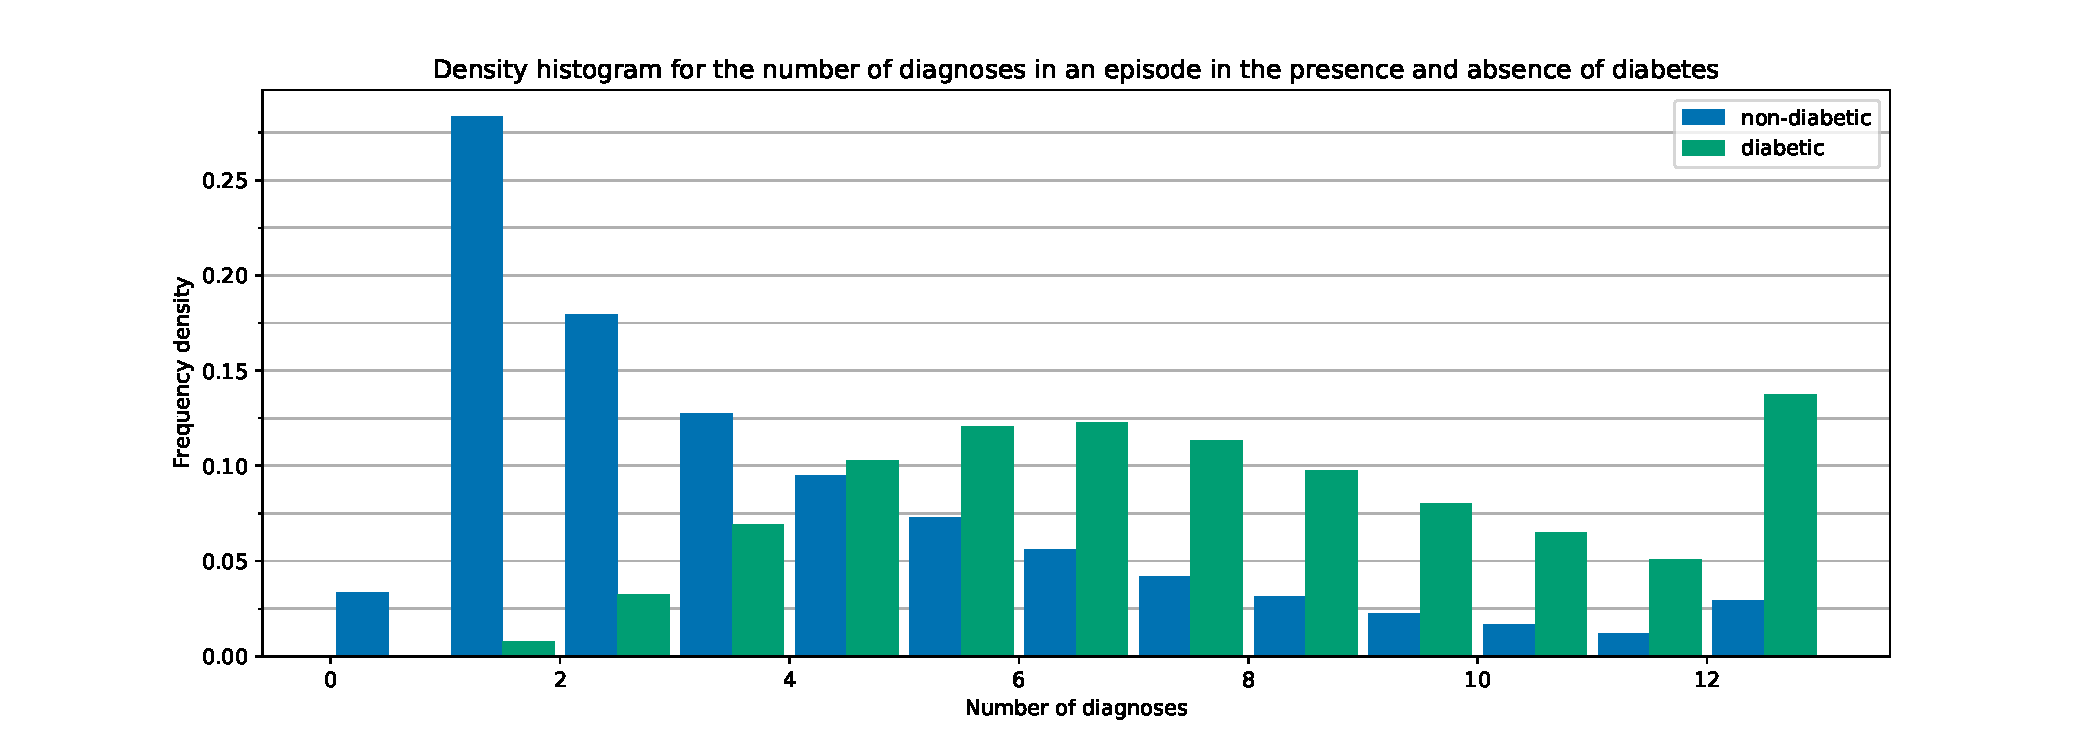
\includegraphics[width=\linewidth]
                {./img/diabetic_diag_no_density_hist.pdf}
        \end{minipage}
    \end{figure}
\end{frame}

\begin{frame}
    \frametitle{Number of procedures}

    \begin{figure}
        \begin{minipage}{\linewidth}
            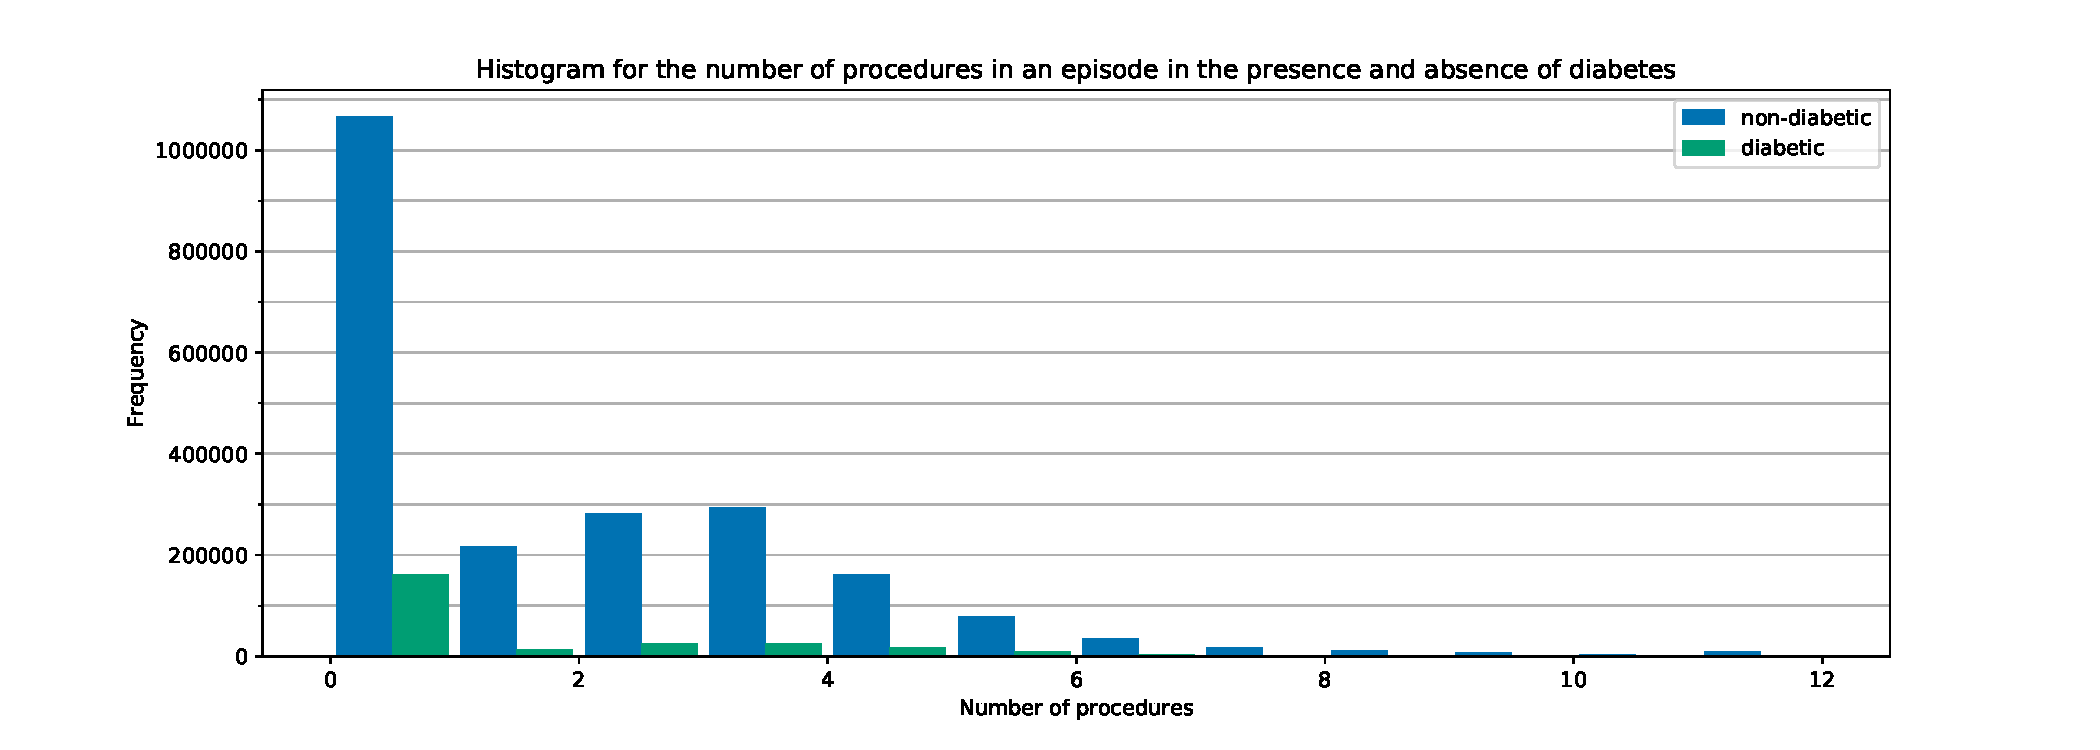
\includegraphics[width=\linewidth]
                {./img/diabetic_proc_no_freq_hist.pdf}
        \end{minipage}
        \begin{minipage}{\linewidth}
            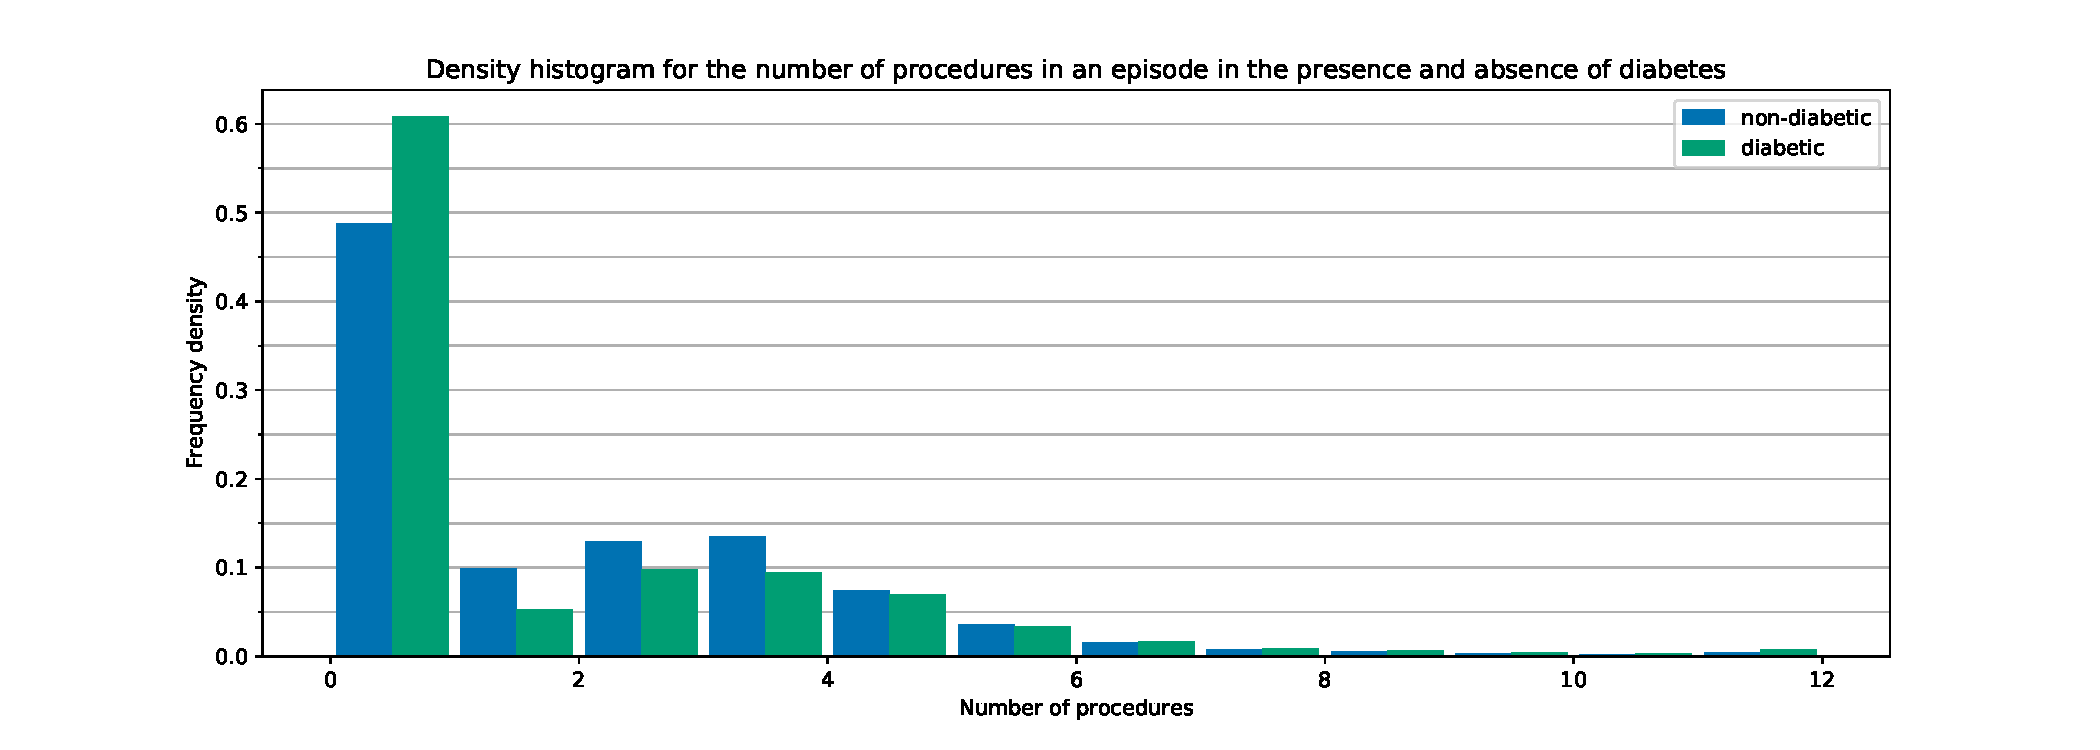
\includegraphics[width=\linewidth]
                {./img/diabetic_proc_no_density_hist.pdf}
        \end{minipage}
    \end{figure}
\end{frame}

\begin{frame}
    \frametitle{Demographic analysis}

    \begin{figure}
        \begin{minipage}{\linewidth}
            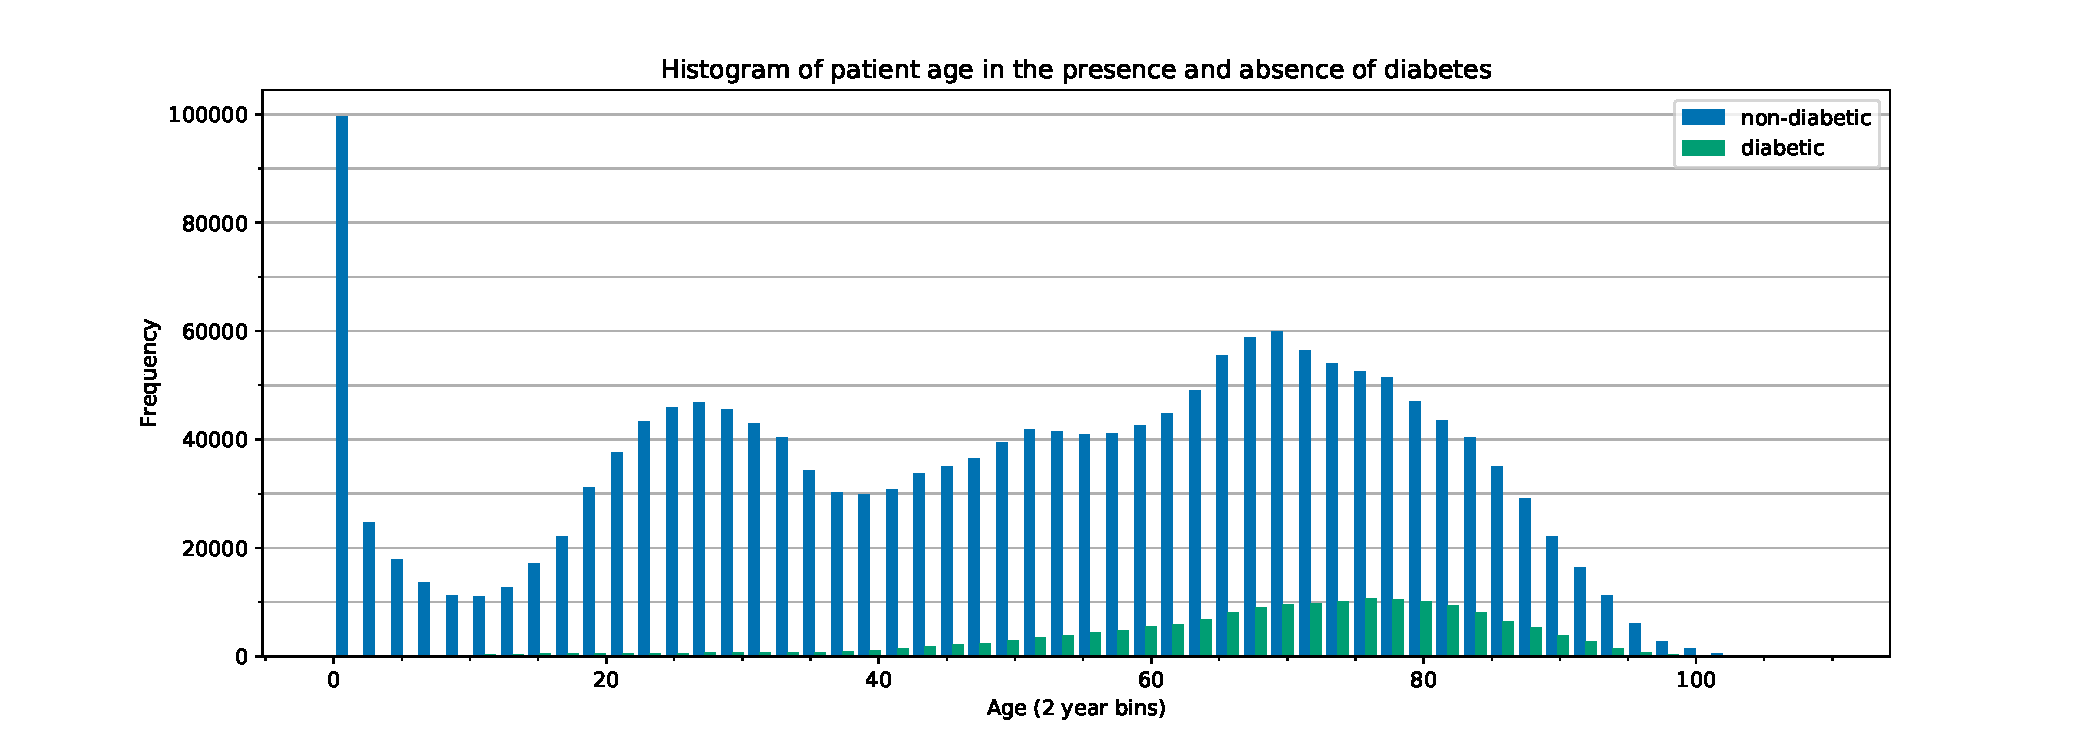
\includegraphics[width=\linewidth]{./img/diabetic_age_freq_hist.pdf}
        \end{minipage}
        \begin{minipage}{\linewidth}
            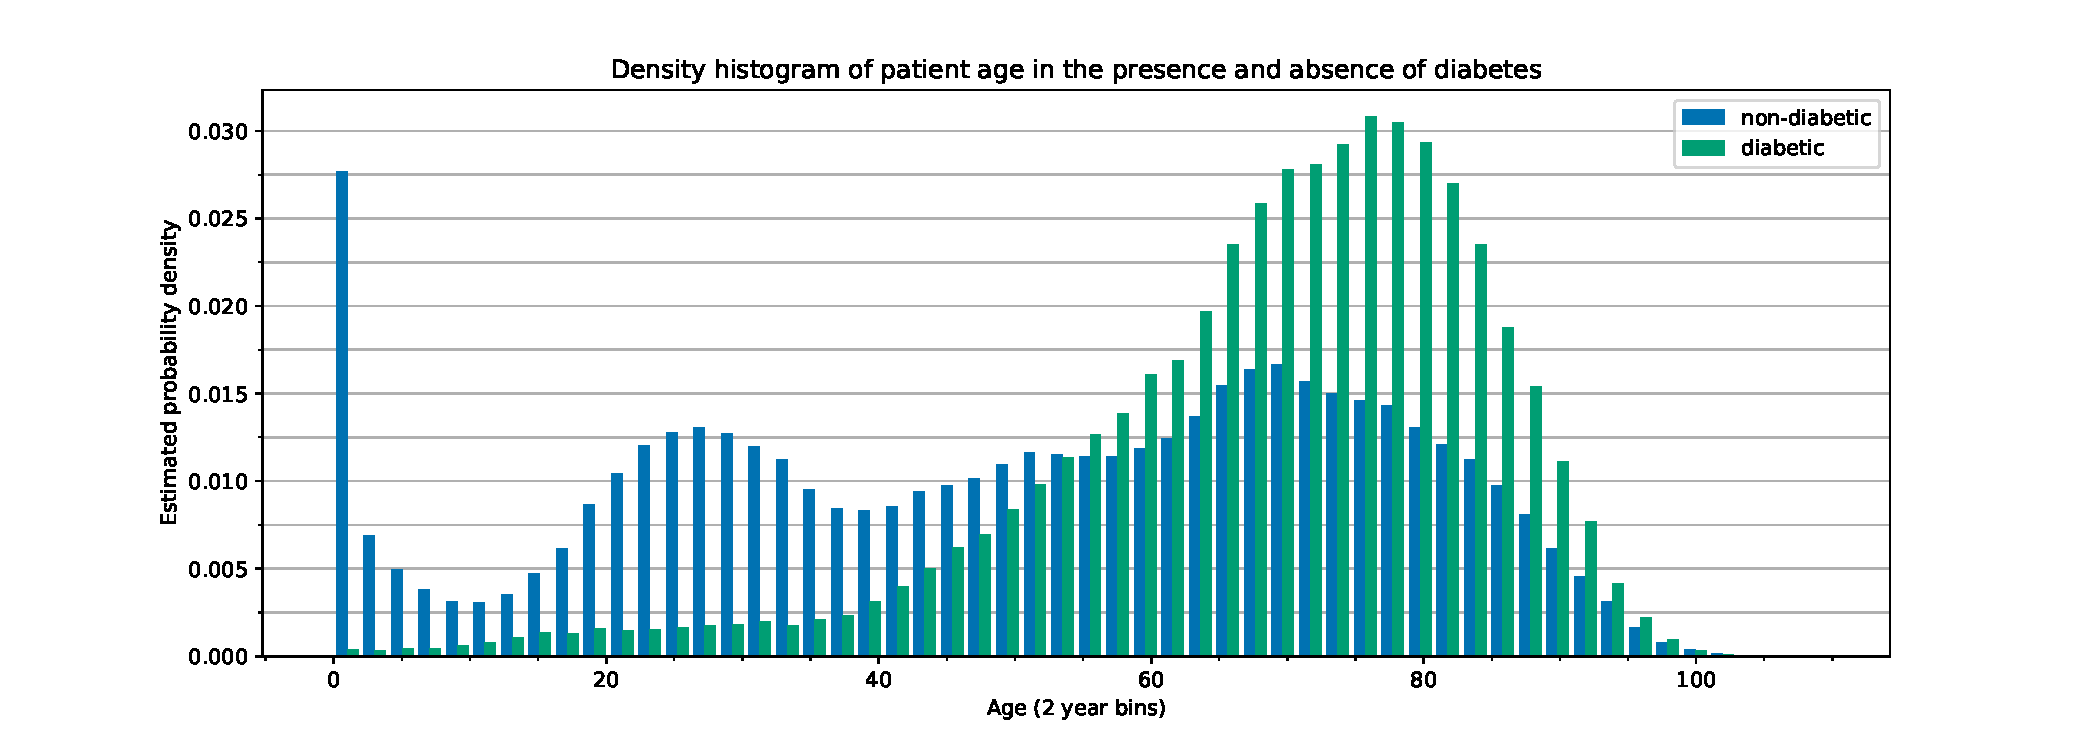
\includegraphics[width=\linewidth]
                {./img/diabetic_age_density_hist.pdf}
        \end{minipage}
    \end{figure}
\end{frame}

\begin{frame}
    \frametitle{Cost variation}

    \begin{figure}
        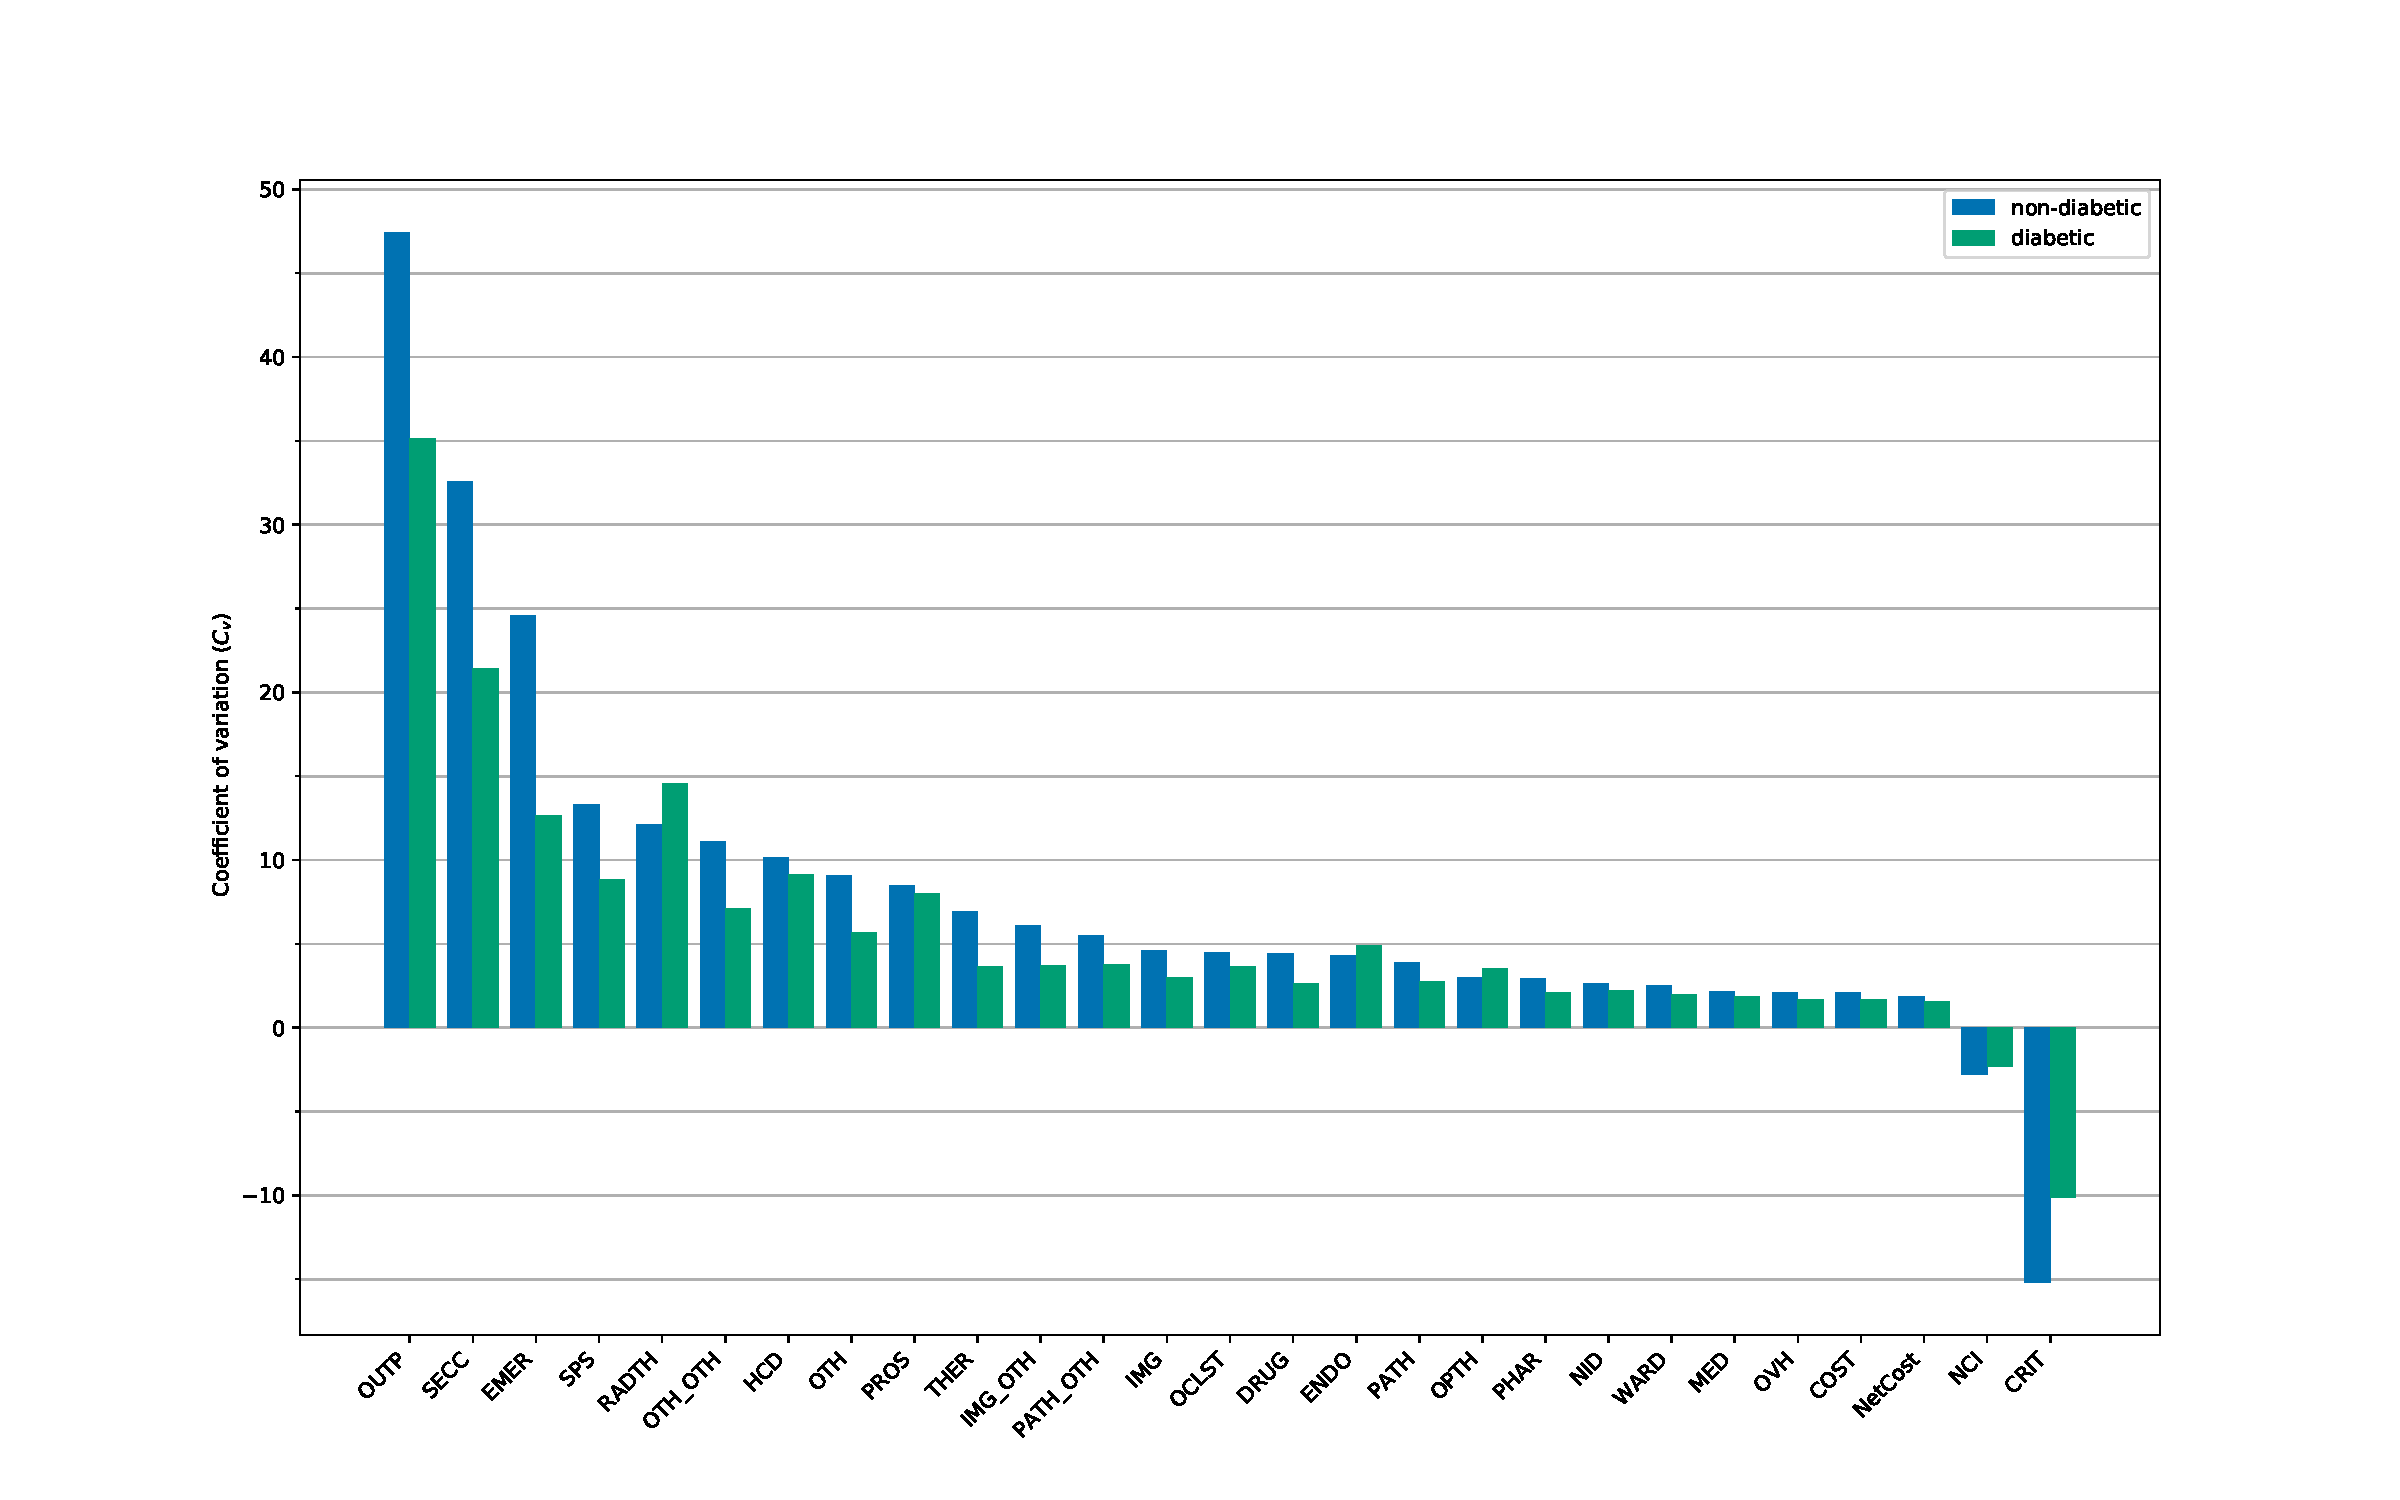
\includegraphics[width=\linewidth]{./img/diabetic_coeff_variation.pdf}
    \end{figure}
\end{frame}

\begin{frame}
    \frametitle{Cost component contribution}

    \begin{figure}
        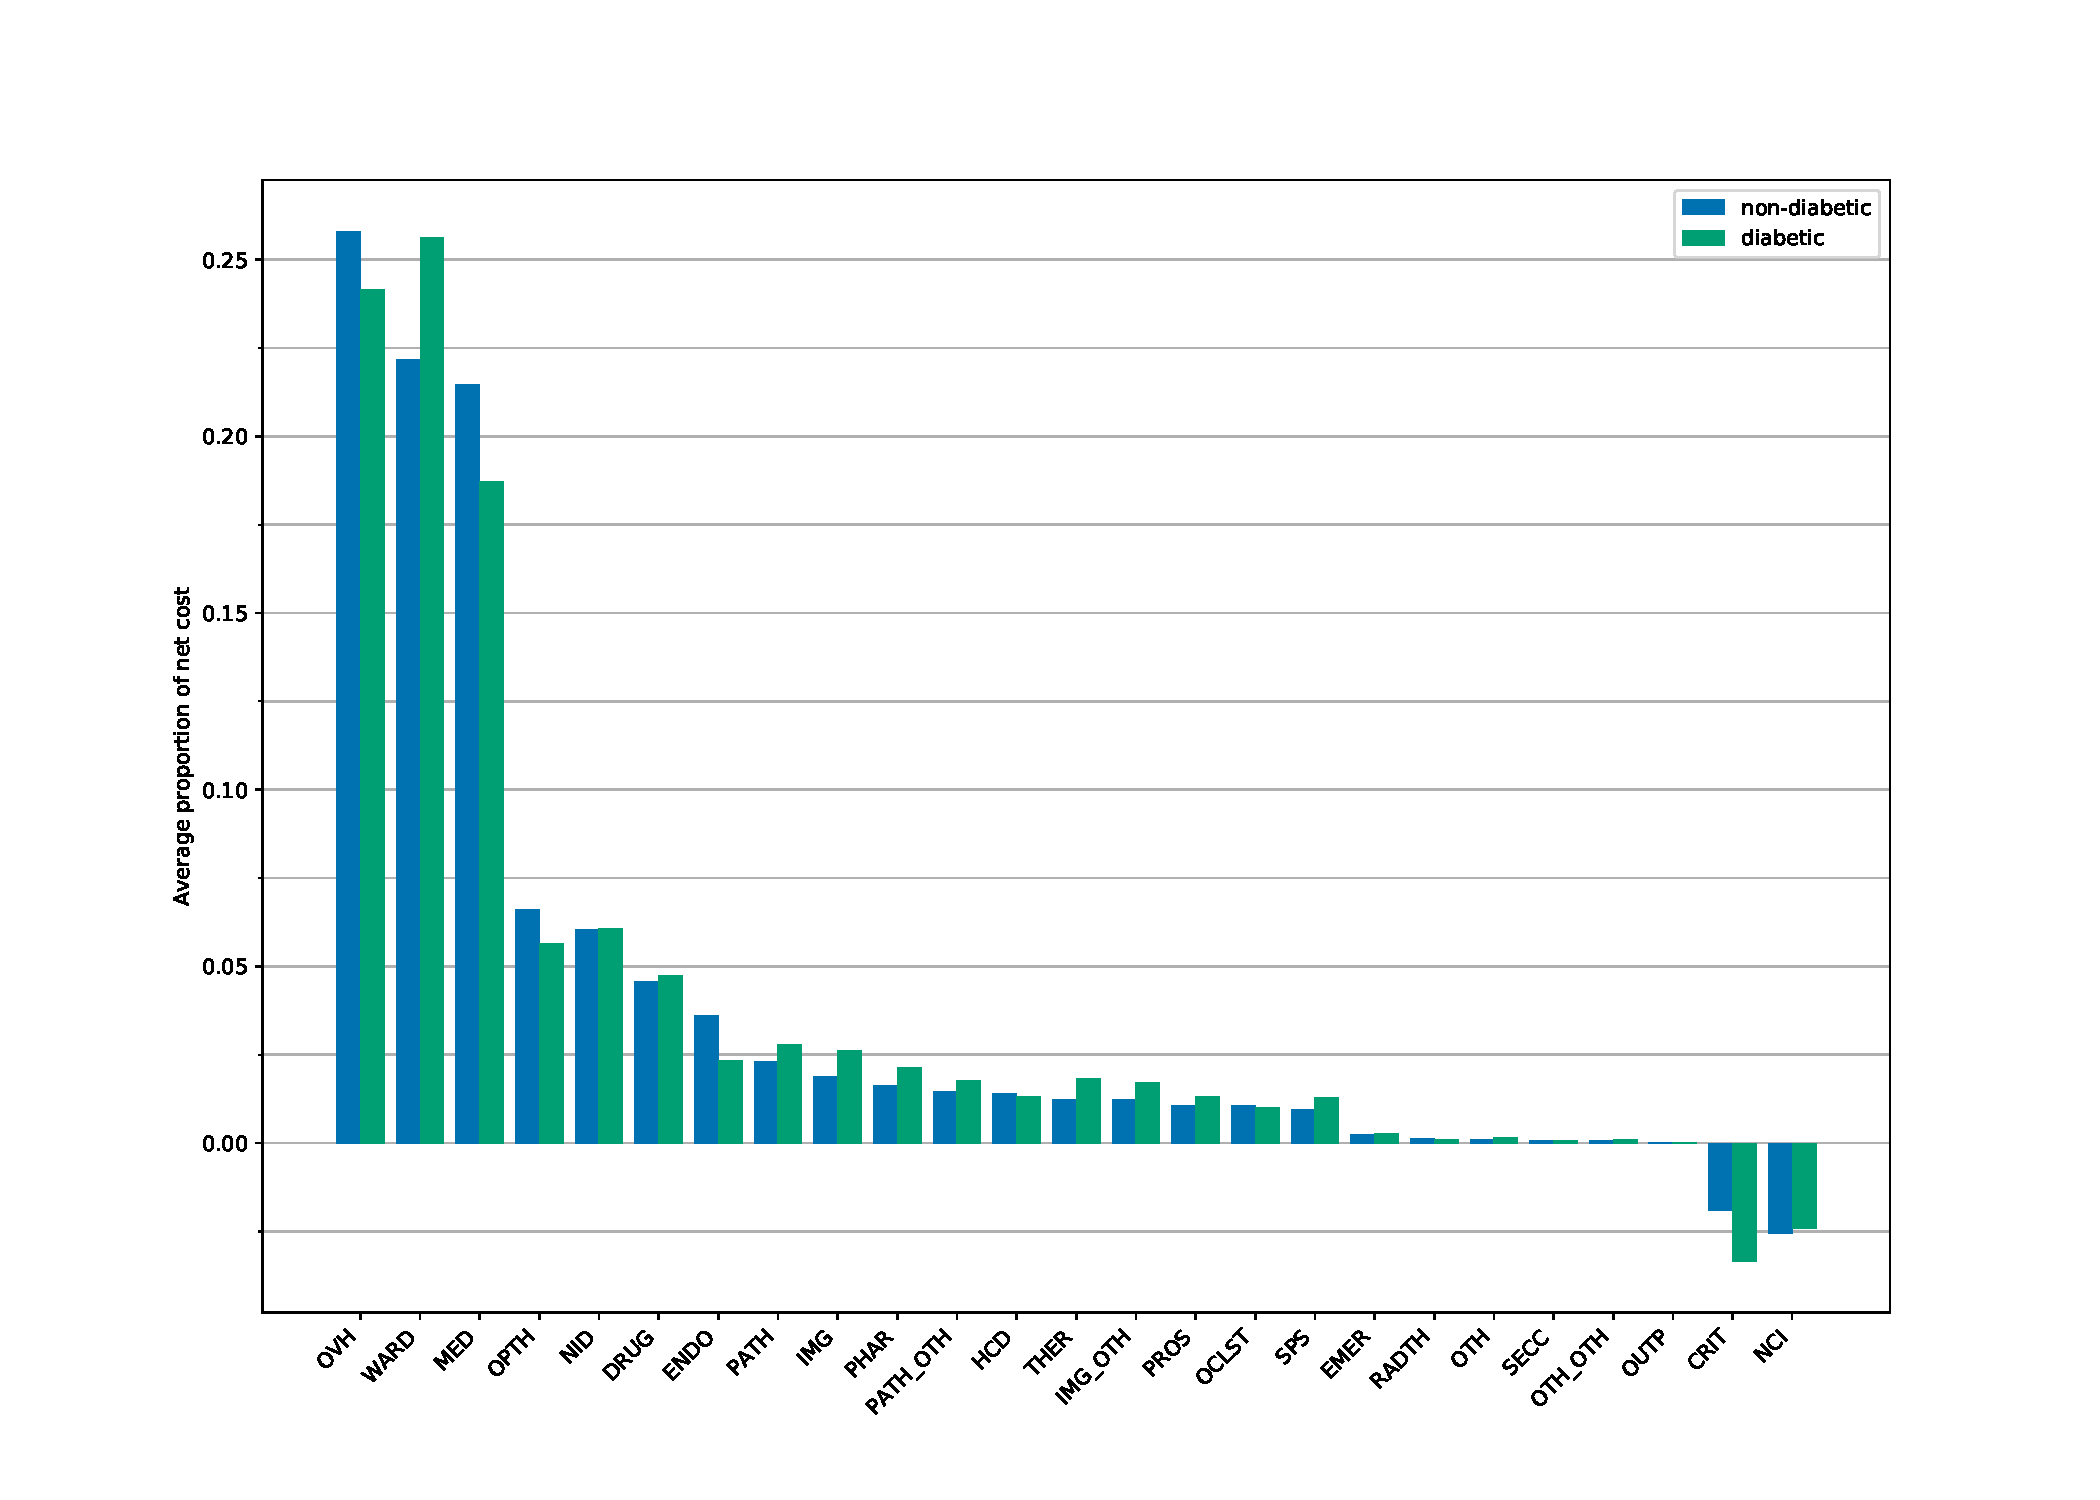
\includegraphics[width=\linewidth]{./img/diabetic_cost_contribution.pdf}
    \end{figure}
\end{frame}

\begin{frame}
    \frametitle{Correlation}

    \vspace{-15pt}
    \begin{figure}
        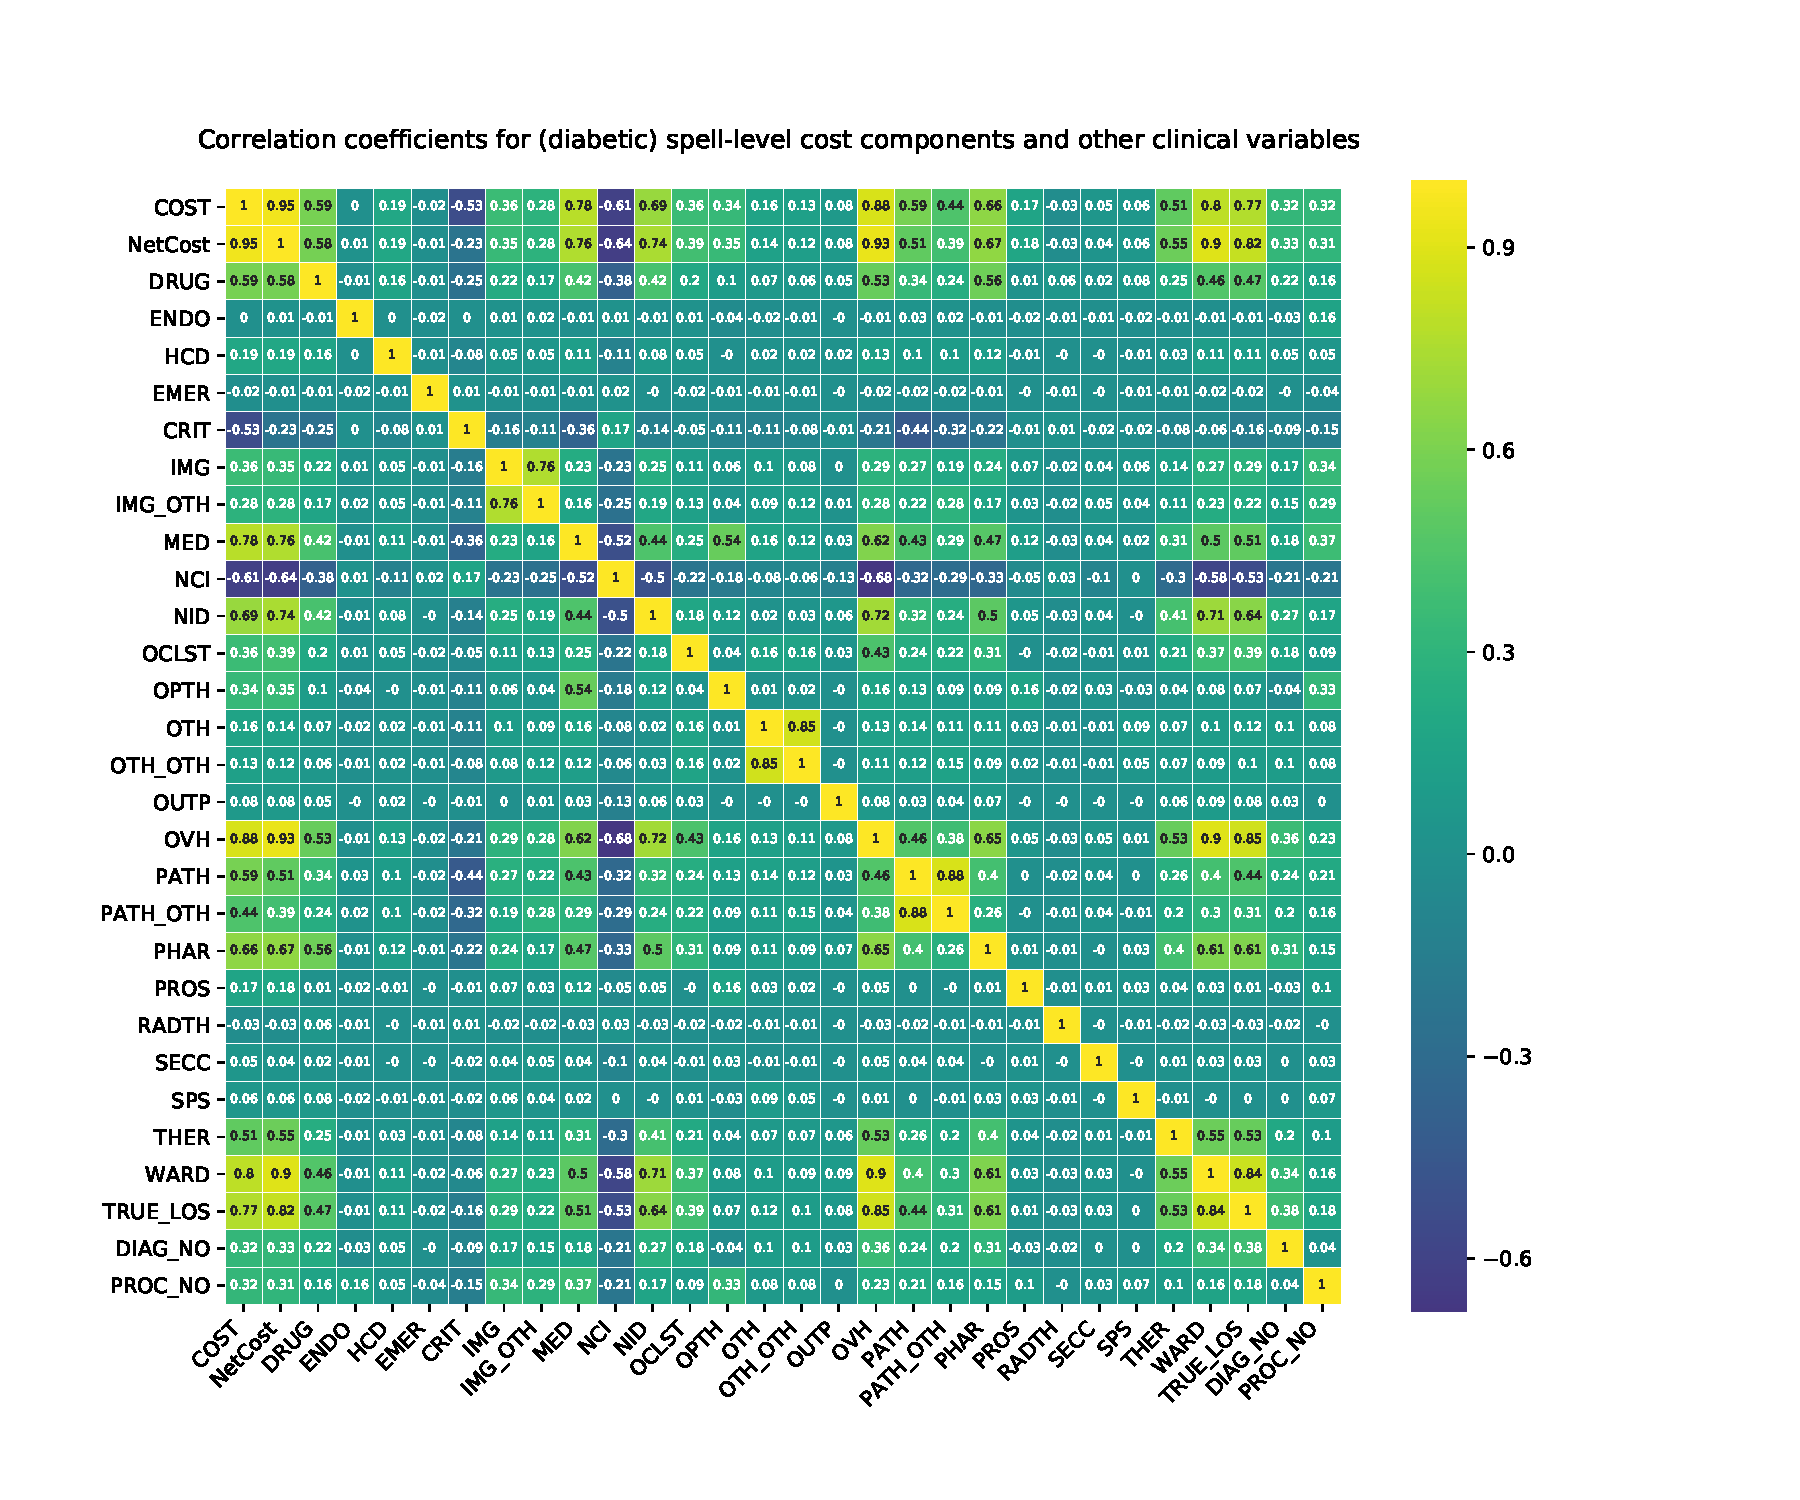
\includegraphics[width=\linewidth]{./img/diabetic_corr_heatmap.pdf}
    \end{figure}
\end{frame}

\begin{frame}
    \frametitle{Correlation (differences)}

    \vspace{-15pt}
    \begin{figure}
        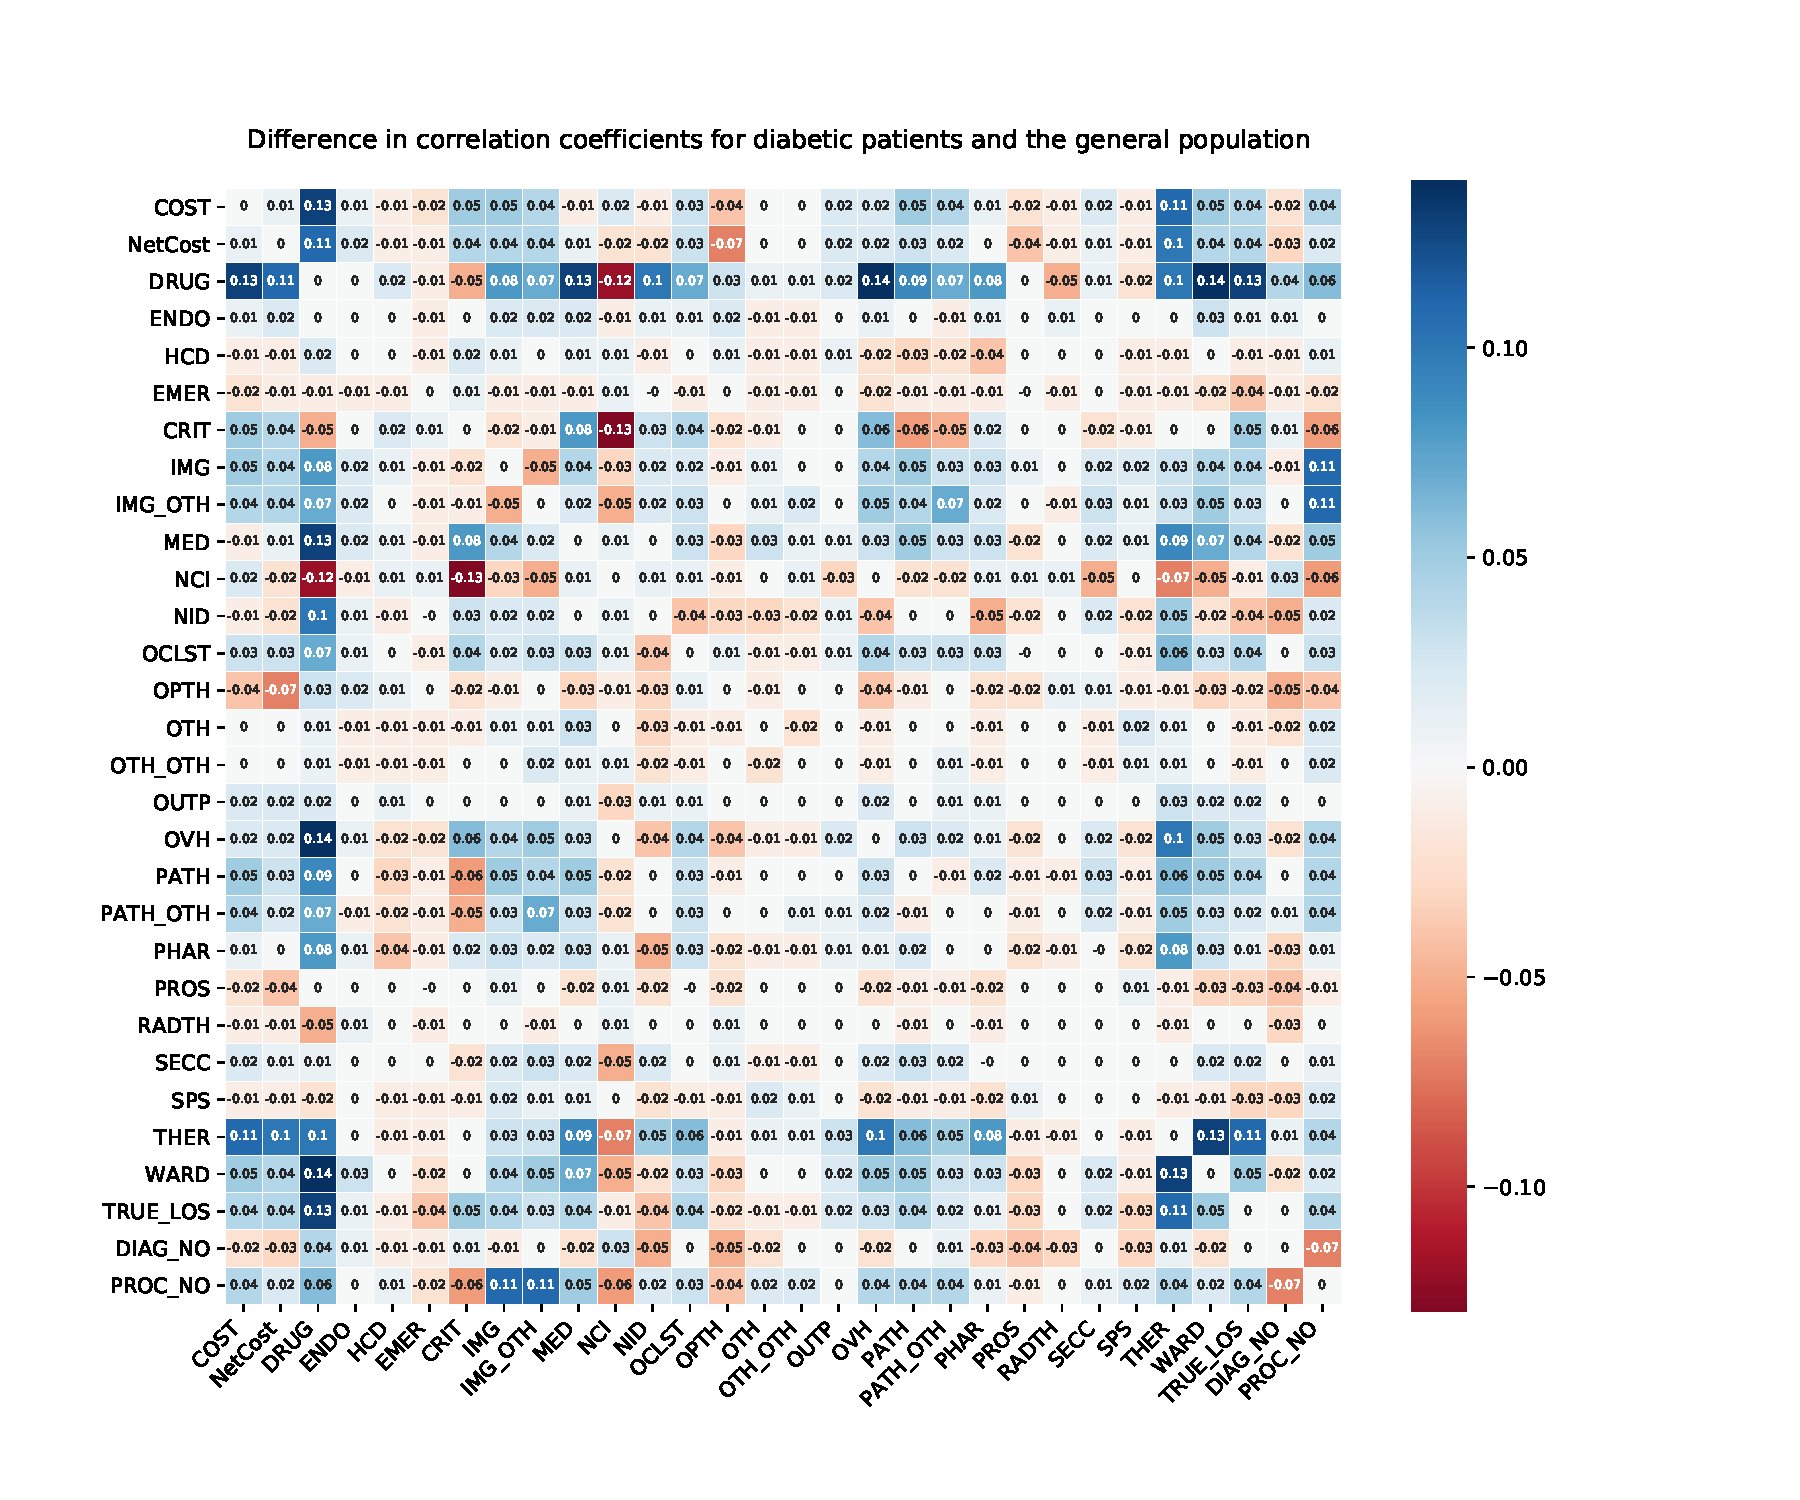
\includegraphics[width=\linewidth]{./img/differences_corr_heatmap.pdf}
    \end{figure}
\end{frame}

\begin{frame}
    \frametitle{Diabetic patient analysis}

    We will focus our definition of system `cost' on three measures:

    \pause%
    \begin{itemize}
        \item Proportion of total daily admissions
        \item Average length of stay given admission date
        \item Proportion of net costs spent given admission date
    \end{itemize}

    \pause%
    \vspace{10pt}
    These are indicators of resources used and resources necessary.

    \vspace{10pt}
    This grouping by admission date will lead to a degree of misrepresentation
    in our plots.

    \vspace{10pt}
    Allows us to investigate patterns developing over time.
\end{frame}

\begin{frame}
    \frametitle{Resource consumption}

    \begin{figure}
        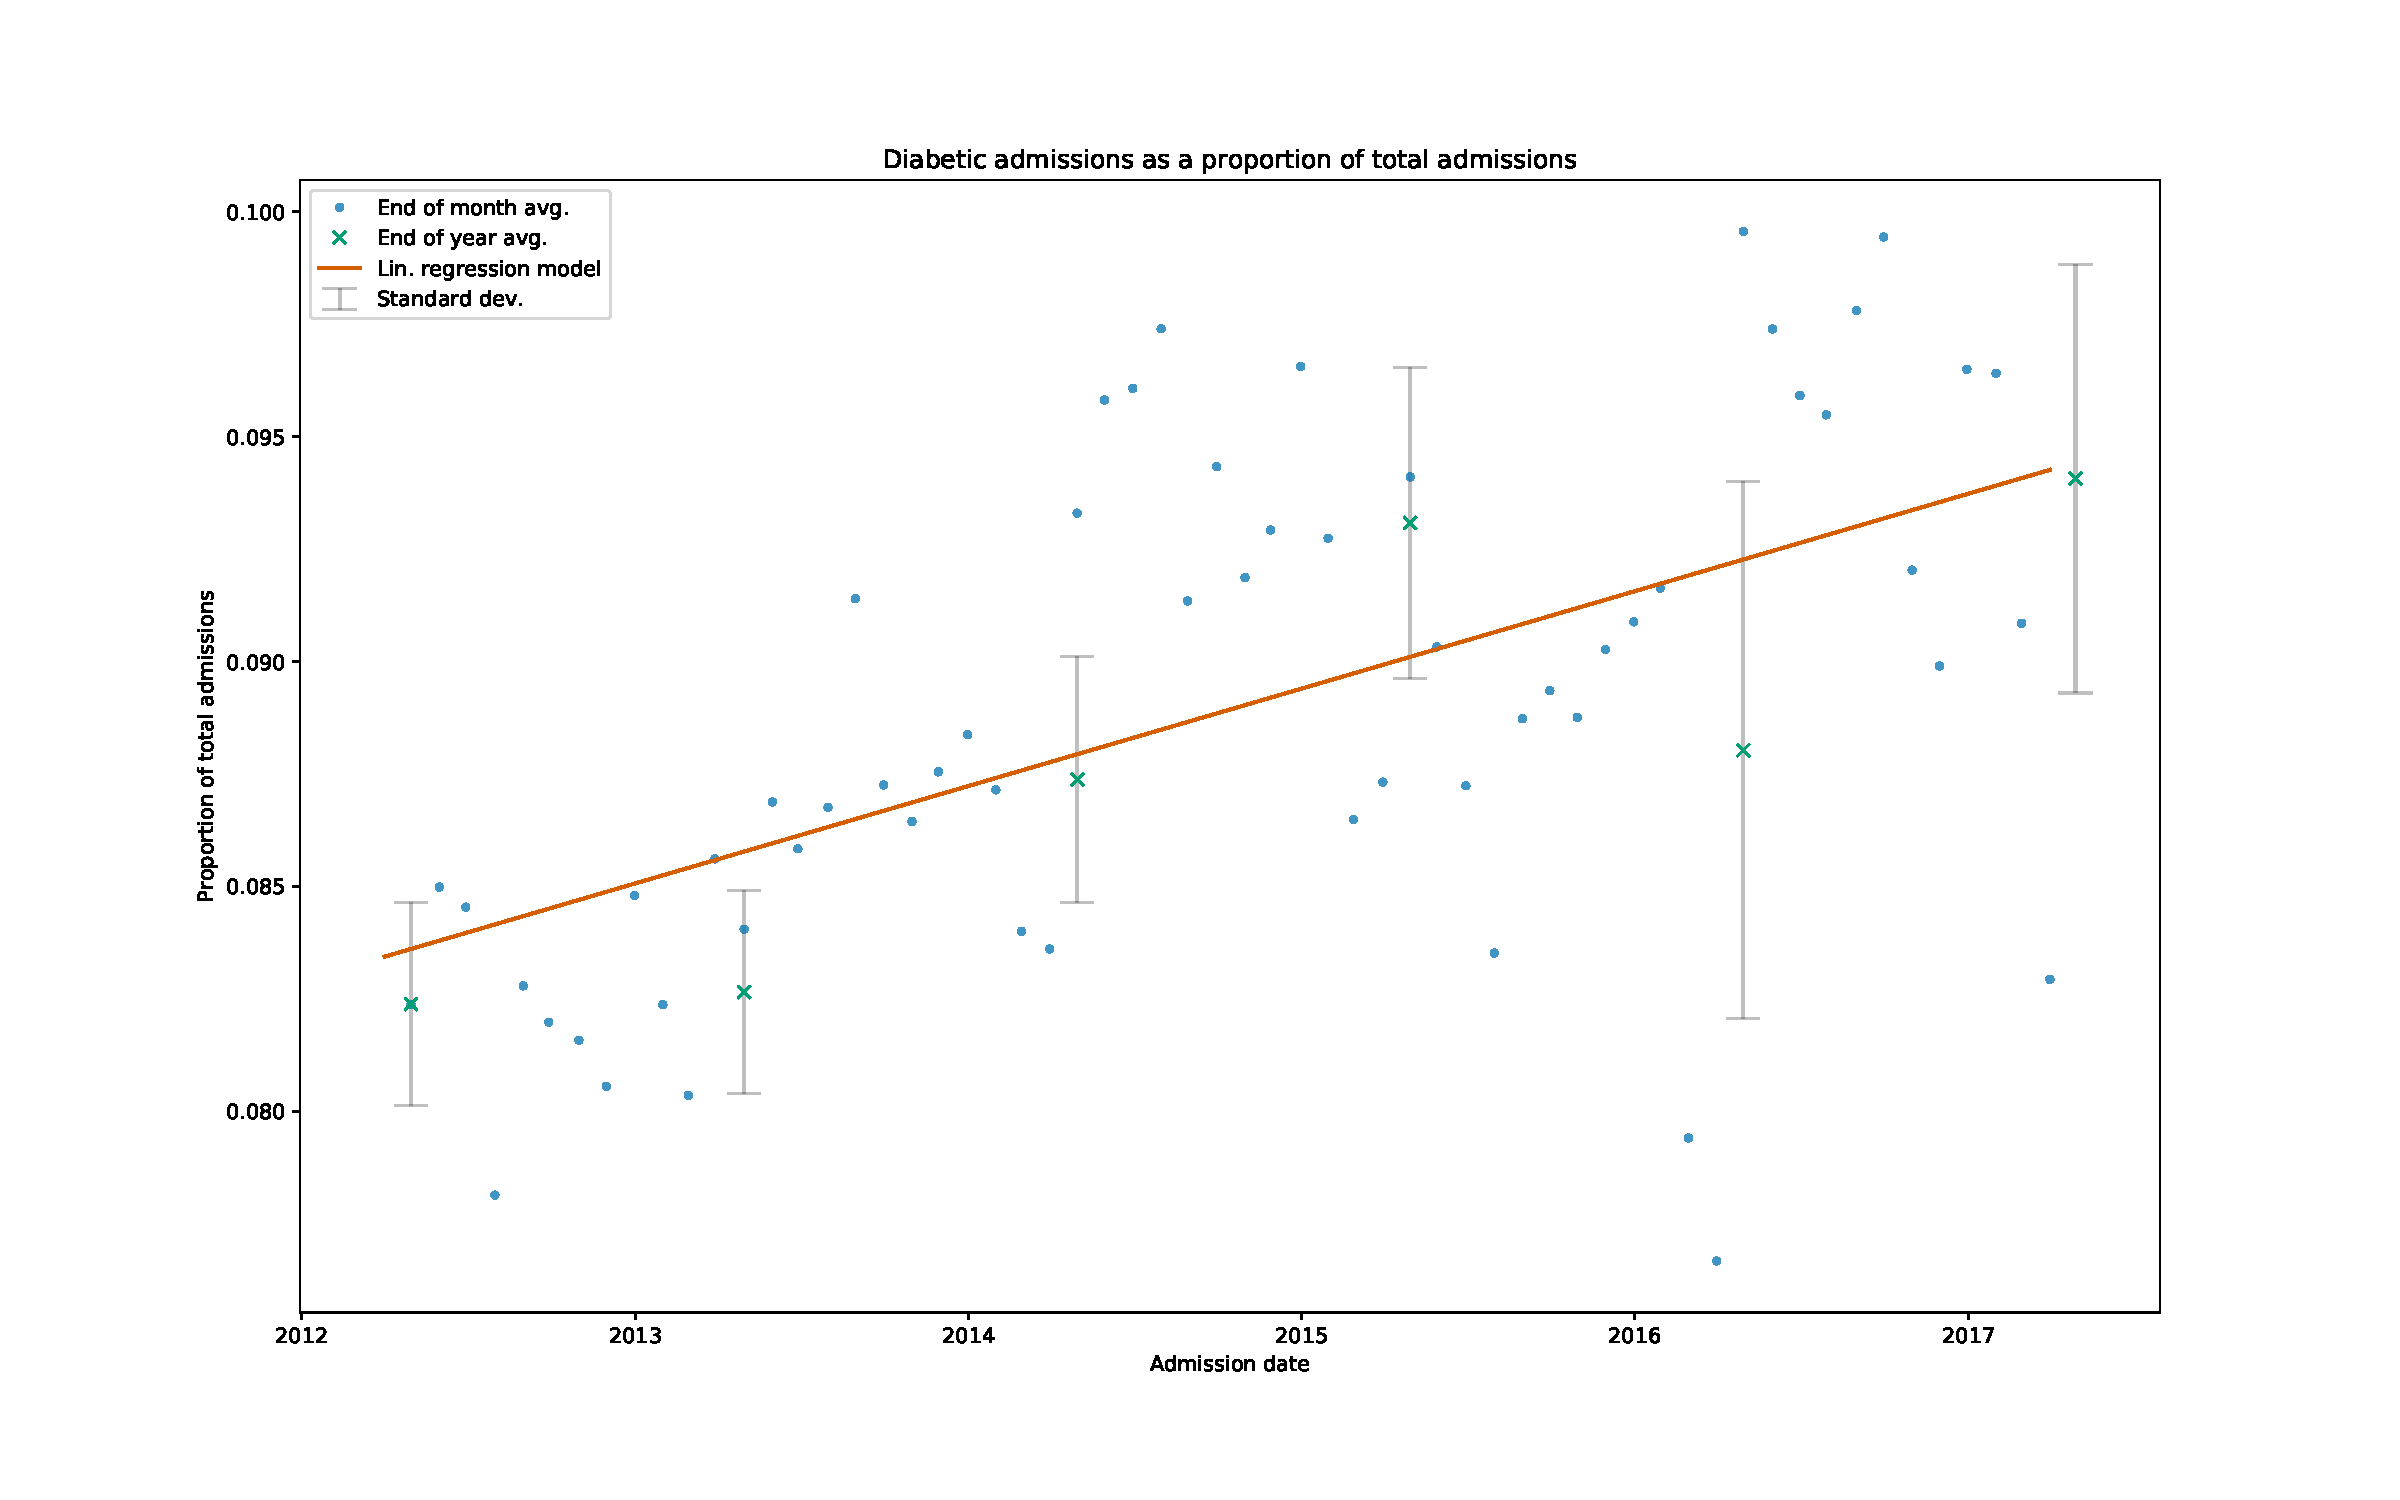
\includegraphics[width=\linewidth]{./img/diabetic_admissions.pdf}
    \end{figure}
\end{frame}

\begin{frame}
    \frametitle{Resource consumption}

    \begin{figure}
        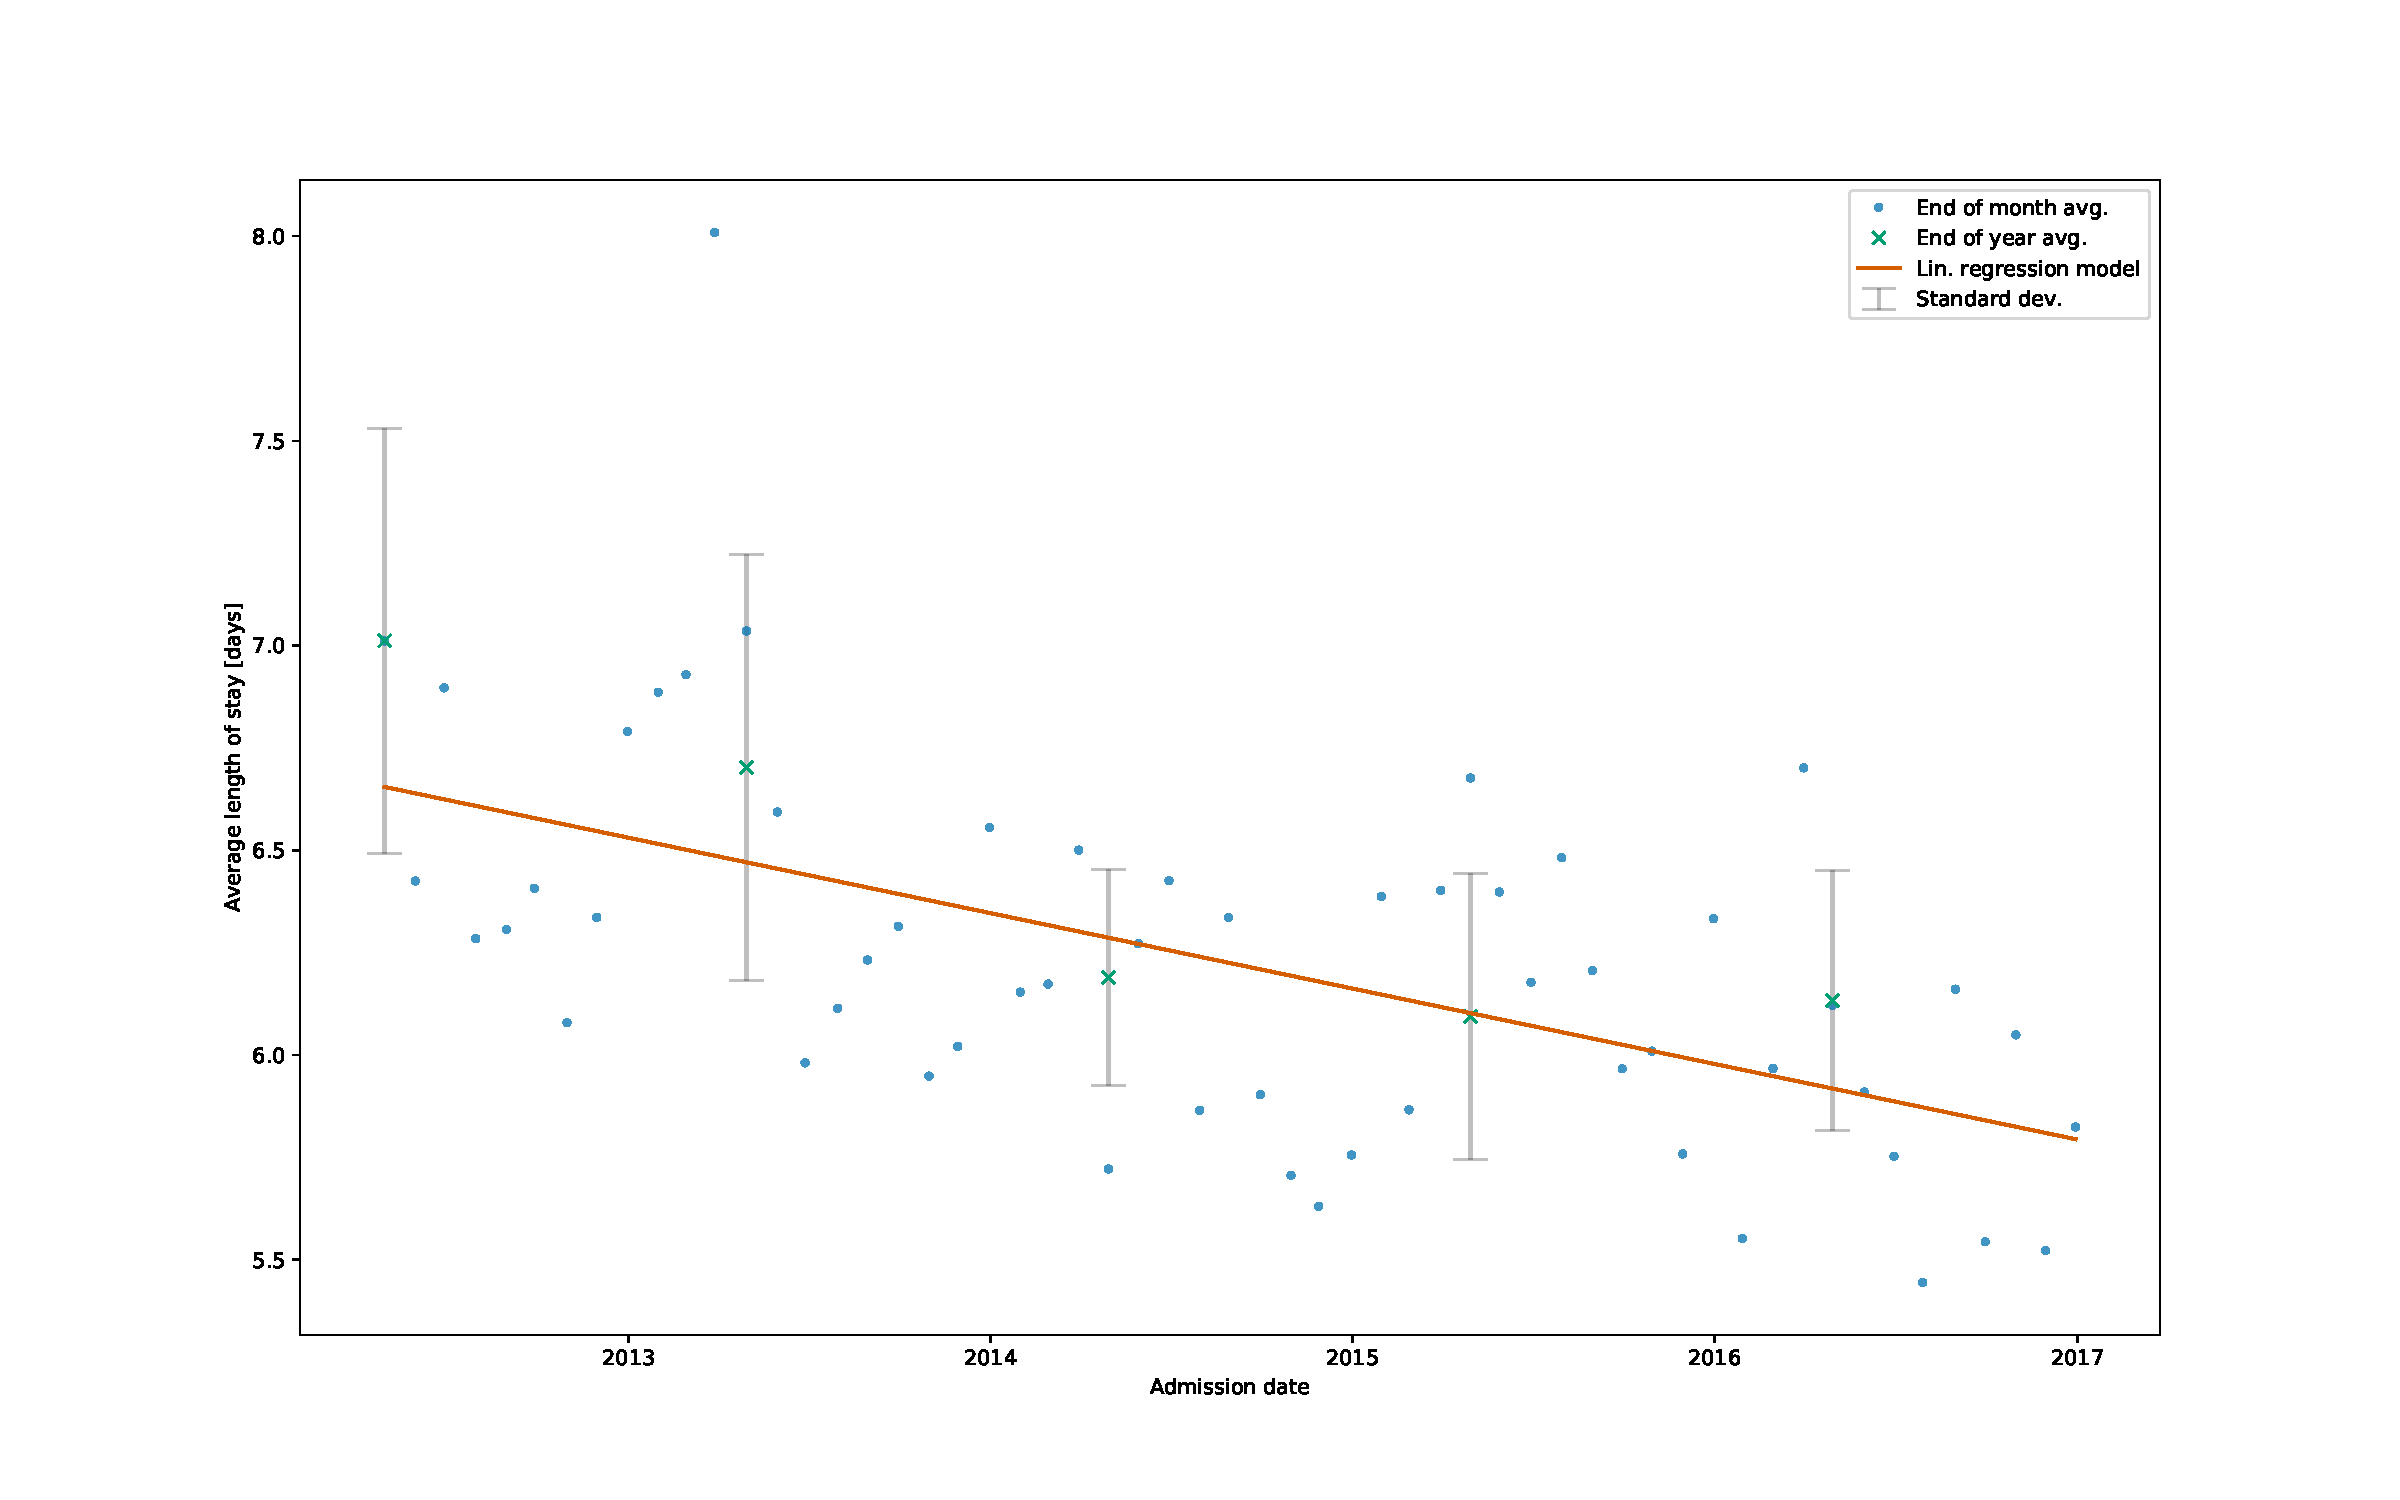
\includegraphics[width=\linewidth]{./img/diabetic_LOS_time.pdf}
    \end{figure}
\end{frame}

\begin{frame}
    \frametitle{Resource consumption}

    \begin{figure}
        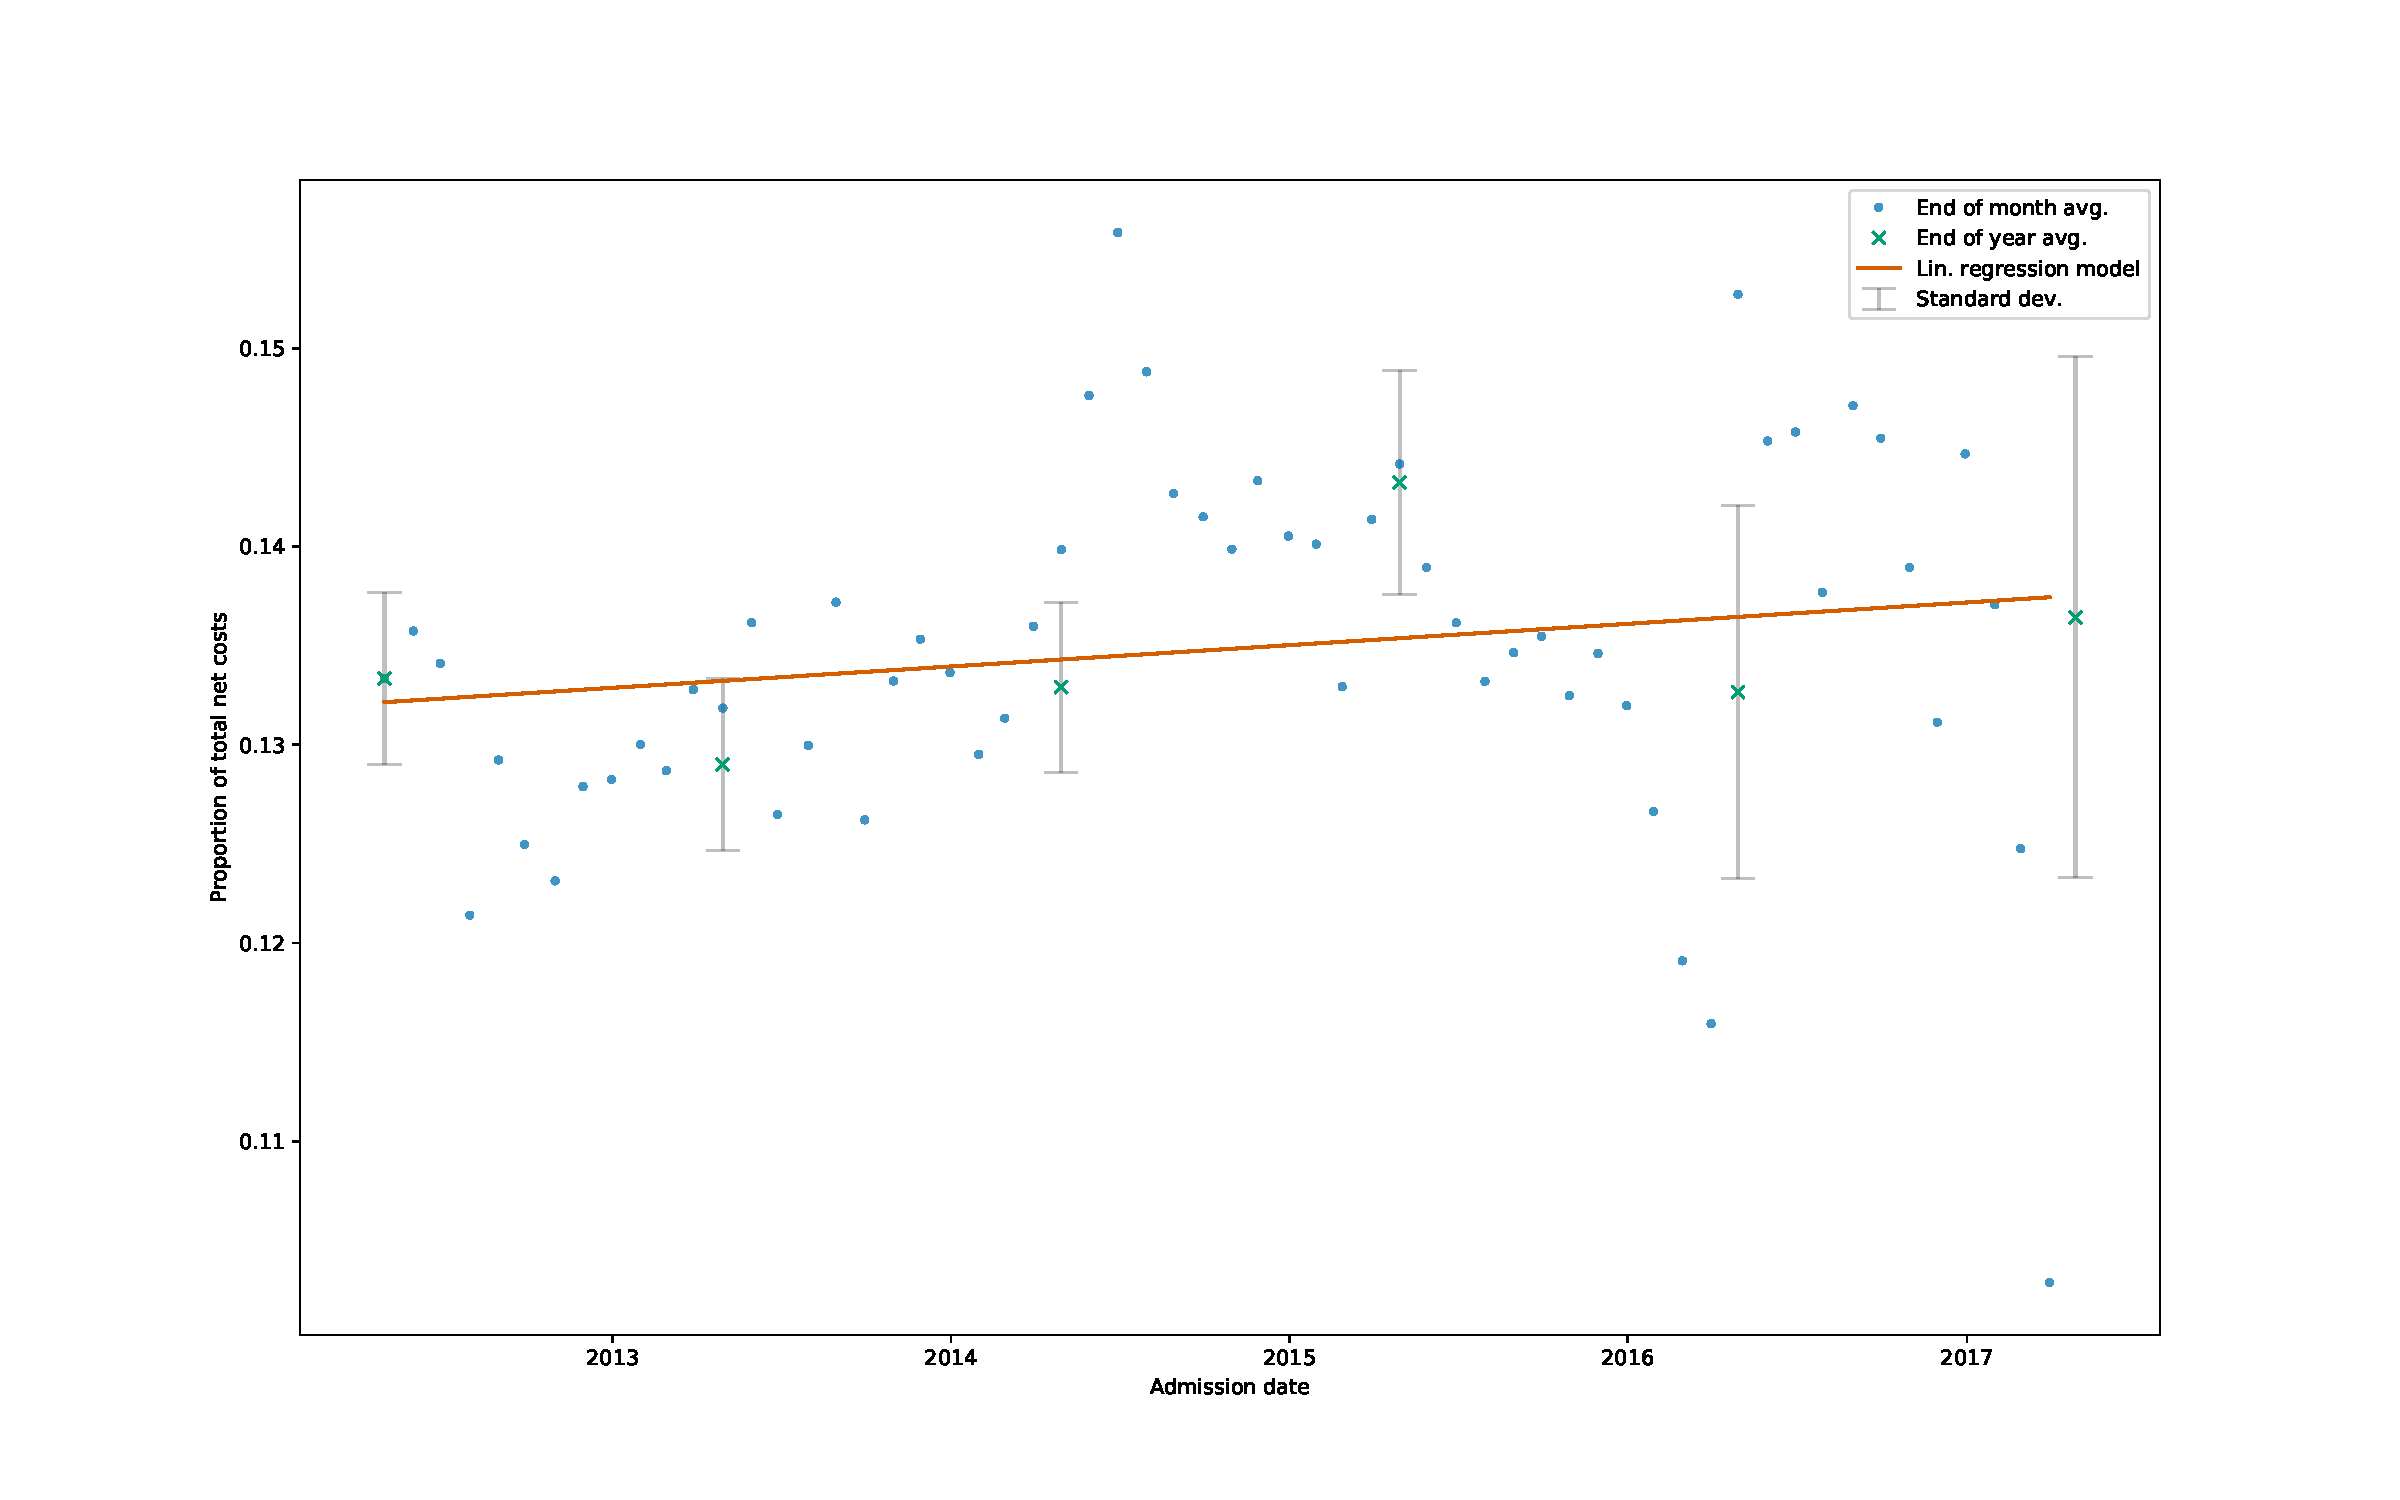
\includegraphics[width=\linewidth]
            {./img/diabetic_netcost_proportions.pdf}
    \end{figure}
\end{frame}

\begin{frame}
    \frametitle{Conclusions}

    \begin{itemize}
        \item Relative resource consumption by diabetic patients is consistent
        \item Cost components are less variant than \-- and are comparable in
            their distribution to \-- non-diabetic patients
    \end{itemize}
\end{frame}

\section{Moving forward}

\begin{frame}
    \frametitle{Moving forward}
    \begin{itemize}
        \pause%
        \item Resource consumption metric
        \pause%
        \item Perform clustering analysis to find inherent slices in the data
        \pause%
        \item Incorporate external data
        \begin{itemize}
            \item Decode GP practice codes for GeoPandas
            \item Socio-economic analysis based on deprivation and geography
            \item Temperature-based analysis
        \end{itemize}
        \pause%
        \item Severity and comorbidity analysis
        \begin{itemize}
            \item Average severity of secondary conditions given some primary
                condition
            \item Using the comorbidity index as a class label in some
                predictive analysis
        \end{itemize}
    \end{itemize}
\end{frame}

\end{document}

\documentclass{beamer}

\usepackage{graphicx}

\title{An exploratory analysis of patient episode data}
\author{Henry Wilde}
\institute{Cardiff University School of Mathematics}

\usetheme{Hannover}
\usecolortheme{seahorse}
\begin{document}

\begin{frame}
\titlepage%
\end{frame}

\begin{frame}
\frametitle{Outline}
\tableofcontents
\end{frame}

\section{Motivation}

\begin{frame}
\frametitle{Motivation}

\begin{itemize}
    \item Observe and understand cost variation
    \item Identify important slices in the data
    \item Develop methods for examining slices of the data
    \item Analyse their impact on costs and resource consumption
\end{itemize}
\end{frame}

\section{Getting to know the data}

\subsection{Structure and origin}
\begin{frame}
    \frametitle{Structure and origin}

    \pause%
    All data is provided by the Cwm Taf University Health Board.
    \vspace{10pt}

    \pause%
    We have:
    \begin{itemize}
        \item 2,447,299 patient episodes
        \item 1,946,545 patient spells
        \item 865,421 individual patients
    \end{itemize}
    \vspace{10pt}

    \pause%
    Each row is made up of roughly 250 attributes, including:
    \begin{itemize}
        \pause%
        \item personal identifiers and demographic information
        \pause%
        \item condition and treatment indicators (HRG, OPCS4, ICD10)
        \pause%
        \item other clinical references
        \pause%
        \item cost components
    \end{itemize}
\end{frame}

\subsection{Summative analysis}
\begin{frame}
    \frametitle{Summative analysis}

    \begin{itemize}
        \pause%
        \item Our data is skewed towards low-cost, short-stay episodes
        \pause%
        \item This extends to the spell level with largely one or two-time
            visits from patients
        \pause%
        \item Long and heavy tails are present in our costs and lengths of stay
    \end{itemize}
\end{frame}

\begin{frame}
    \frametitle{Number of spells}

    \begin{figure}
        \begin{minipage}{\linewidth}
            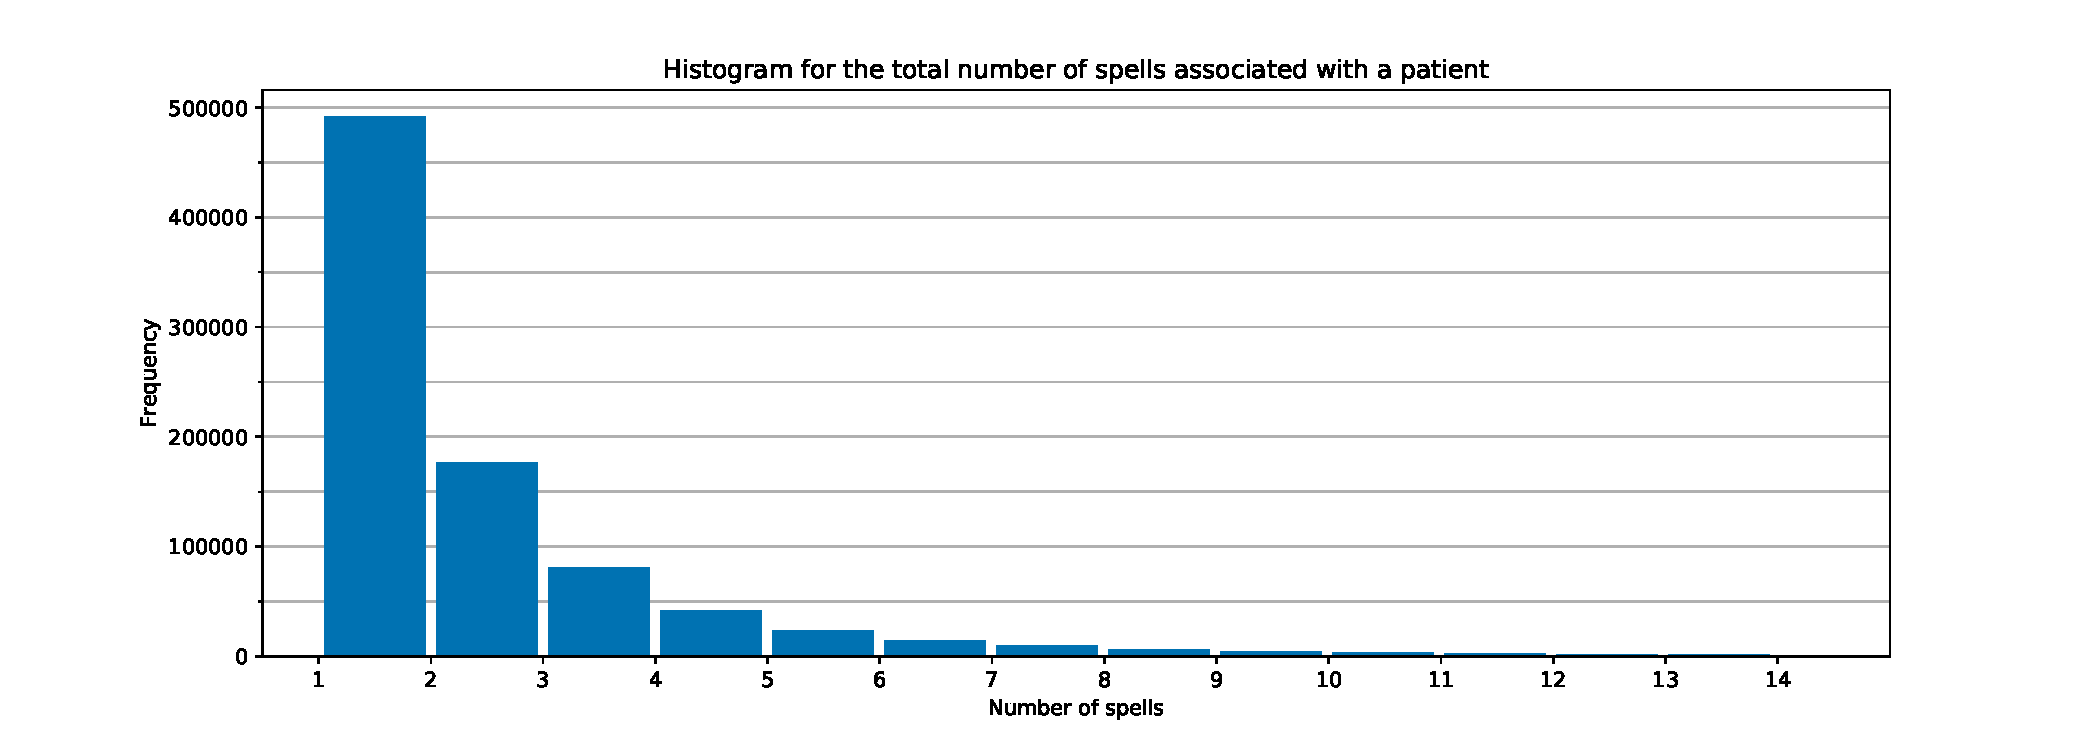
\includegraphics[width=\linewidth]{./img/no_spells_freq_hist.pdf}
        \end{minipage}
        \begin{minipage}{\linewidth}
            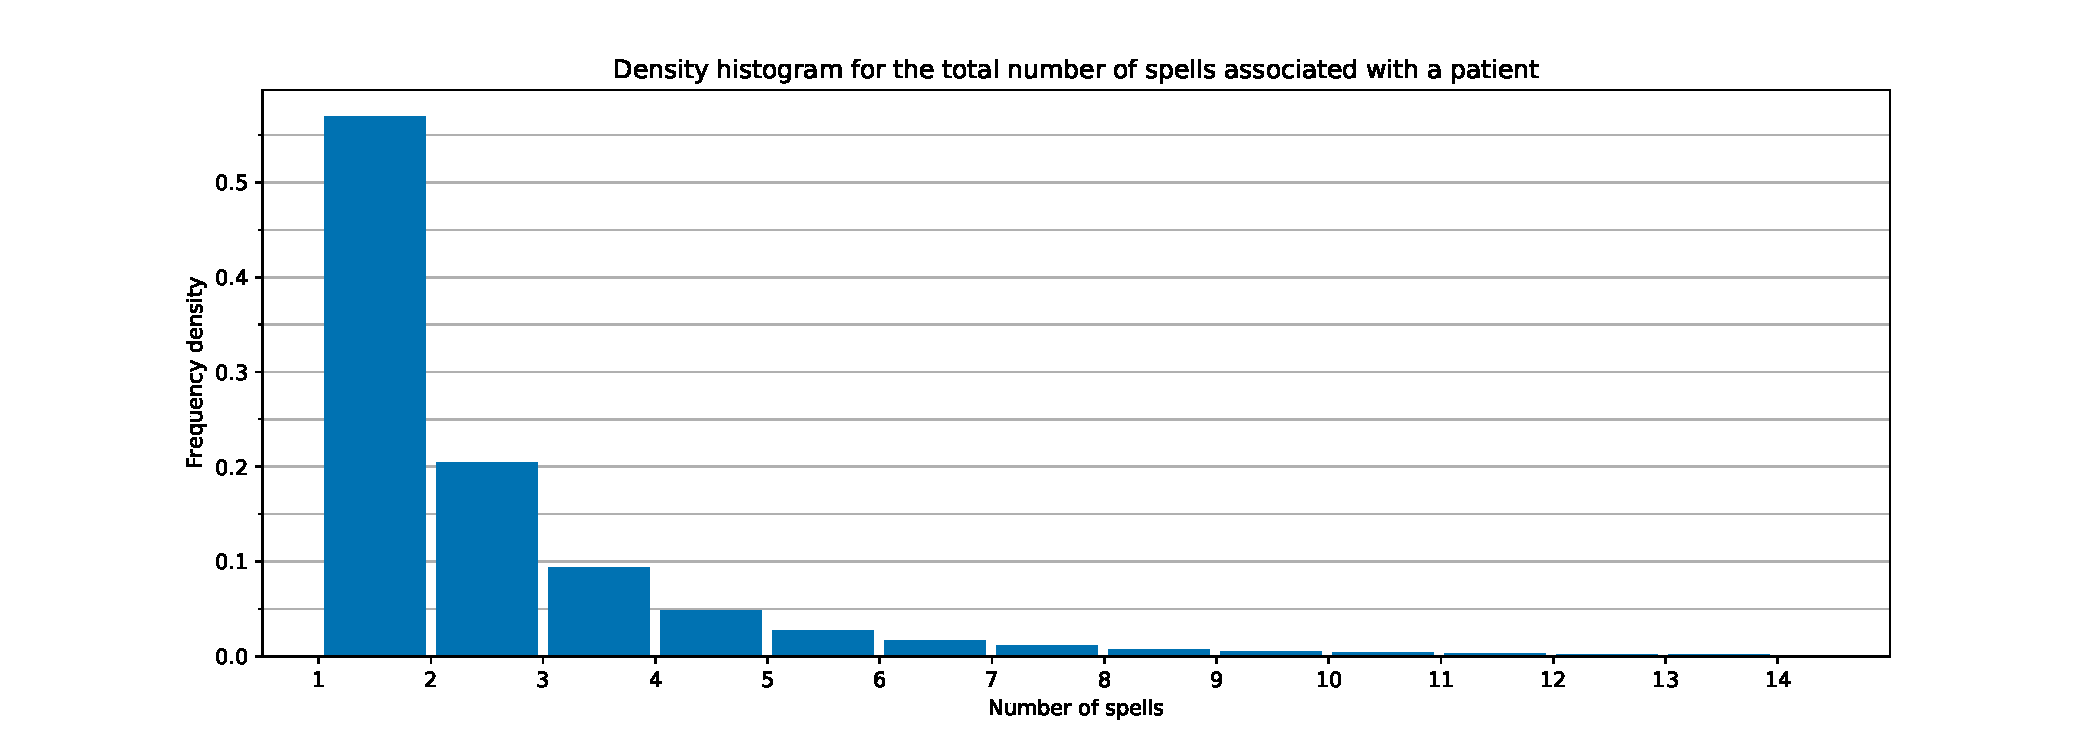
\includegraphics[width=\linewidth]{./img/no_spells_density_hist.pdf}
        \end{minipage}
    \end{figure}
\end{frame}

\begin{frame}
    \frametitle{Length of stay (spell-wise)}

    \begin{figure}
        \begin{minipage}{\linewidth}
            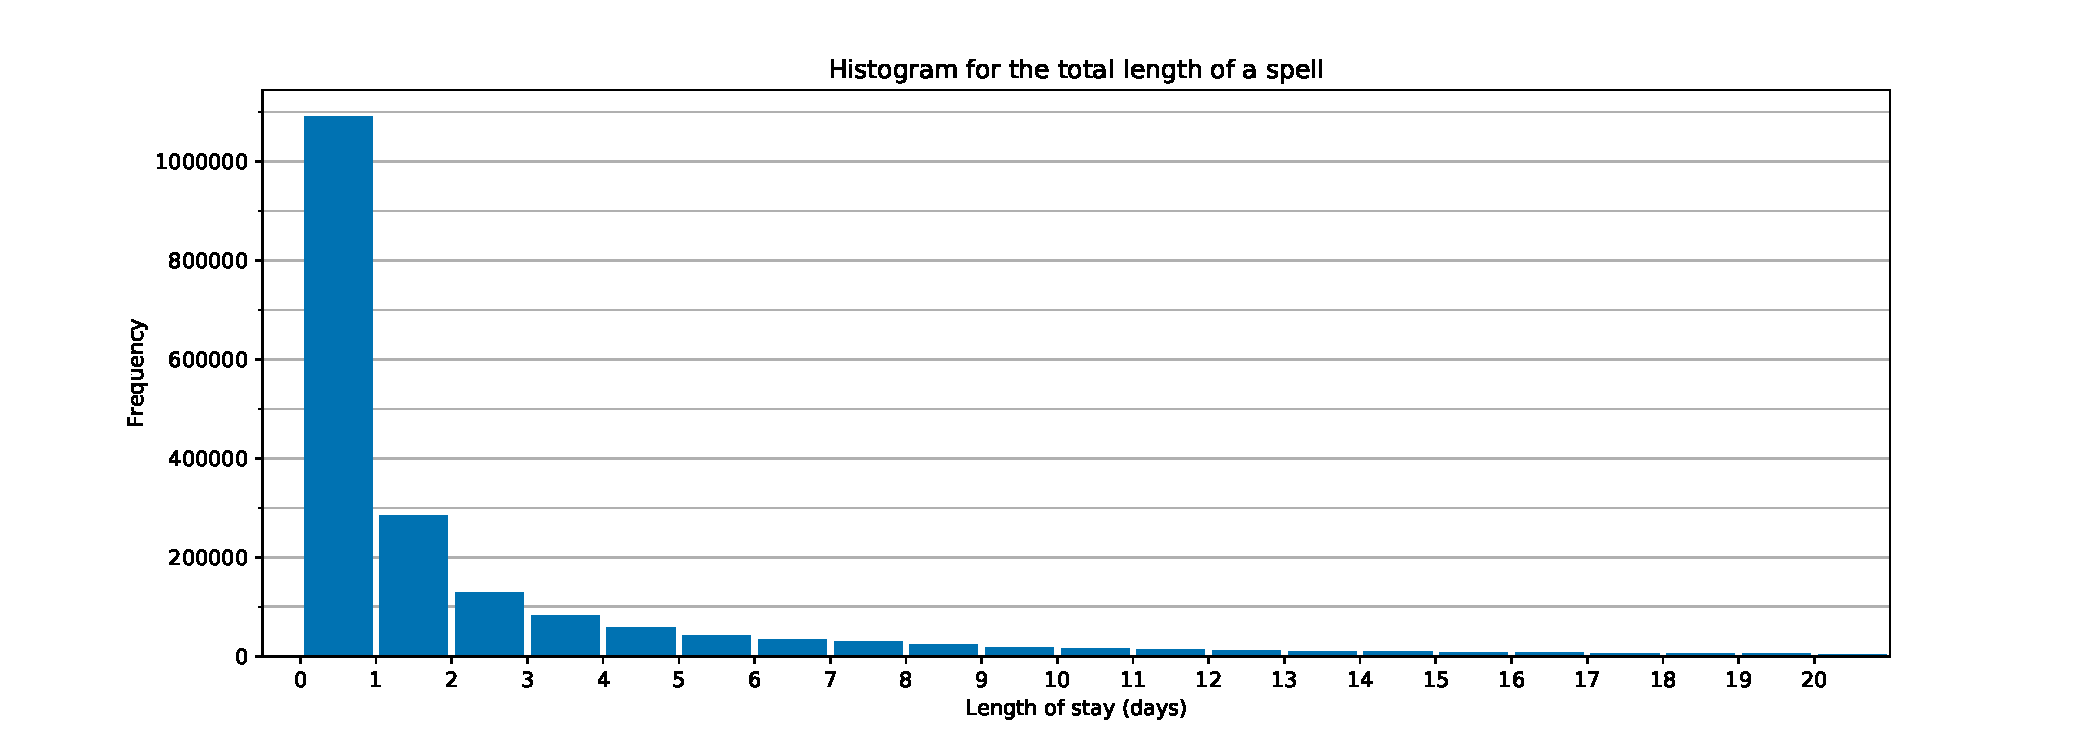
\includegraphics[width=\linewidth]{./img/LOS_freq_hist.pdf}
        \end{minipage}
        \begin{minipage}{\linewidth}
            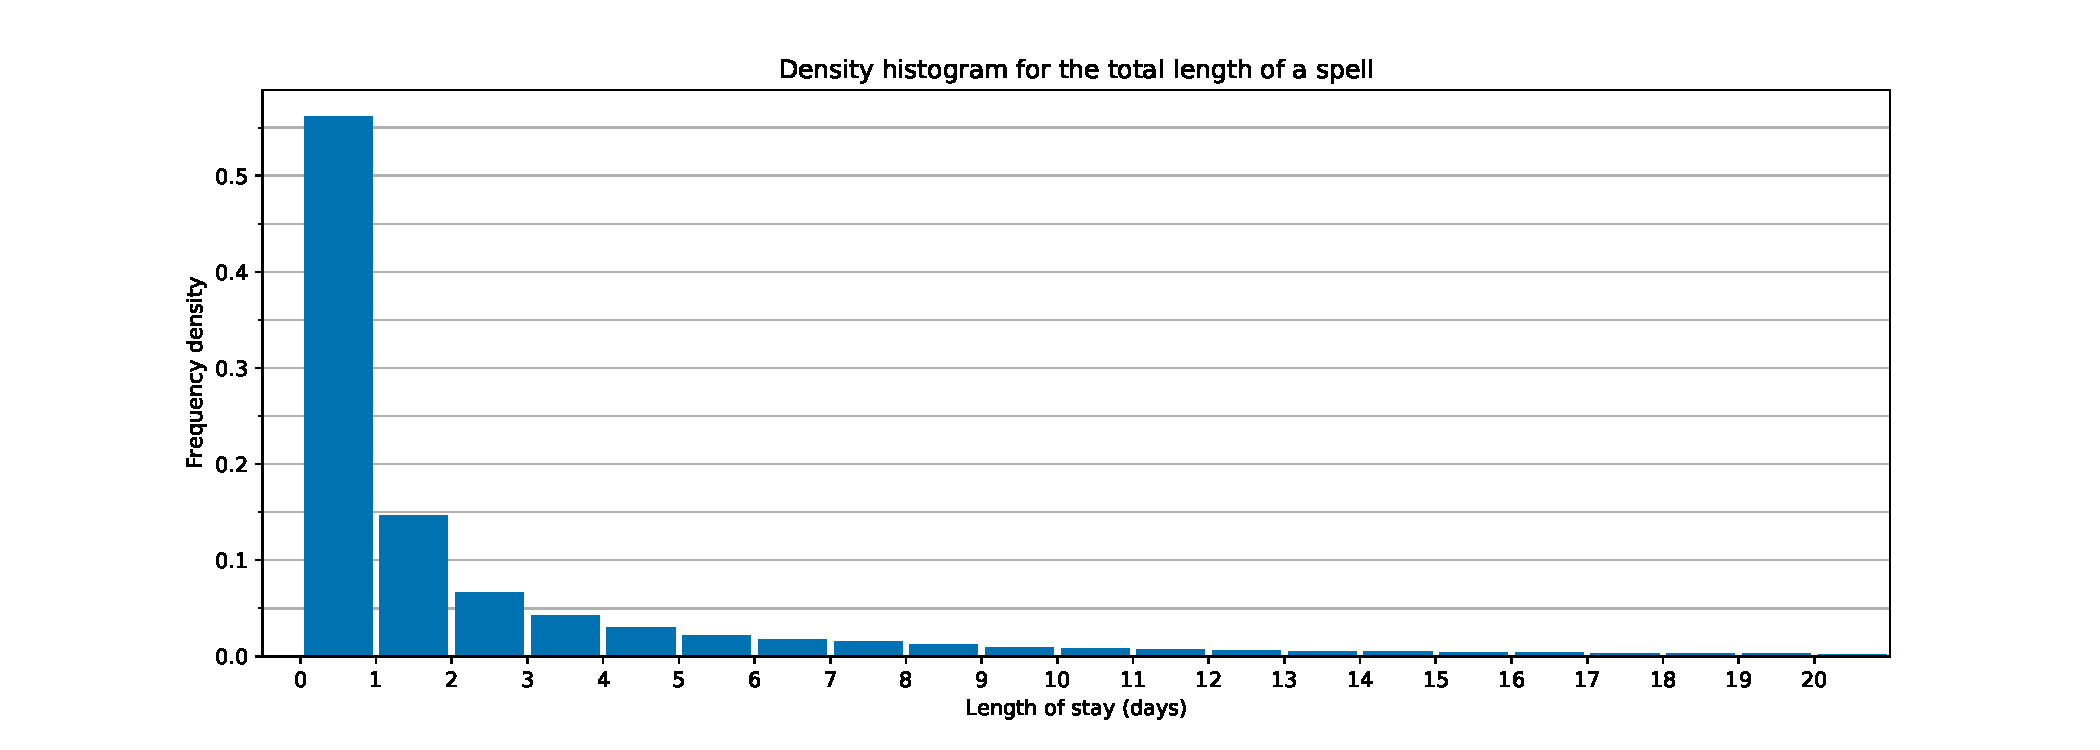
\includegraphics[width=\linewidth]{./img/LOS_density_hist.pdf}
        \end{minipage}
    \end{figure}
\end{frame}

\begin{frame}
    \frametitle{Net cost}

    \begin{figure}
        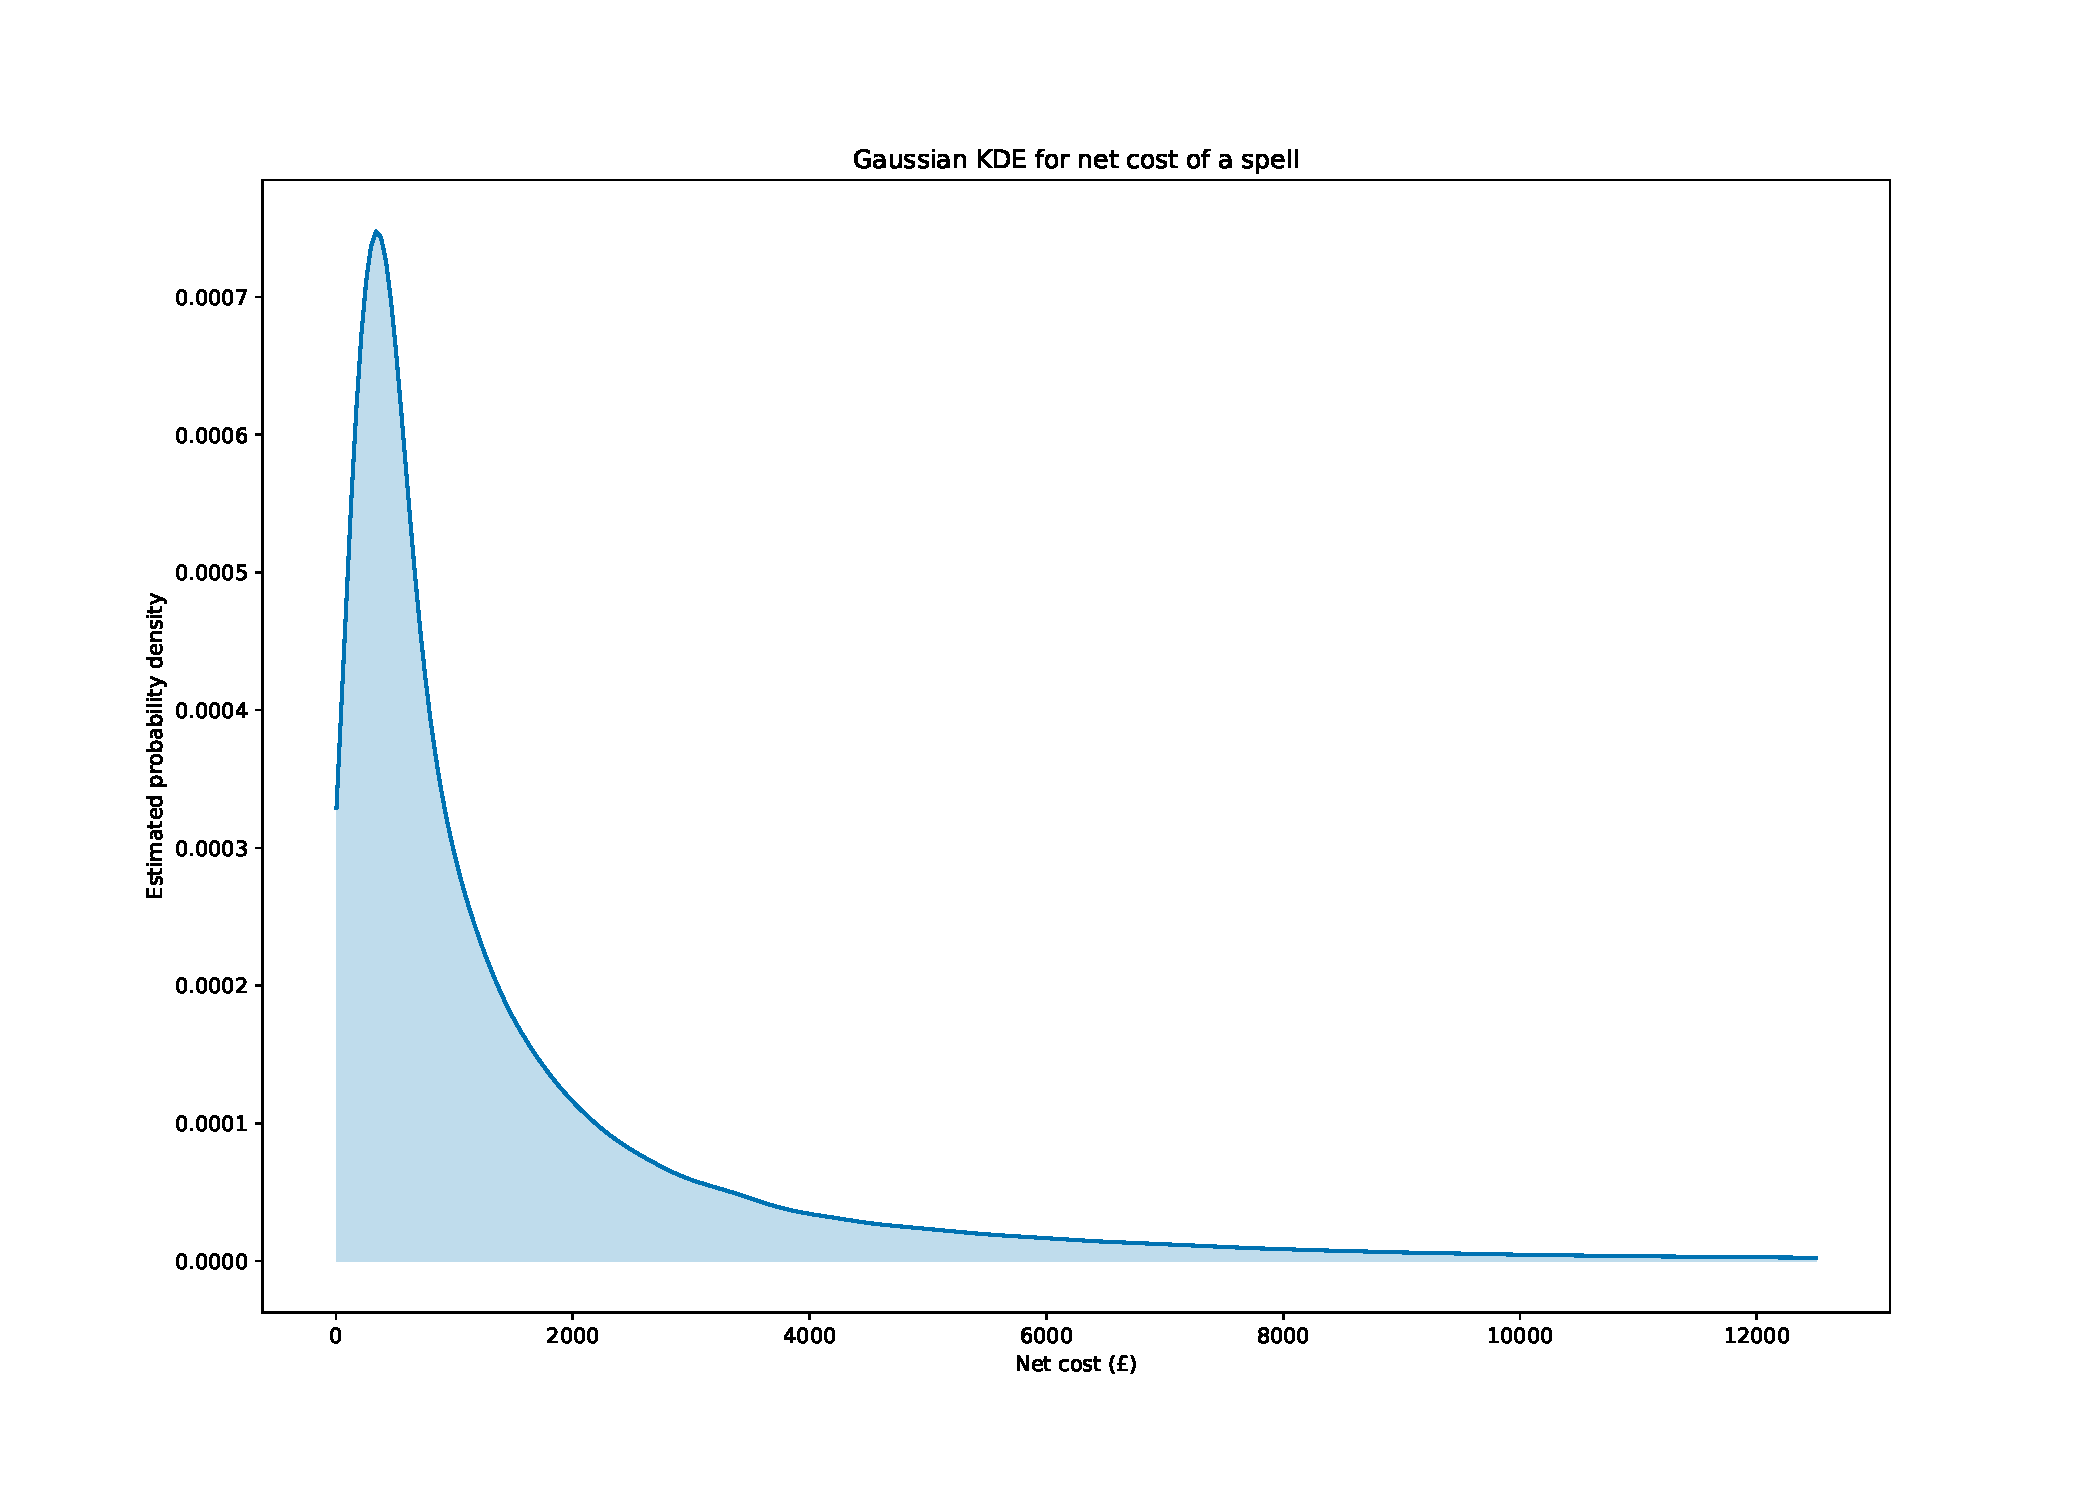
\includegraphics[width=\linewidth]{./img/netcost_kde.pdf}
    \end{figure}
\end{frame}

\begin{frame}
    \frametitle{Summative analysis}

    Other areas of interest to us are:
    \begin{itemize}
        \item Other clinical measures
        \item Demographic variables
        \item Interactions between variables
    \end{itemize}
\end{frame}

\begin{frame}
    \frametitle{Clinical variables}

    We will investigate:
    \begin{itemize}
        \item the number of diagnoses
        \item the number of procedures
    \end{itemize}

    \pause%
    These contribute to comorbidity rates and presumably costs.
\end{frame}

\begin{frame}
    \frametitle{Number of diagnoses}
   
    \begin{figure}
        \begin{minipage}{\linewidth}
            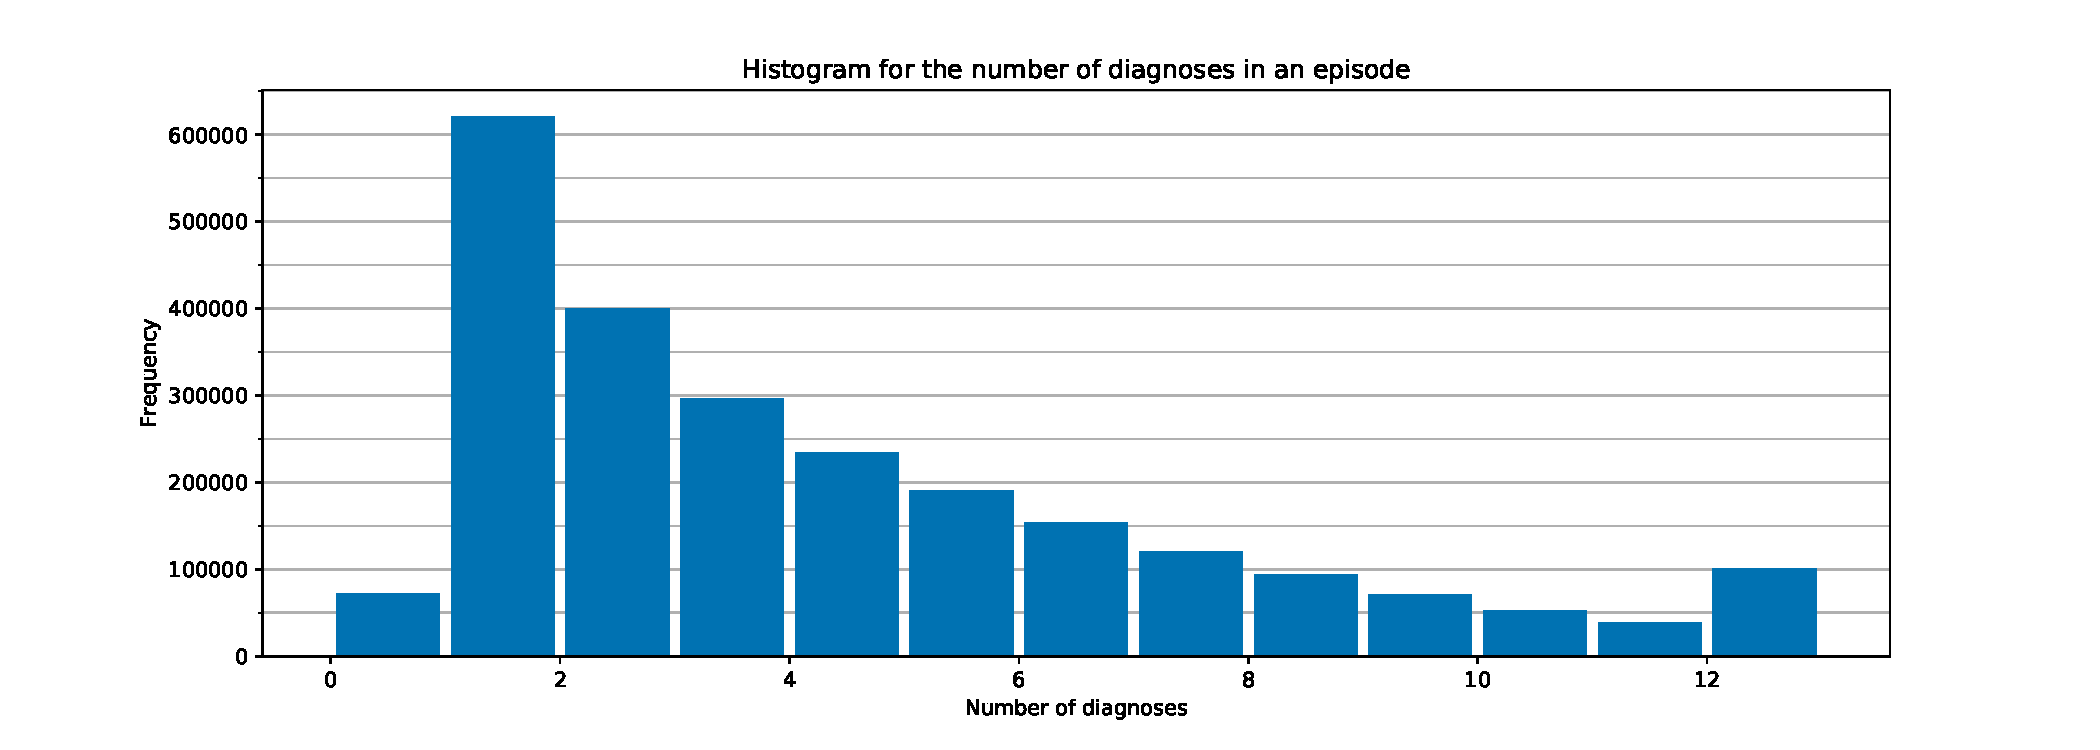
\includegraphics[width=\linewidth]{./img/diag_no_freq_hist.pdf}
        \end{minipage}
        \begin{minipage}{\linewidth}
            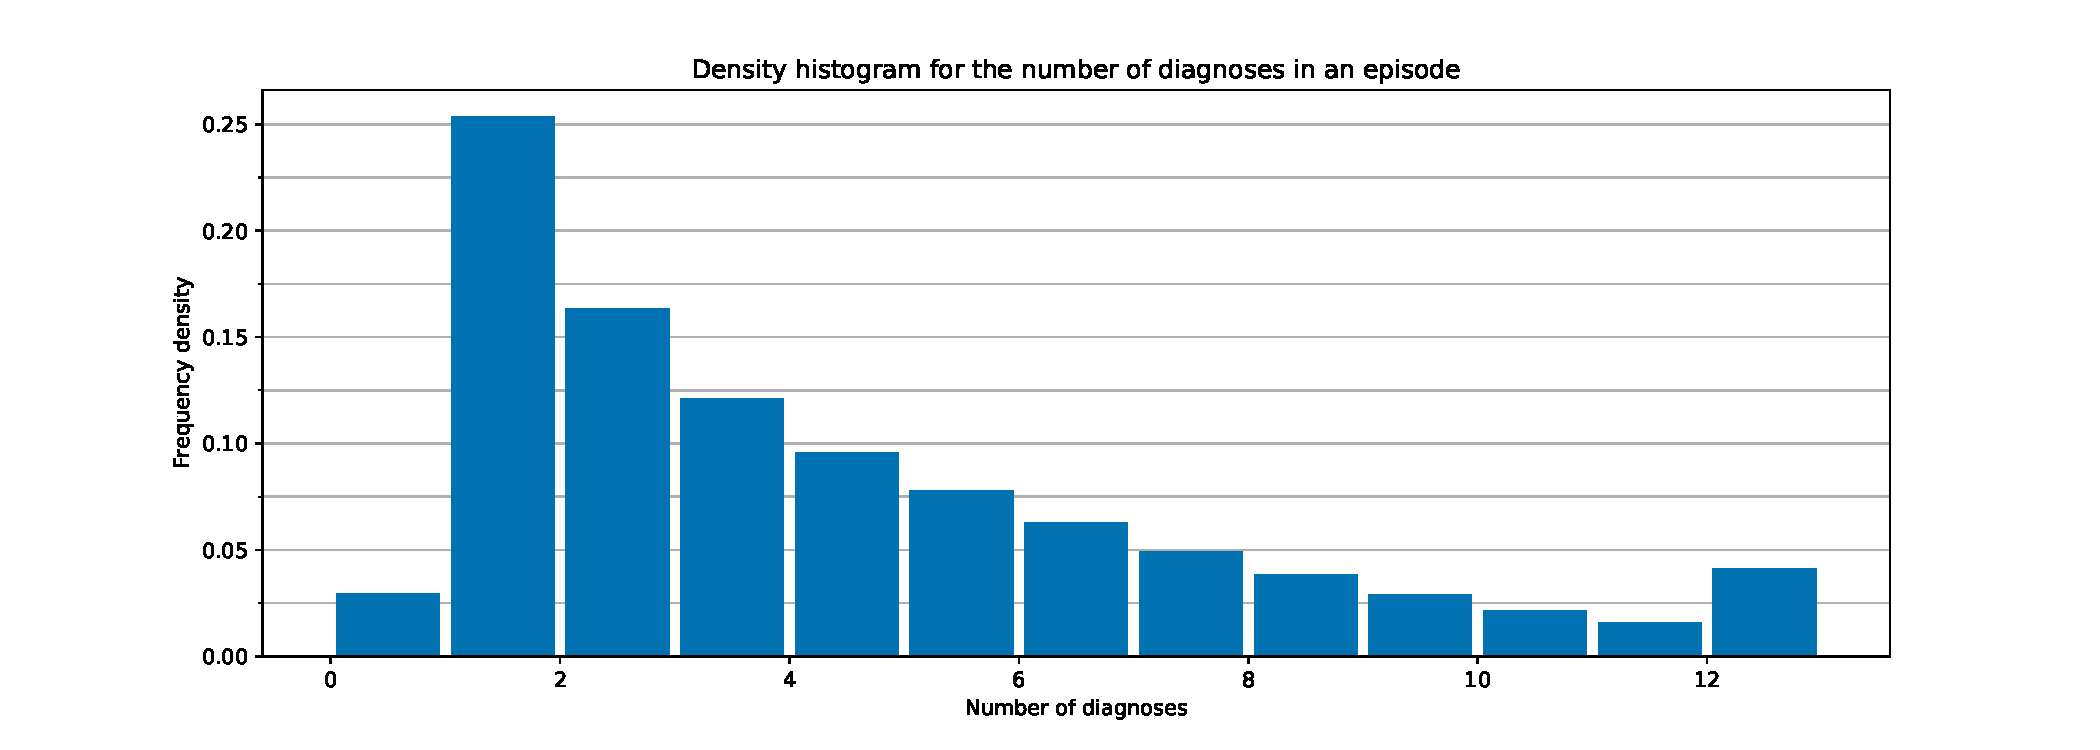
\includegraphics[width=\linewidth]{./img/diag_no_density_hist.pdf}
        \end{minipage}
    \end{figure}
\end{frame}

\begin{frame}
    \frametitle{Number of procedures}

    \begin{figure}
        \begin{minipage}{\linewidth}
            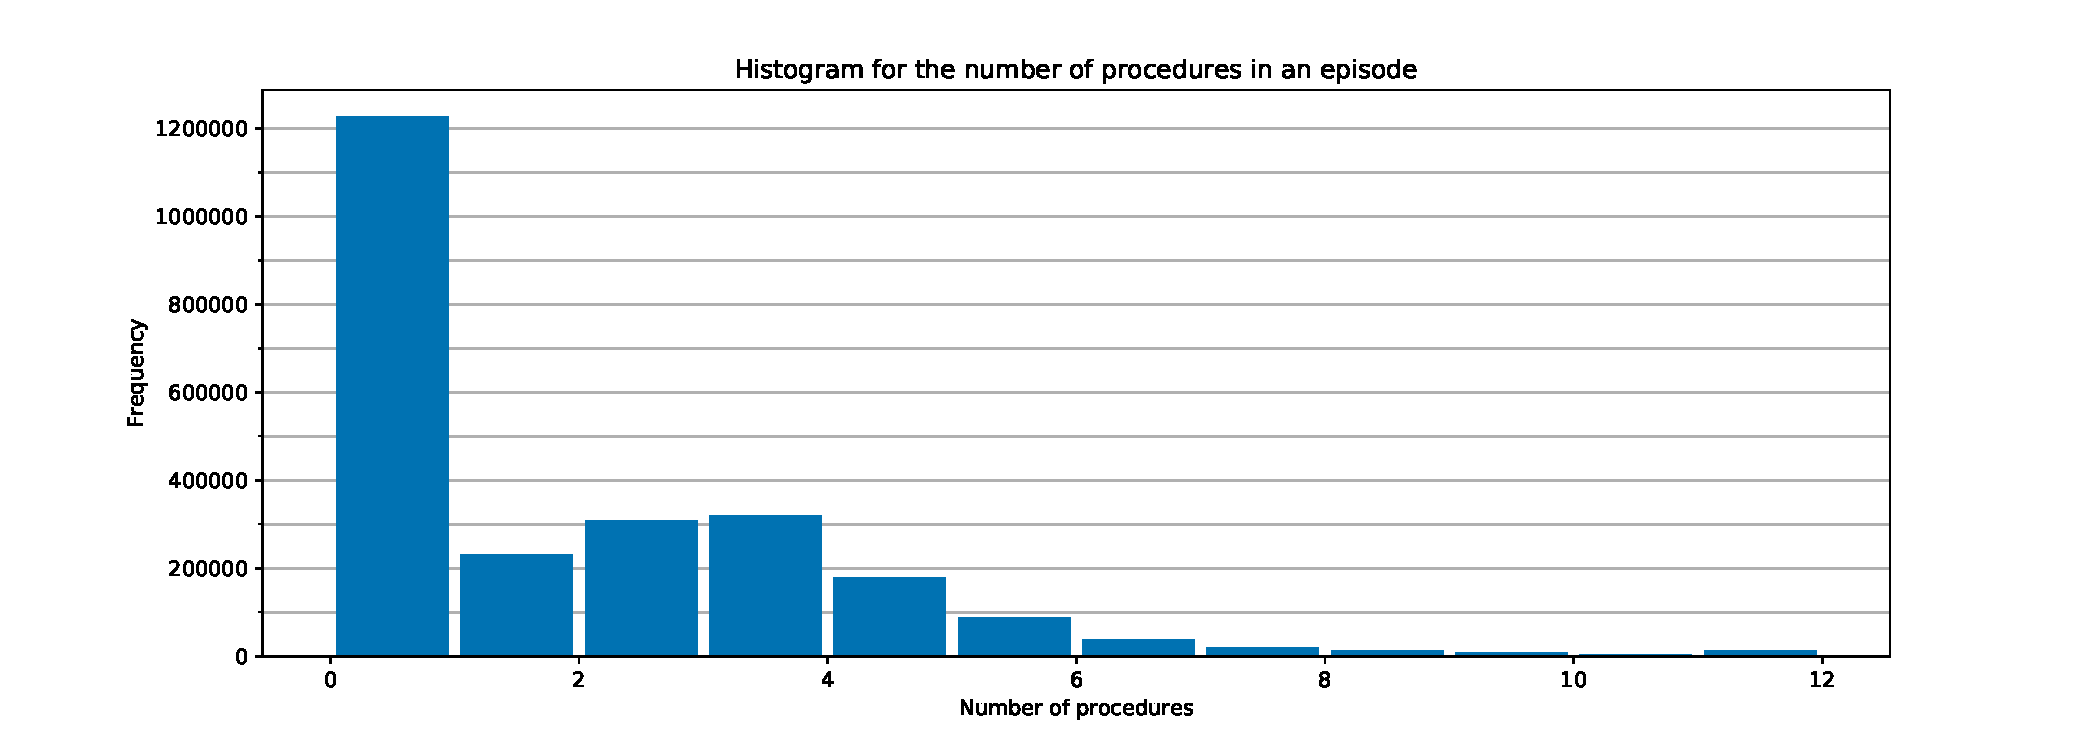
\includegraphics[width=\linewidth]{./img/proc_no_freq_hist.pdf}
        \end{minipage}
        \begin{minipage}{\linewidth}
            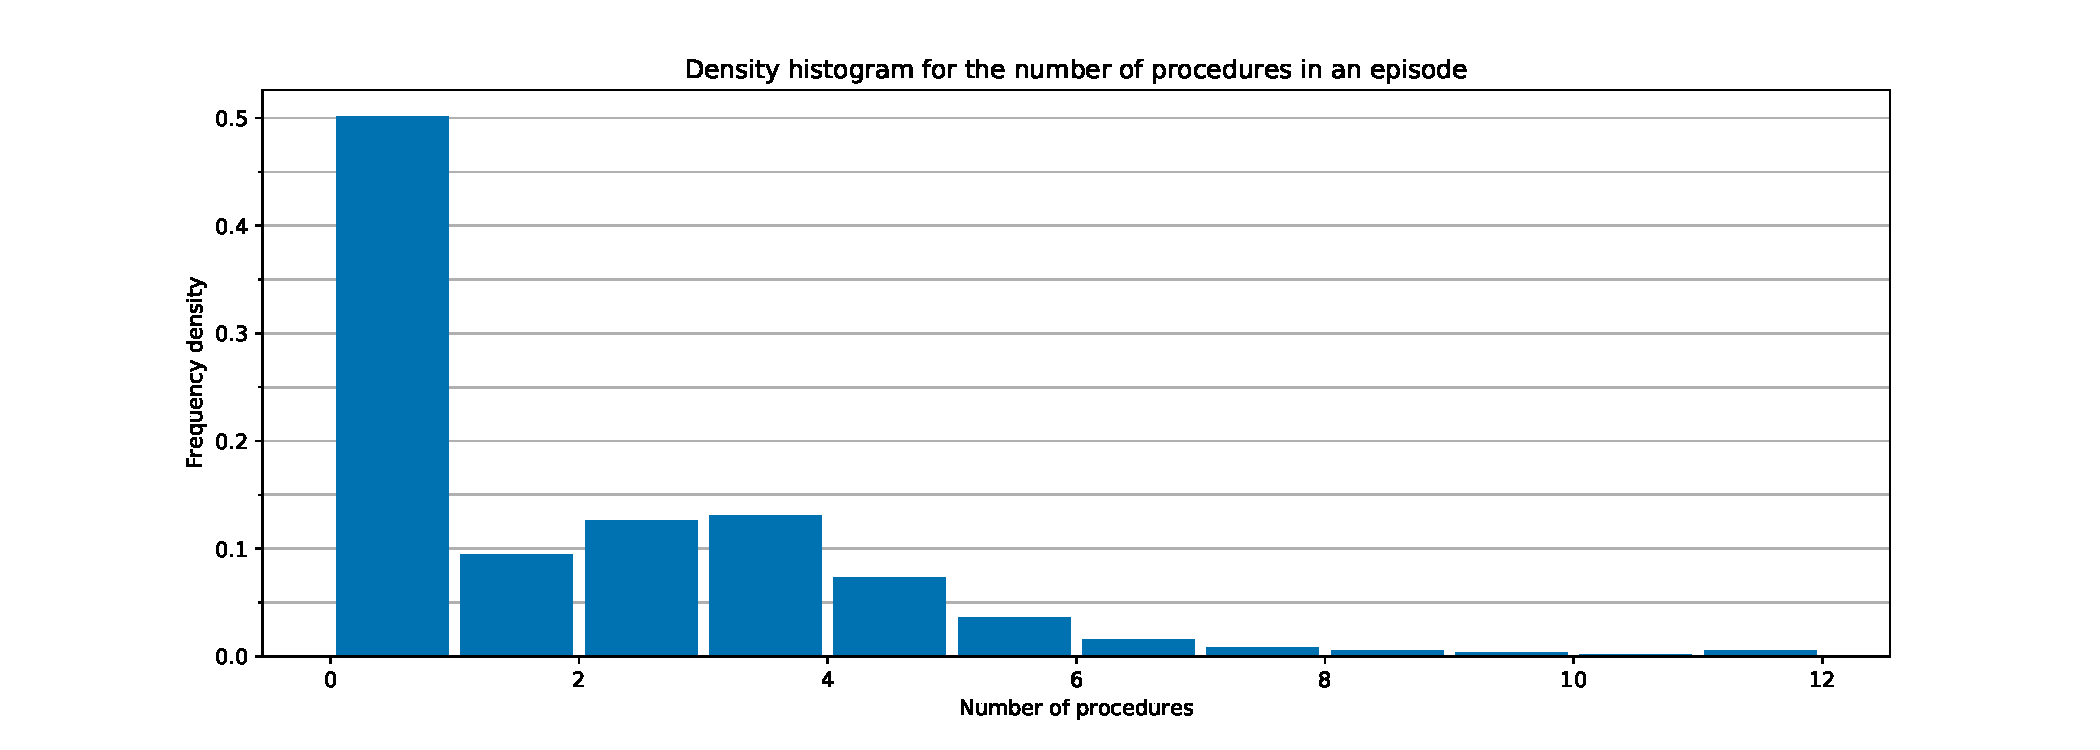
\includegraphics[width=\linewidth]{./img/proc_no_density_hist.pdf}
        \end{minipage}
    \end{figure}
\end{frame}

\begin{frame}
    \frametitle{Demographic analysis}

    As it stands, demographic information is not well-recorded in the data.

    \vspace{10pt}
    \begin{itemize}
        \pause%
        \item Gender is strictly binary and not recorded for all patients or
            episodes
        \pause%
        \item Limited geographic information is encoded in the GP practice code
            of the patient
    \end{itemize}
\end{frame}

\begin{frame}
    \frametitle{Demographic analysis}

    \begin{figure}
        \begin{minipage}{\linewidth}
            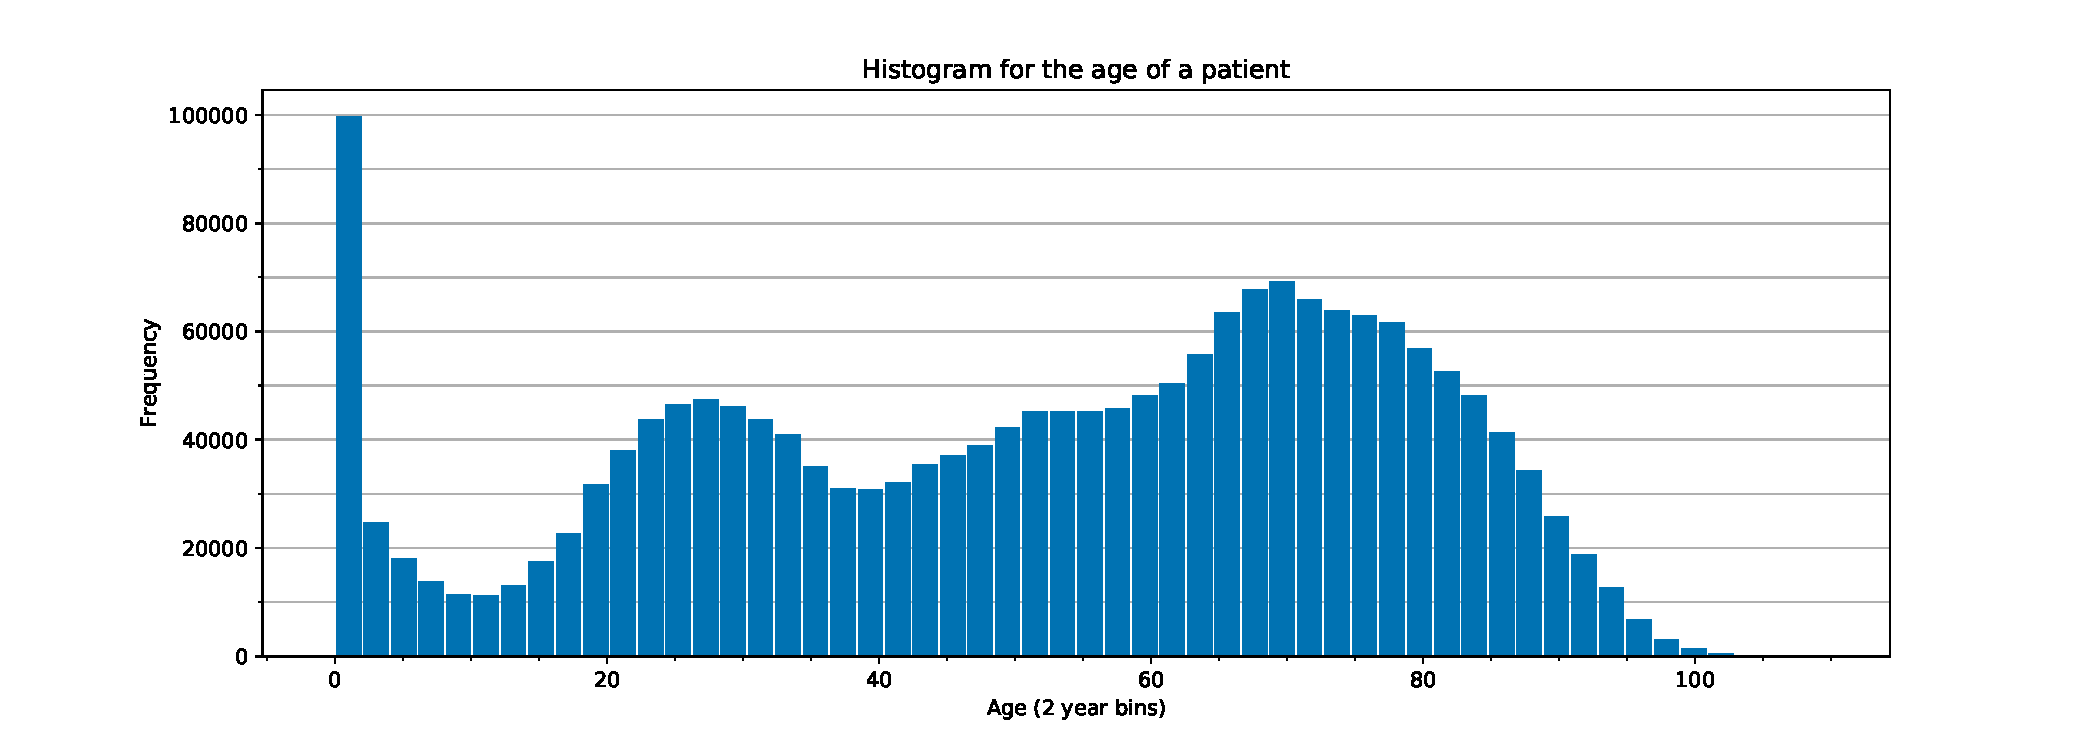
\includegraphics[width=\linewidth]{./img/age_freq_hist.pdf}
        \end{minipage}
        \begin{minipage}{\linewidth}
            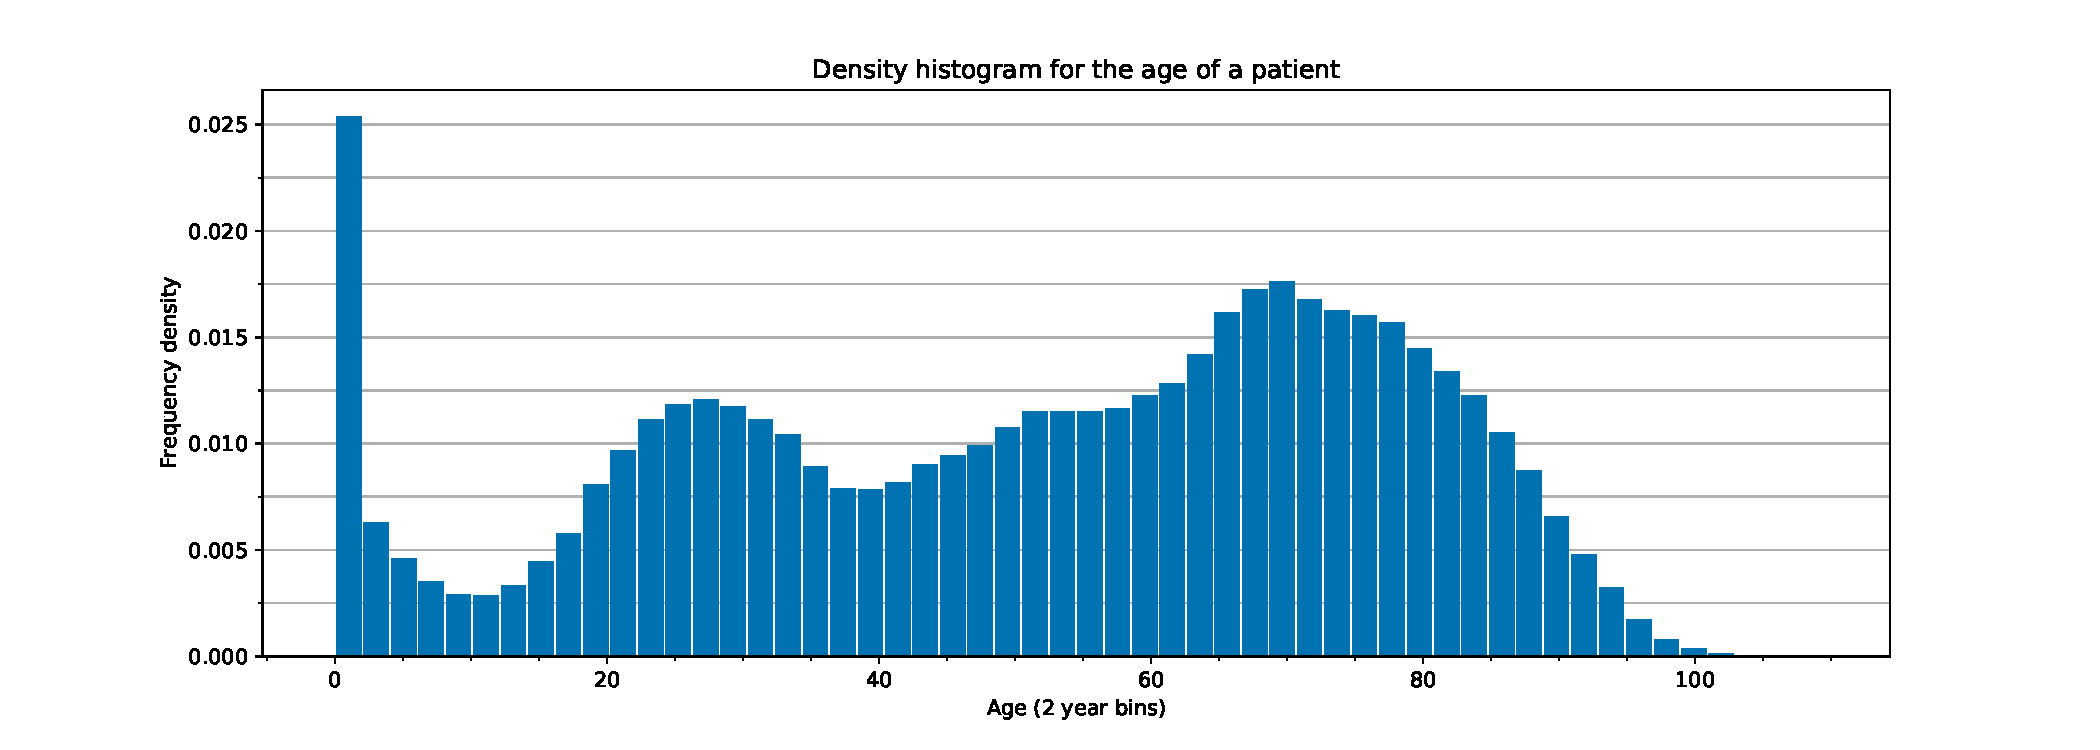
\includegraphics[width=\linewidth]{./img/age_density_hist.pdf}
        \end{minipage}
    \end{figure}
\end{frame}

\begin{frame}
    \frametitle{Correlation}

    \vspace{-15pt}
    \begin{figure}
        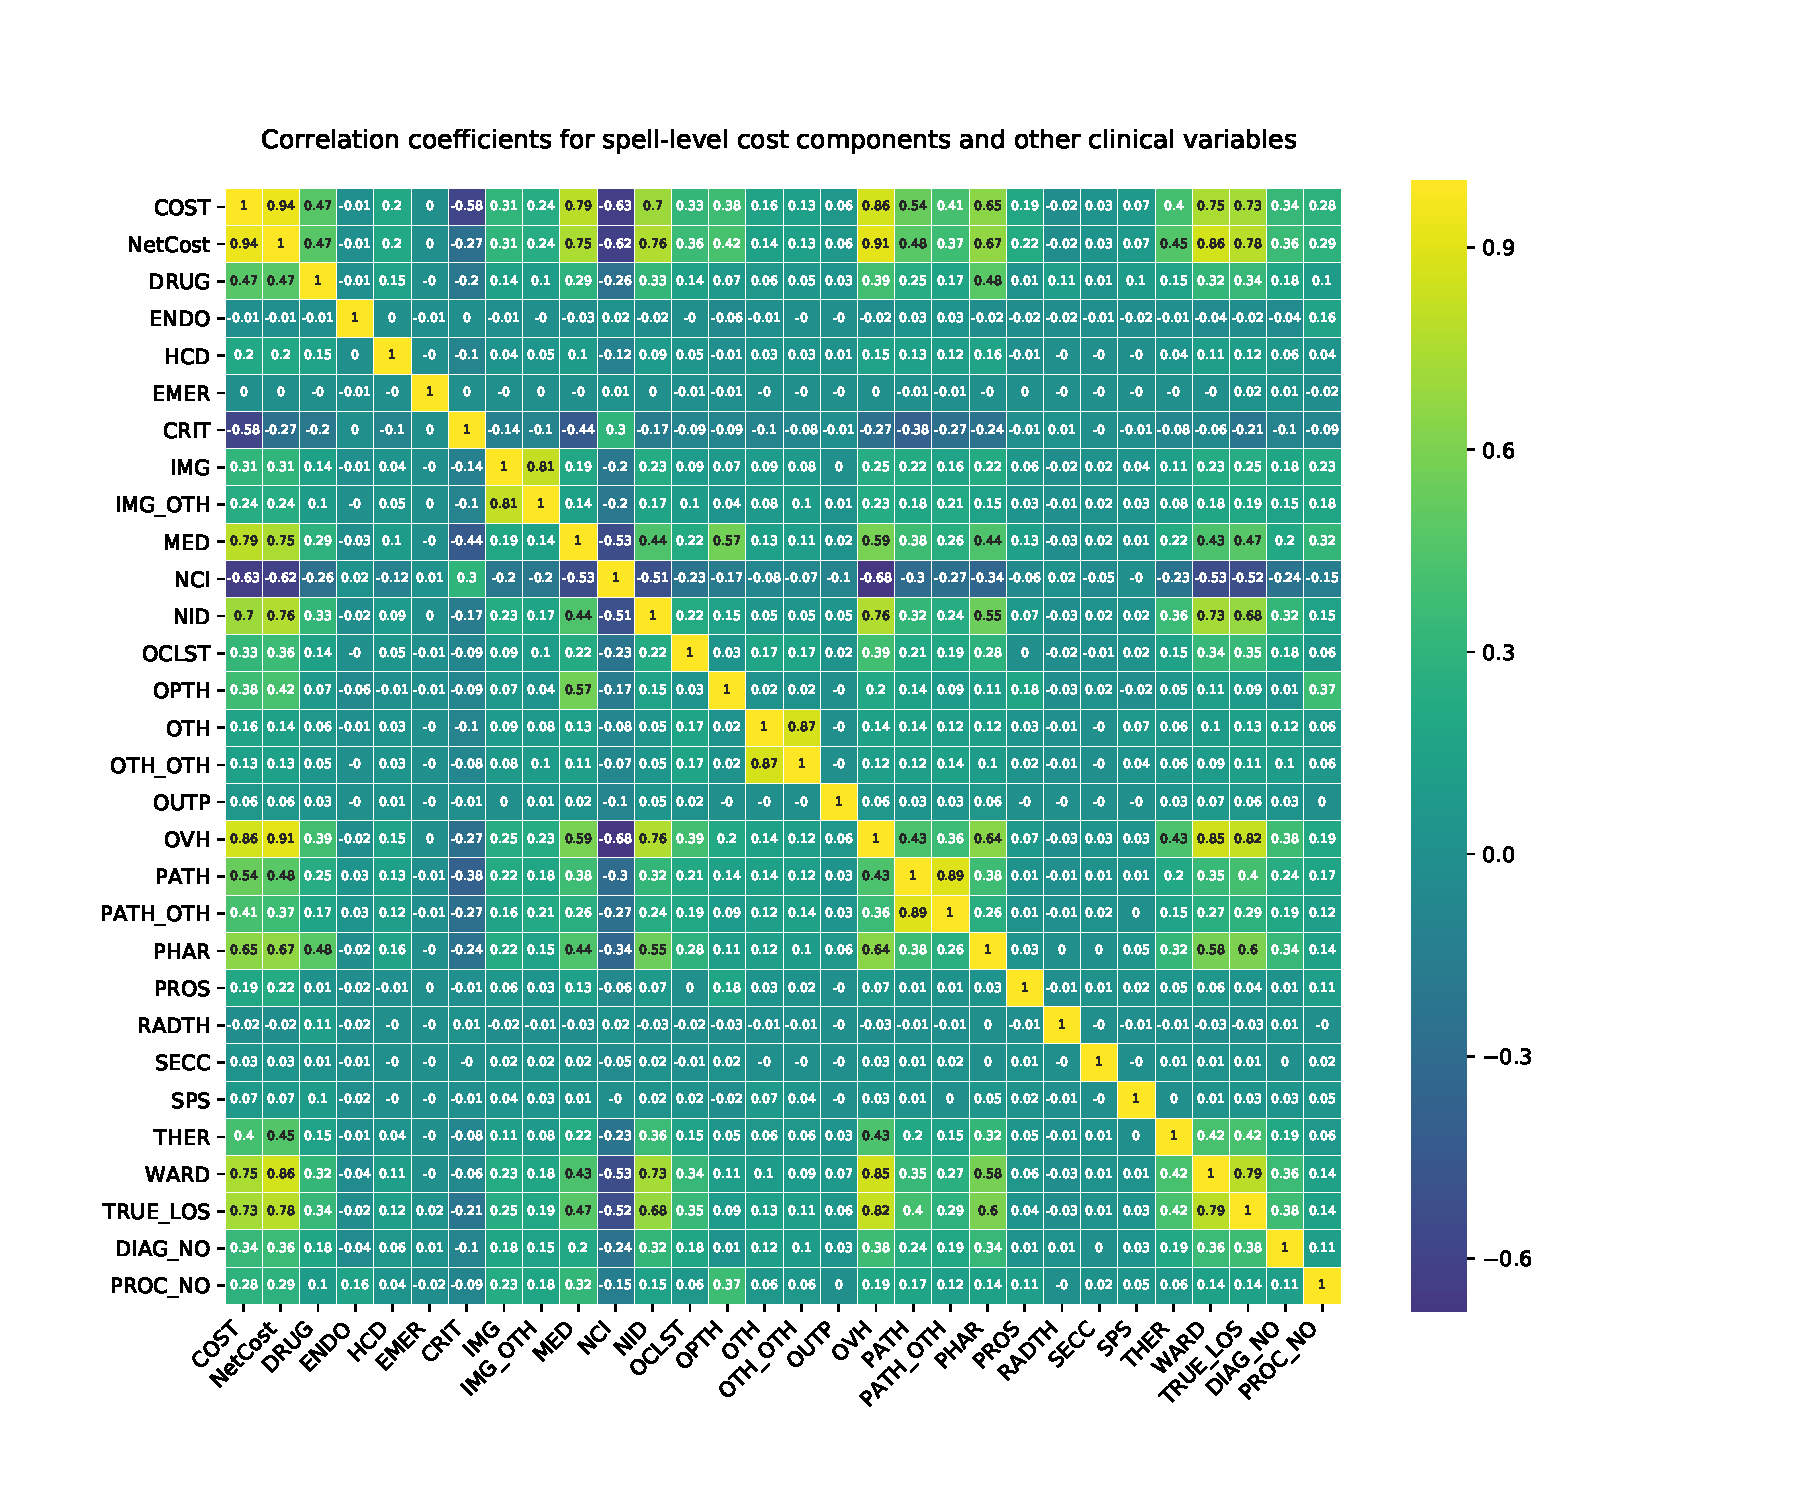
\includegraphics[width=\linewidth]{./img/corr_heatmap.pdf}
    \end{figure}
\end{frame}


\subsection{Measuring variation}

\begin{frame}
    \frametitle{Measuring variation}

    Variance is not scale invariant and did lead to misconceptions.

    \pause%
    \vspace{10pt}
    \begin{definition}
        Let \(\mu, \sigma^2\) denote the population mean and population variance
        of some population respectively. Then we define the
        \emph{coefficient~of~variation}, denoted by \(C_v\), to be:
        \[
            C_v = \frac{\sigma}{\mu}
        \]
    \end{definition}

    \pause%
    The coefficient of variation is scale invariant, and allows us to see the
    relative variation in each of our cost components.
\end{frame}

\begin{frame}
    \frametitle{Measuring variation}

    \begin{figure}
        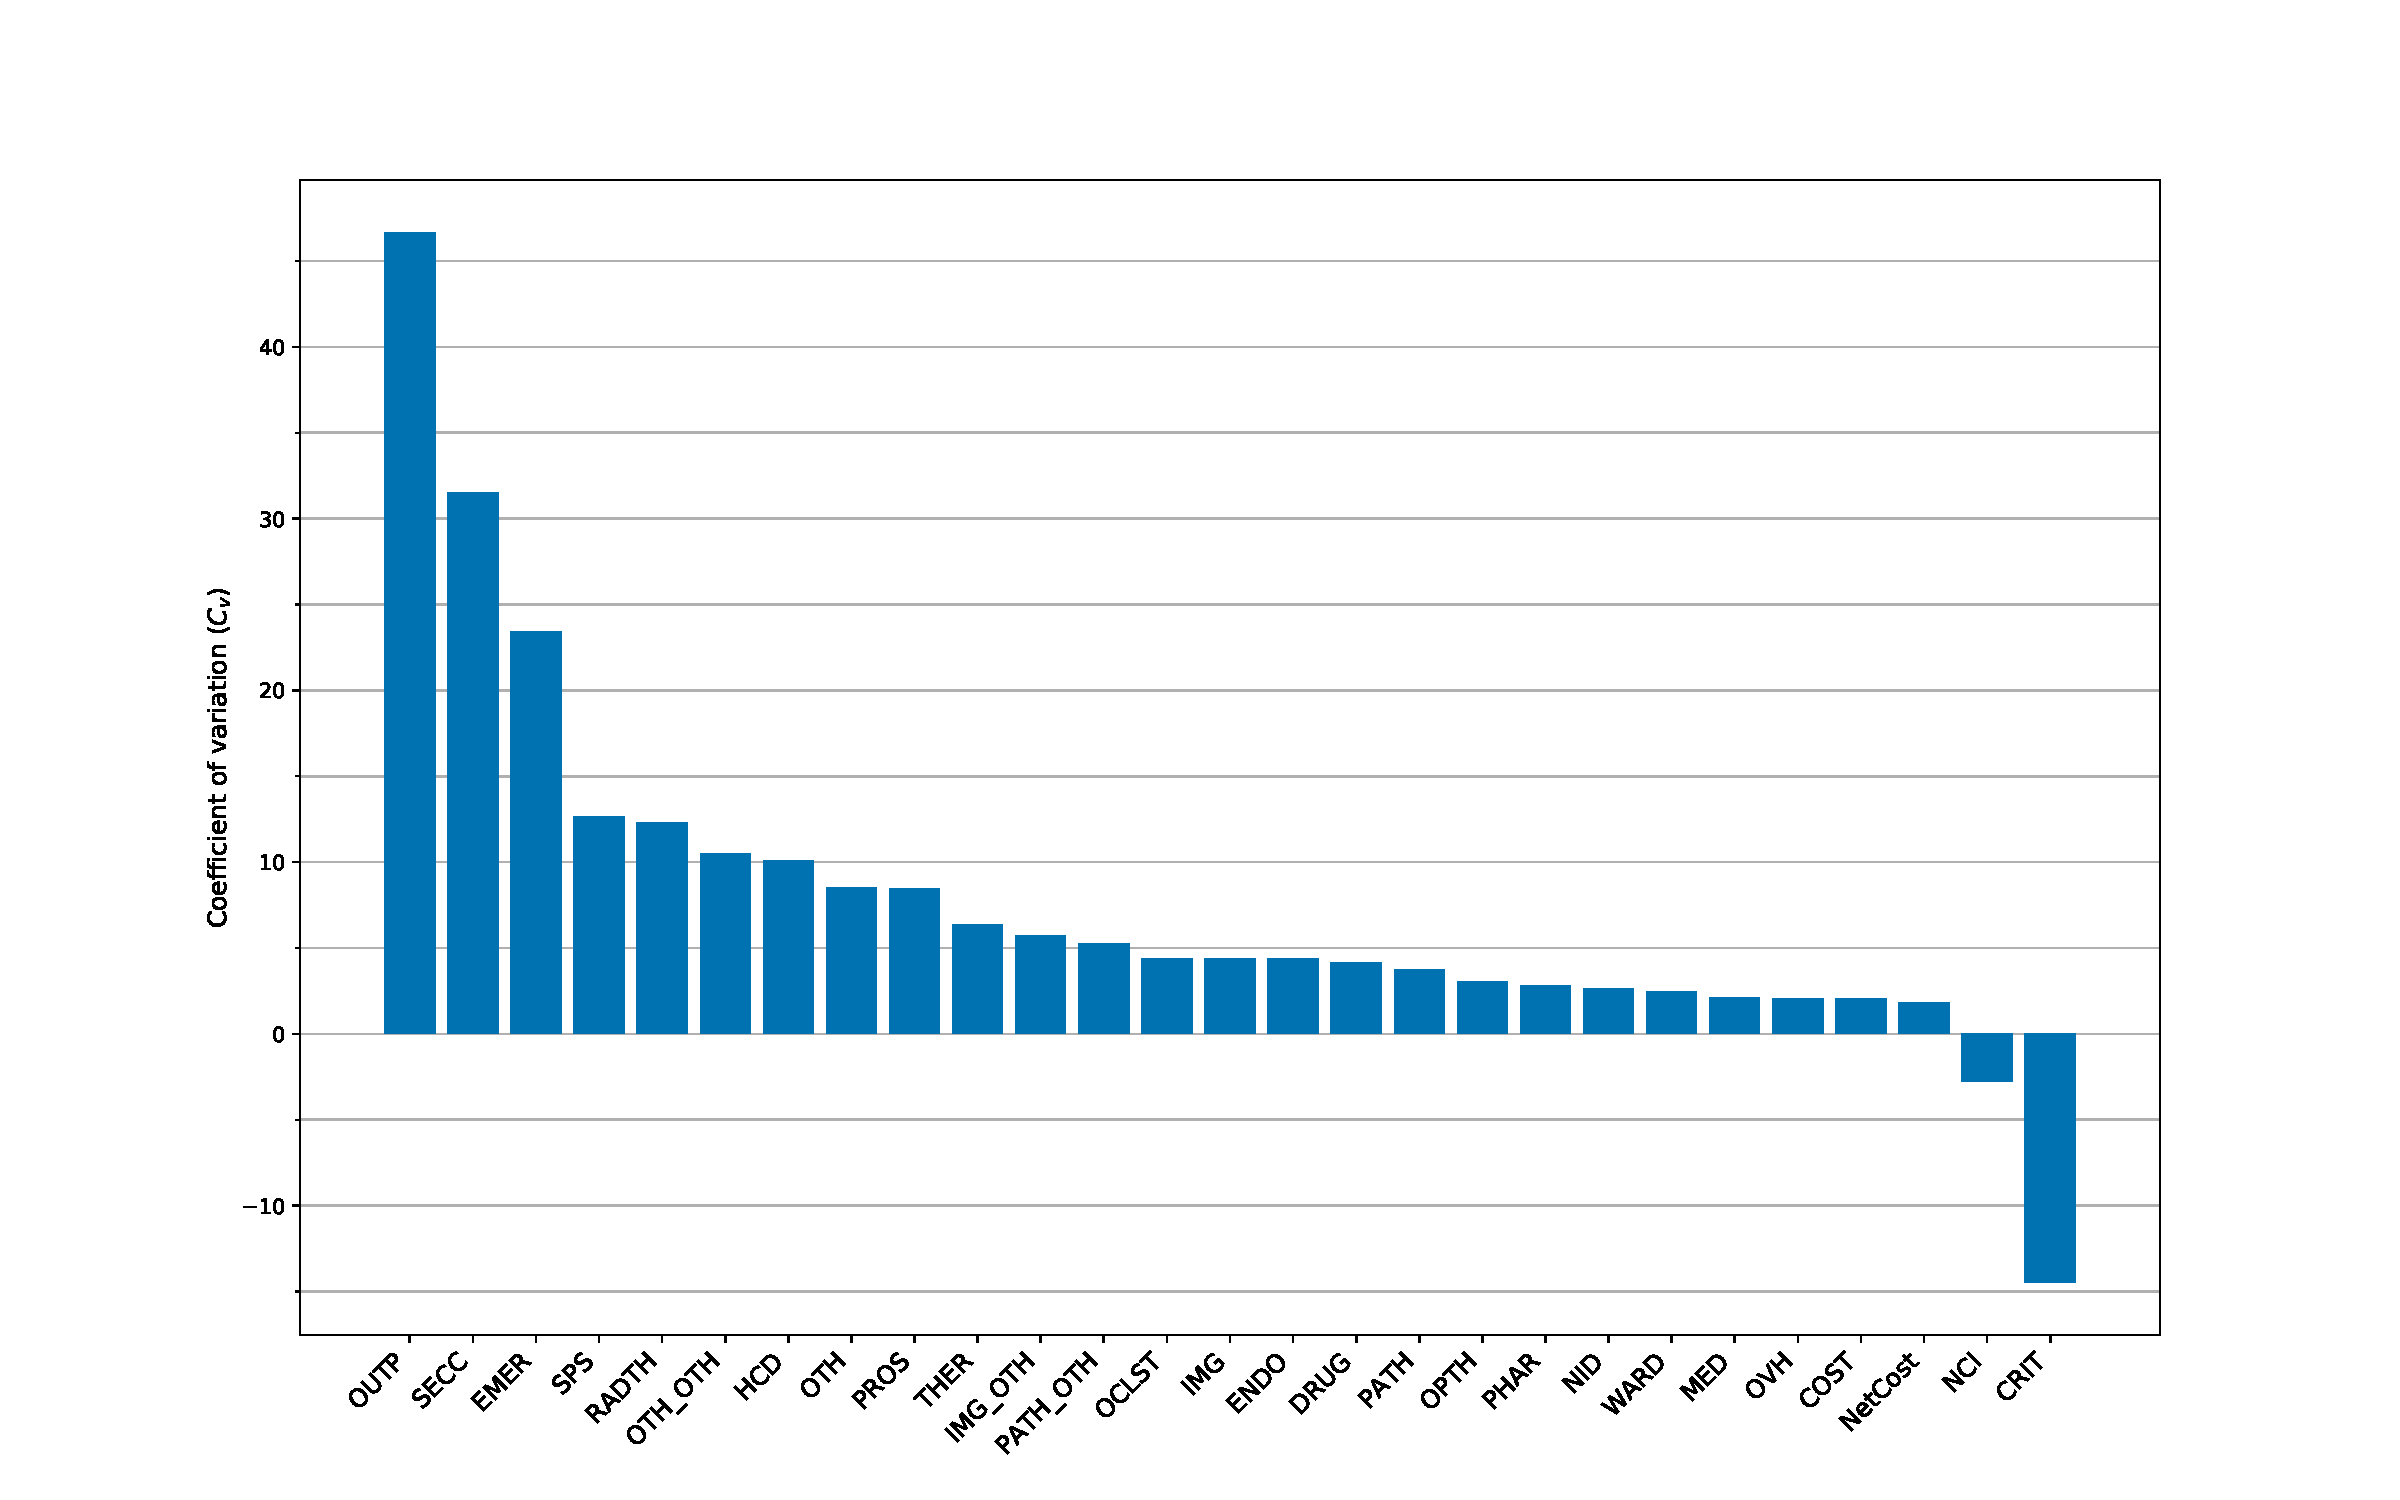
\includegraphics[width=\linewidth]{./img/coeff_variation.pdf}
    \end{figure}
\end{frame}

\begin{frame}
    \frametitle{Are these actually important?}

    Despite the relative variation of our cost components being whatever value,
    does it matter to the actual cost?

    \vspace{10pt}
    Let us investigate their contribution to the final cost.
\end{frame}

\begin{frame}
    \frametitle{Cost component contribution}

    \begin{figure}
        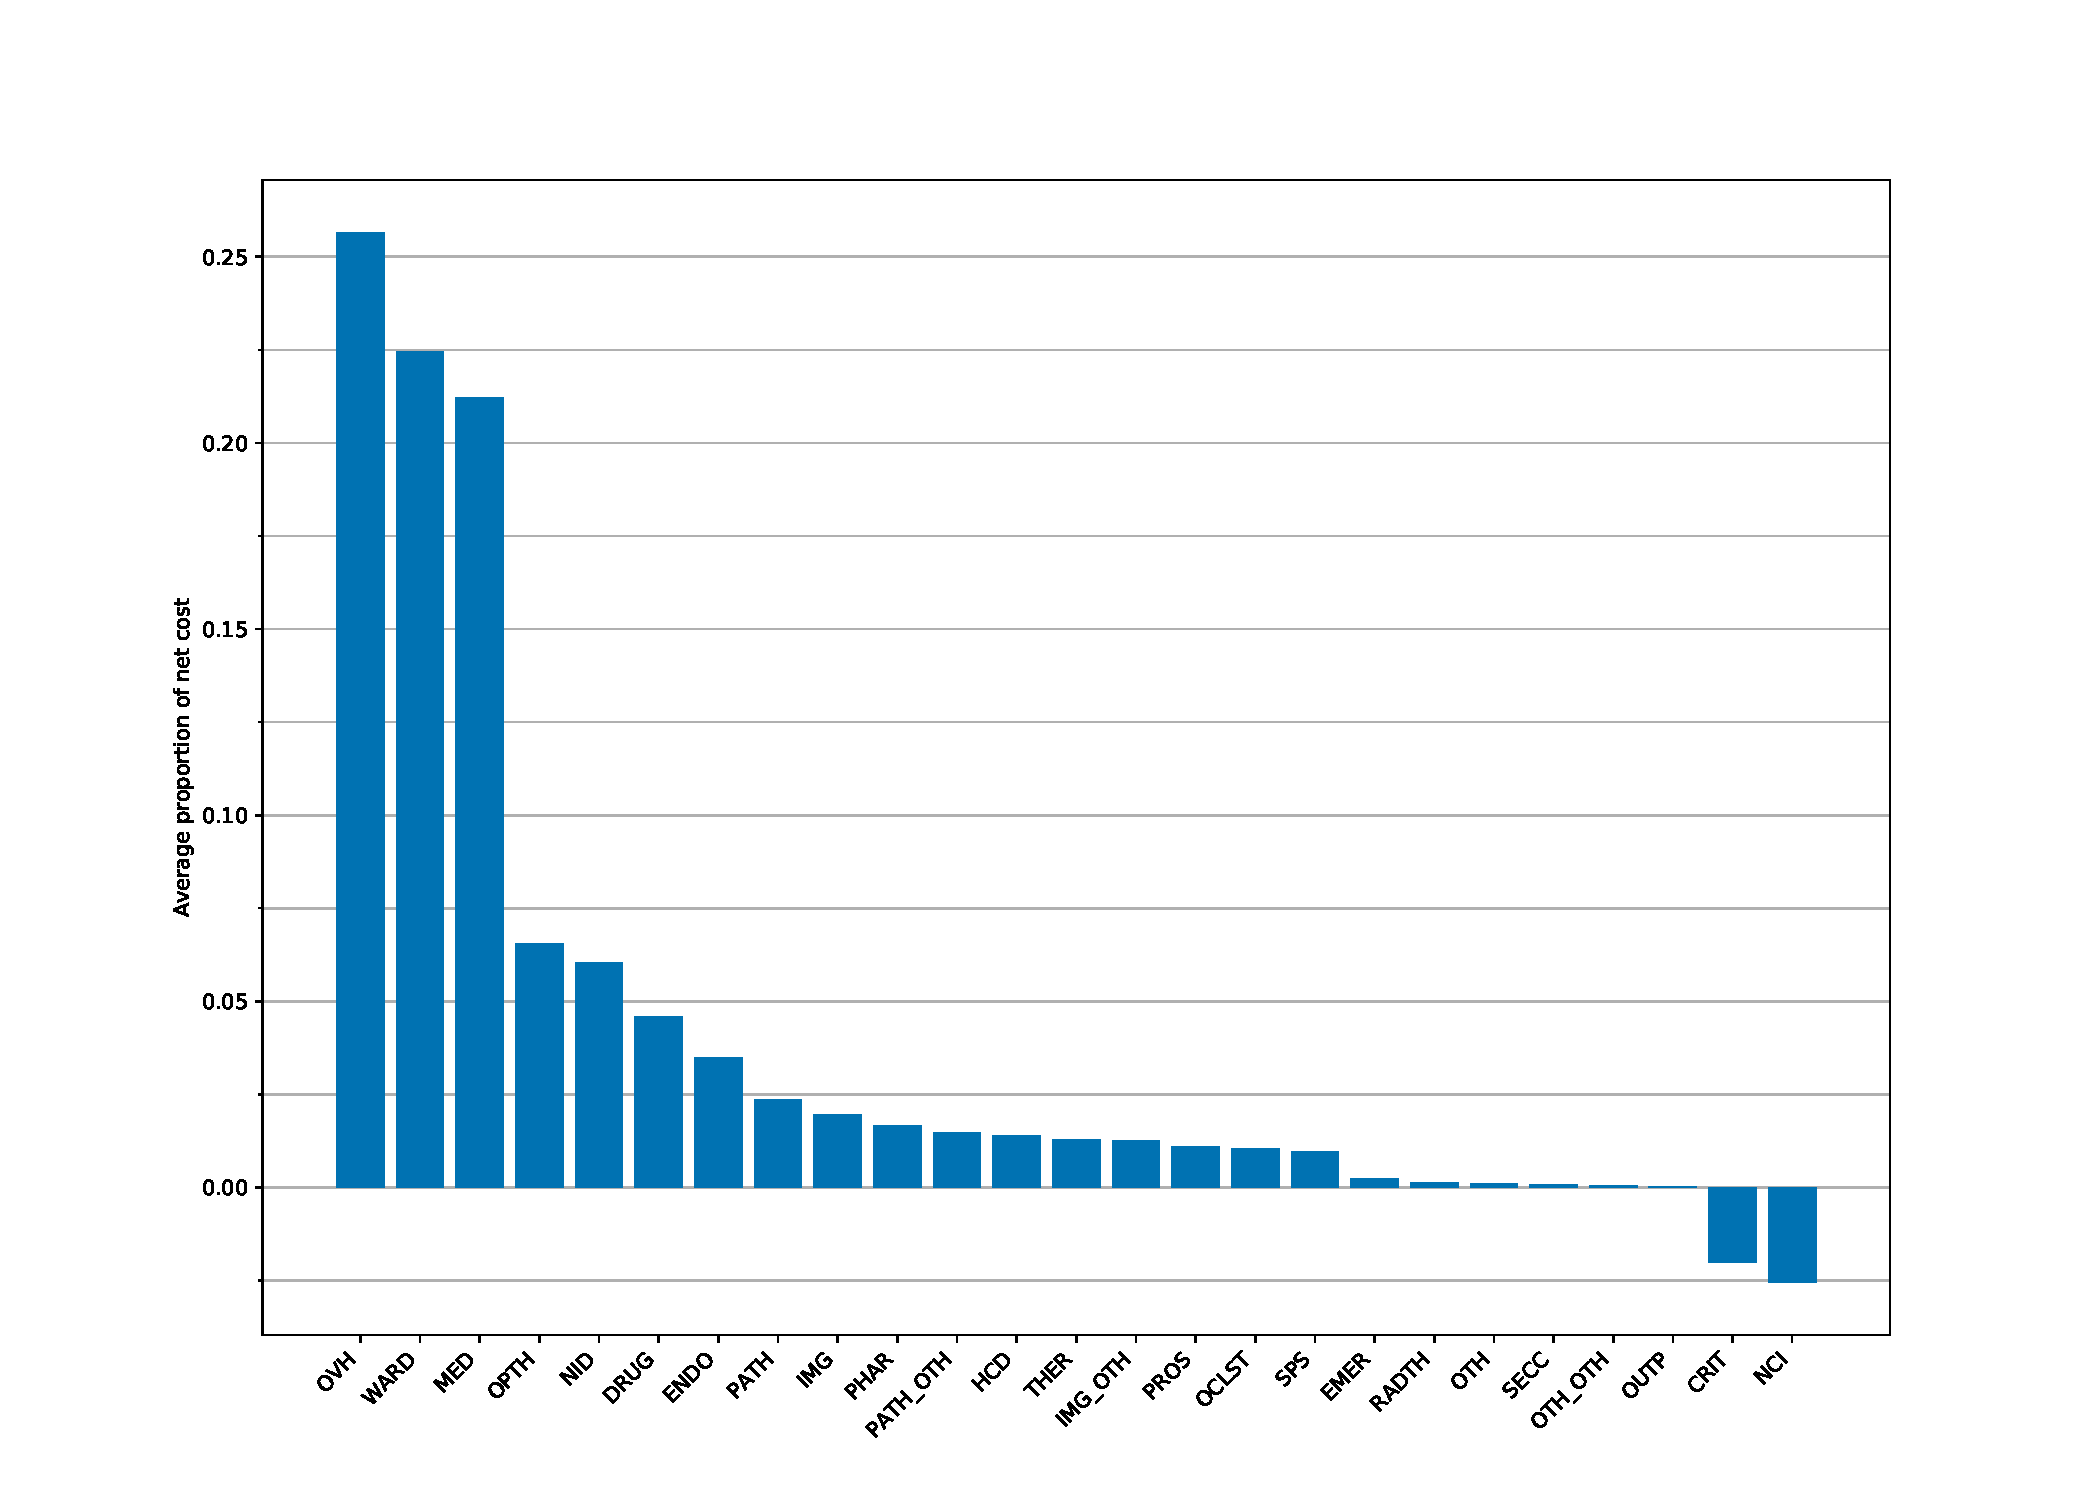
\includegraphics[width=\linewidth]{./img/cost_contribution.pdf}
    \end{figure}
\end{frame}


\section{Slice analysis}

\subsection{General methodology}

\begin{frame}
    \frametitle{General methods for slice analysis}

    Given some slice of the data, we want to:
    \begin{itemize}
        \item Examine cost variations and general surface-level statistics
        \item Determine components and variable relationships of interest
        \item Consider the relative `cost' of the patients in this slice
        \item Contrast this against its complement and the general dataset
    \end{itemize}
\end{frame}

\subsection{Diabetic patient analysis}

\begin{frame}
    \frametitle{Diabetic patient analysis}

    This is a known area of interest to the health board.

    \vspace{10pt}
    Diabetic patients make up 10.8\% of all the episodes in the dataset, and
    roughly 8.7\% of the unique patients in the dataset.

    \vspace{10pt}
    Here we consider patients to be `diabetic' if they have diabetes flagged as
    either a primary or secondary condition in their episode.
\end{frame}

\begin{frame}
    \frametitle{Number of spells}

    \begin{figure}
        \begin{minipage}{\linewidth}
            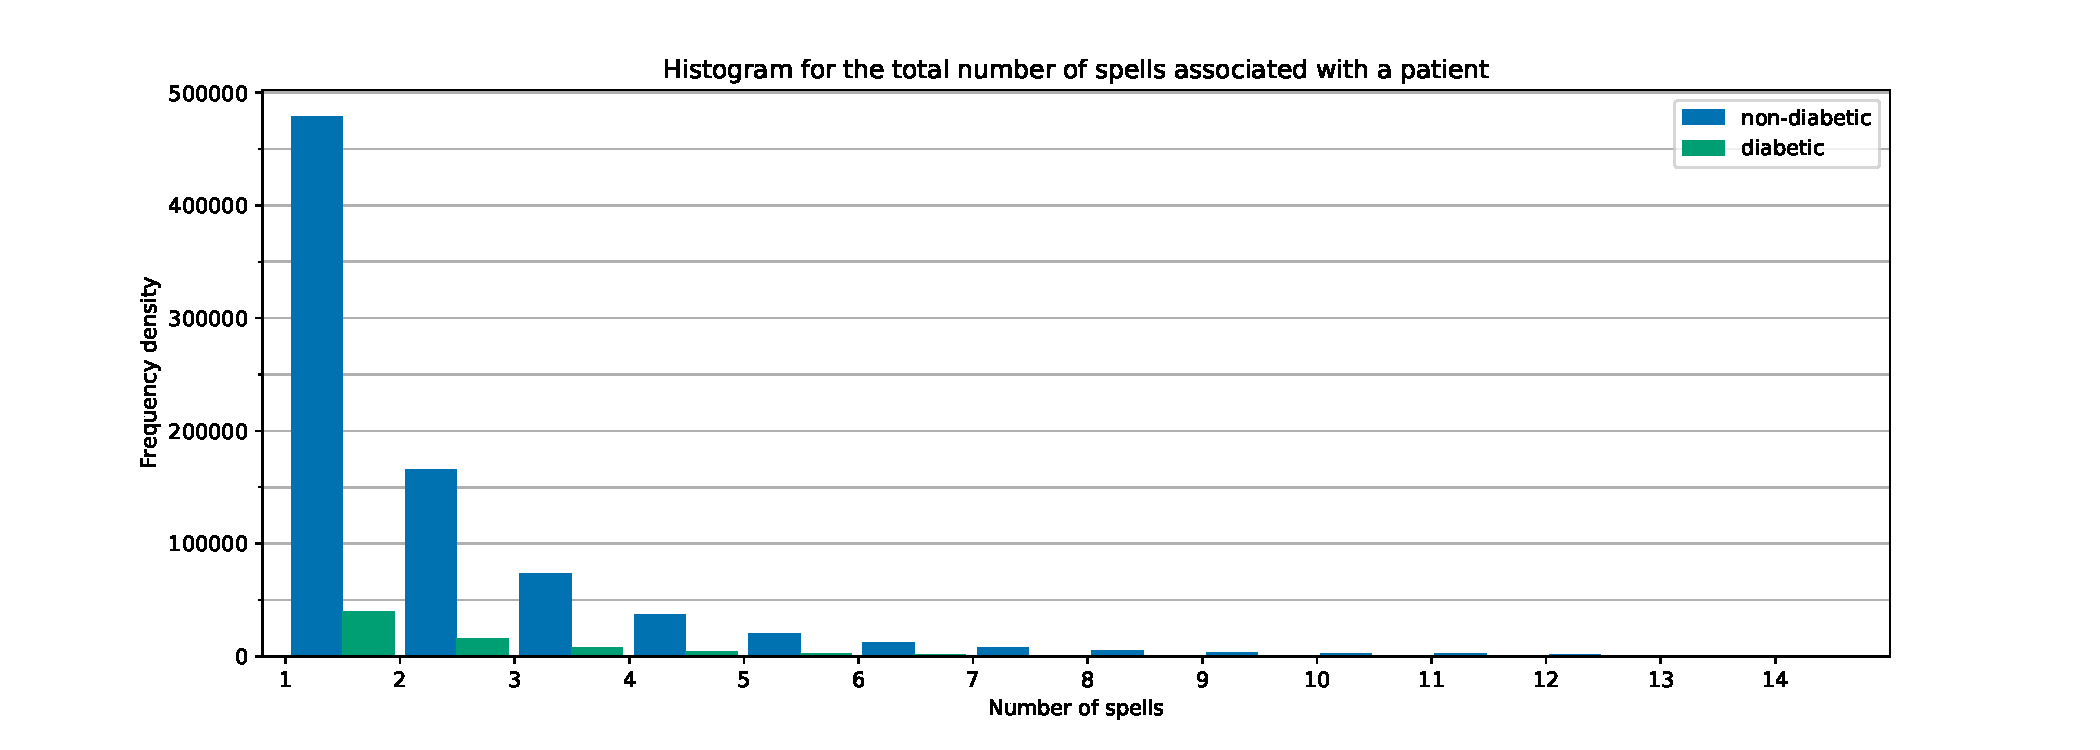
\includegraphics[width=\linewidth]
                {./img/diabetic_no_spells_freq_hist.pdf}
        \end{minipage}
        \begin{minipage}{\linewidth}
            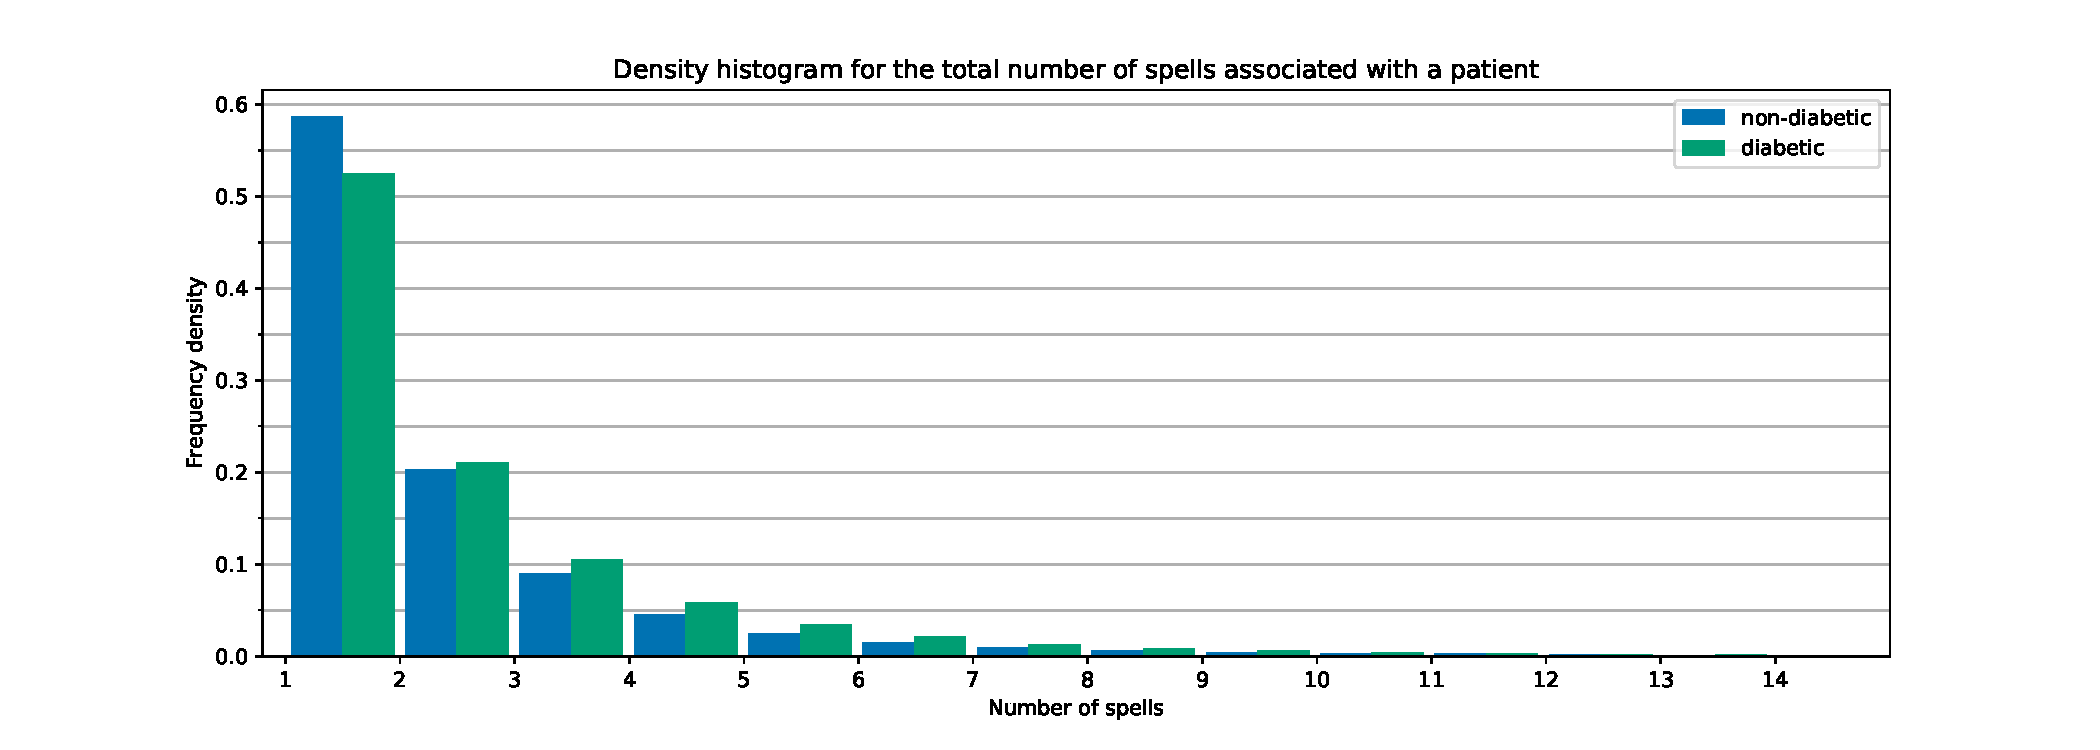
\includegraphics[width=\linewidth]
                {./img/diabetic_no_spells_density_hist.pdf}
        \end{minipage}
    \end{figure}
\end{frame}

\begin{frame}
    \frametitle{Length of stay}

    \begin{figure}
        \begin{minipage}{\linewidth}
            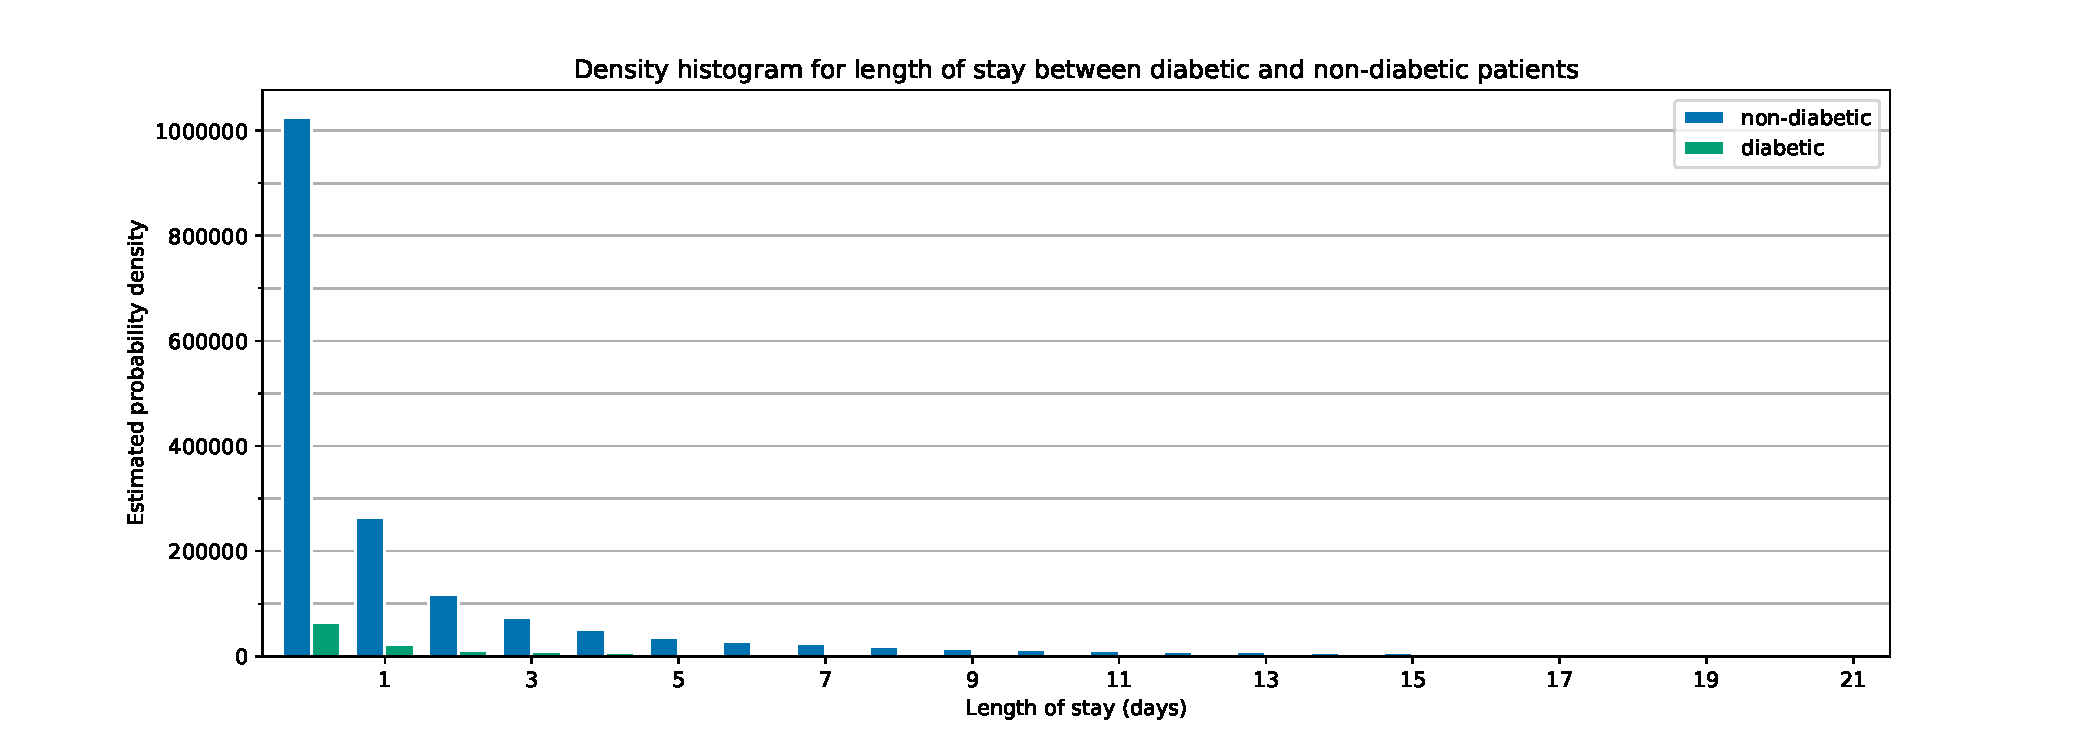
\includegraphics[width=\linewidth]{./img/diabetic_LOS_freq_hist.pdf}
        \end{minipage}
        \begin{minipage}{\linewidth}
            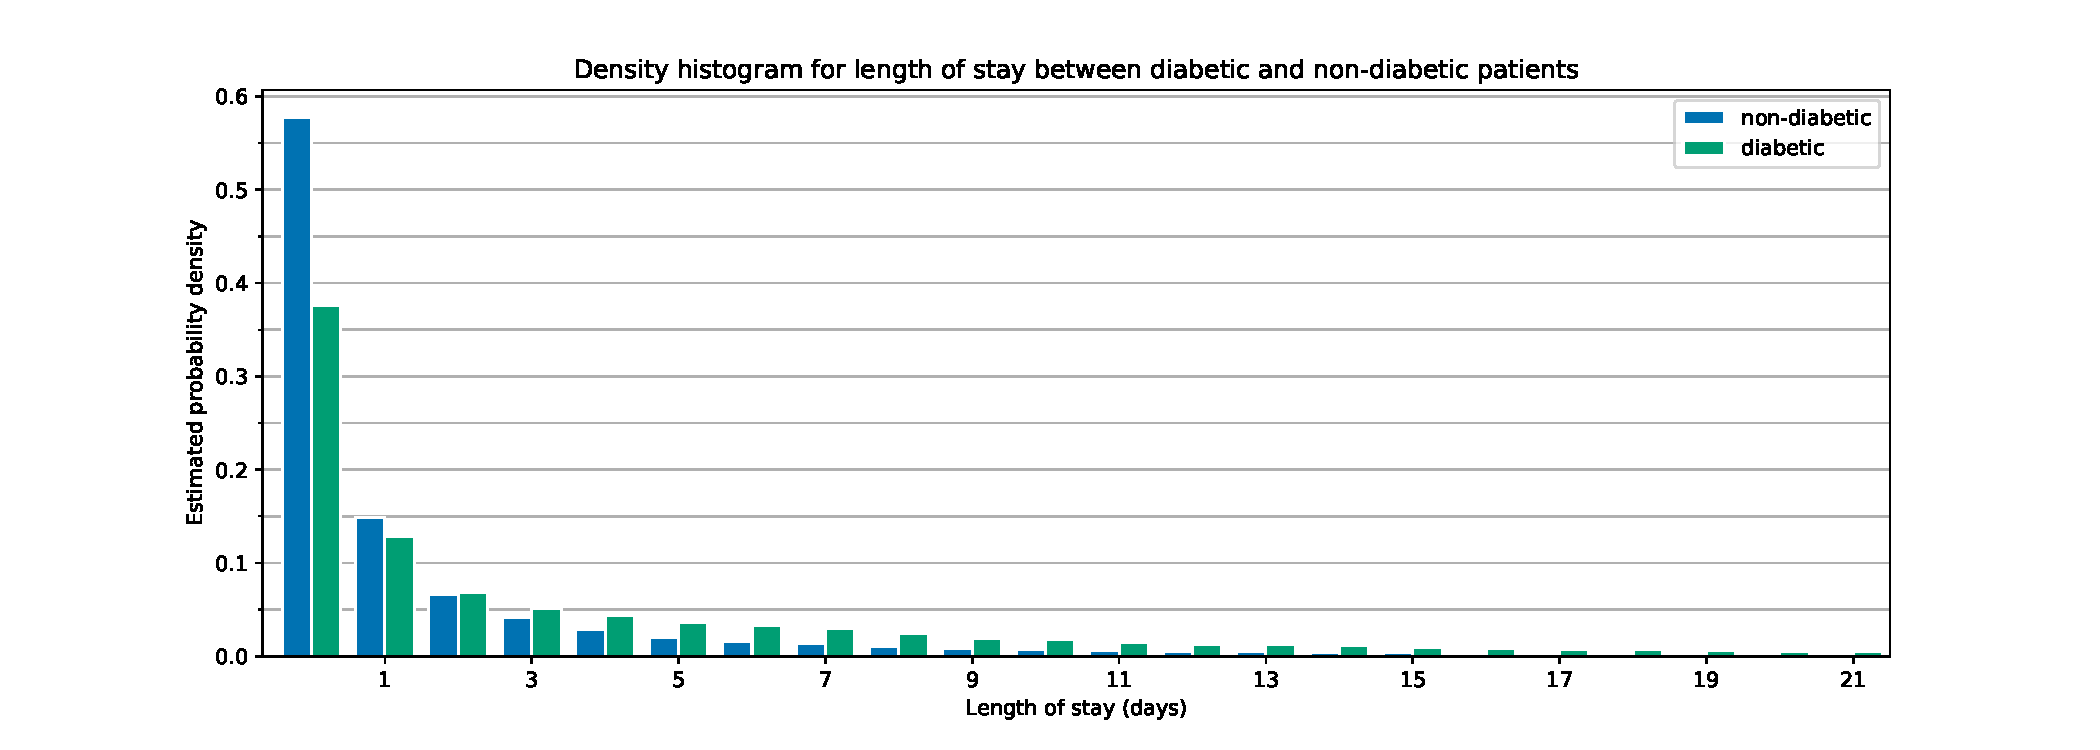
\includegraphics[width=\linewidth]
                {./img/diabetic_LOS_density_hist.pdf}
        \end{minipage}
    \end{figure}
\end{frame}

\begin{frame}
    \frametitle{Net cost}

    \begin{figure}
        \includegraphics[width=\linewidth]{./img/diabetic_netcost_kde.pdf}
    \end{figure}
\end{frame}

\begin{frame}
    \frametitle{Number of diagnoses}
   
    \begin{figure}
        \begin{minipage}{\linewidth}
            \includegraphics[width=\linewidth]
                {./img/diabetic_diag_no_freq_hist.pdf}
        \end{minipage}
        \begin{minipage}{\linewidth}
            \includegraphics[width=\linewidth]
                {./img/diabetic_diag_no_density_hist.pdf}
        \end{minipage}
    \end{figure}
\end{frame}

\begin{frame}
    \frametitle{Number of procedures}

    \begin{figure}
        \begin{minipage}{\linewidth}
            \includegraphics[width=\linewidth]
                {./img/diabetic_proc_no_freq_hist.pdf}
        \end{minipage}
        \begin{minipage}{\linewidth}
            \includegraphics[width=\linewidth]
                {./img/diabetic_proc_no_density_hist.pdf}
        \end{minipage}
    \end{figure}
\end{frame}

\begin{frame}
    \frametitle{Demographic analysis}

    \begin{figure}
        \begin{minipage}{\linewidth}
            \includegraphics[width=\linewidth]{./img/diabetic_age_freq_hist.pdf}
        \end{minipage}
        \begin{minipage}{\linewidth}
            \includegraphics[width=\linewidth]
                {./img/diabetic_age_density_hist.pdf}
        \end{minipage}
    \end{figure}
\end{frame}

\begin{frame}
    \frametitle{Cost variation}

    \begin{figure}
        \includegraphics[width=\linewidth]{./img/diabetic_coeff_variation.pdf}
    \end{figure}
\end{frame}

\begin{frame}
    \frametitle{Cost component contribution}

    \begin{figure}
        \includegraphics[width=\linewidth]{./img/diabetic_cost_contribution.pdf}
    \end{figure}
\end{frame}

\begin{frame}
    \frametitle{Correlation}

    \vspace{-15pt}
    \begin{figure}
        \includegraphics[width=\linewidth]{./img/diabetic_corr_heatmap.pdf}
    \end{figure}
\end{frame}

\begin{frame}
    \frametitle{Correlation (differences)}

    \vspace{-15pt}
    \begin{figure}
        \includegraphics[width=\linewidth]{./img/differences_corr_heatmap.pdf}
    \end{figure}
\end{frame}

\begin{frame}
    \frametitle{Diabetic patient analysis}

    We will focus our definition of system `cost' on three measures:

    \pause%
    \begin{itemize}
        \item Proportion of total daily admissions
        \item Average length of stay given admission date
        \item Proportion of net costs spent given admission date
    \end{itemize}

    \pause%
    \vspace{10pt}
    These are indicators of resources used and resources necessary.

    \vspace{10pt}
    This grouping by admission date will lead to a degree of misrepresentation
    in our plots.

    \vspace{10pt}
    Allows us to investigate patterns developing over time.
\end{frame}

\begin{frame}
    \frametitle{Resource consumption}

    \begin{figure}
        \includegraphics[width=\linewidth]{./img/diabetic_admissions.pdf}
    \end{figure}
\end{frame}

\begin{frame}
    \frametitle{Resource consumption}

    \begin{figure}
        \includegraphics[width=\linewidth]{./img/diabetic_LOS_time.pdf}
    \end{figure}
\end{frame}

\begin{frame}
    \frametitle{Resource consumption}

    \begin{figure}
        \includegraphics[width=\linewidth]
            {./img/diabetic_netcost_proportions.pdf}
    \end{figure}
\end{frame}

\begin{frame}
    \frametitle{Conclusions}

    \begin{itemize}
        \item Relative resource consumption by diabetic patients is consistent
        \item Cost components are less variant than \-- and are comparable in
            their distribution to \-- non-diabetic patients
    \end{itemize}
\end{frame}

\section{Moving forward}

\begin{frame}
    \frametitle{Moving forward}
    \begin{itemize}
        \pause%
        \item Resource consumption metric
        \pause%
        \item Perform clustering analysis to find inherent slices in the data
        \pause%
        \item Incorporate external data
        \begin{itemize}
            \item Decode GP practice codes for GeoPandas
            \item Socio-economic analysis based on deprivation and geography
            \item Temperature-based analysis
        \end{itemize}
        \pause%
        \item Severity and comorbidity analysis
        \begin{itemize}
            \item Average severity of secondary conditions given some primary
                condition
            \item Using the comorbidity index as a class label in some
                predictive analysis
        \end{itemize}
    \end{itemize}
\end{frame}

\end{document}

\documentclass{beamer}

\usepackage{graphicx}

\title{An exploratory analysis of patient episode data}
\author{Henry Wilde}
\institute{Cardiff University School of Mathematics}

\usetheme{Hannover}
\usecolortheme{seahorse}
\begin{document}

\begin{frame}
\titlepage%
\end{frame}

\begin{frame}
\frametitle{Outline}
\tableofcontents
\end{frame}

\section{Motivation}

\begin{frame}
\frametitle{Motivation}

\begin{itemize}
    \item Observe and understand cost variation
    \item Identify important slices in the data
    \item Develop methods for examining slices of the data
    \item Analyse their impact on costs and resource consumption
\end{itemize}
\end{frame}

\section{Getting to know the data}

\subsection{Structure and origin}
\begin{frame}
    \frametitle{Structure and origin}

    \pause%
    All data is provided by the Cwm Taf University Health Board.
    \vspace{10pt}

    \pause%
    We have:
    \begin{itemize}
        \item 2,447,299 patient episodes
        \item 1,946,545 patient spells
        \item 865,421 individual patients
    \end{itemize}
    \vspace{10pt}

    \pause%
    Each row is made up of roughly 250 attributes, including:
    \begin{itemize}
        \pause%
        \item personal identifiers and demographic information
        \pause%
        \item condition and treatment indicators (HRG, OPCS4, ICD10)
        \pause%
        \item other clinical references
        \pause%
        \item cost components
    \end{itemize}
\end{frame}

\subsection{Summative analysis}
\begin{frame}
    \frametitle{Summative analysis}

    \begin{itemize}
        \pause%
        \item Our data is skewed towards low-cost, short-stay episodes
        \pause%
        \item This extends to the spell level with largely one or two-time
            visits from patients
        \pause%
        \item Long and heavy tails are present in our costs and lengths of stay
    \end{itemize}
\end{frame}

\begin{frame}
    \frametitle{Number of spells}

    \begin{figure}
        \begin{minipage}{\linewidth}
            \includegraphics[width=\linewidth]{./img/no_spells_freq_hist.pdf}
        \end{minipage}
        \begin{minipage}{\linewidth}
            \includegraphics[width=\linewidth]{./img/no_spells_density_hist.pdf}
        \end{minipage}
    \end{figure}
\end{frame}

\begin{frame}
    \frametitle{Length of stay (spell-wise)}

    \begin{figure}
        \begin{minipage}{\linewidth}
            \includegraphics[width=\linewidth]{./img/LOS_freq_hist.pdf}
        \end{minipage}
        \begin{minipage}{\linewidth}
            \includegraphics[width=\linewidth]{./img/LOS_density_hist.pdf}
        \end{minipage}
    \end{figure}
\end{frame}

\begin{frame}
    \frametitle{Net cost}

    \begin{figure}
        \includegraphics[width=\linewidth]{./img/netcost_kde.pdf}
    \end{figure}
\end{frame}

\begin{frame}
    \frametitle{Summative analysis}

    Other areas of interest to us are:
    \begin{itemize}
        \item Other clinical measures
        \item Demographic variables
        \item Interactions between variables
    \end{itemize}
\end{frame}

\begin{frame}
    \frametitle{Clinical variables}

    We will investigate:
    \begin{itemize}
        \item the number of diagnoses
        \item the number of procedures
    \end{itemize}

    \pause%
    These contribute to comorbidity rates and presumably costs.
\end{frame}

\begin{frame}
    \frametitle{Number of diagnoses}
   
    \begin{figure}
        \begin{minipage}{\linewidth}
            \includegraphics[width=\linewidth]{./img/diag_no_freq_hist.pdf}
        \end{minipage}
        \begin{minipage}{\linewidth}
            \includegraphics[width=\linewidth]{./img/diag_no_density_hist.pdf}
        \end{minipage}
    \end{figure}
\end{frame}

\begin{frame}
    \frametitle{Number of procedures}

    \begin{figure}
        \begin{minipage}{\linewidth}
            \includegraphics[width=\linewidth]{./img/proc_no_freq_hist.pdf}
        \end{minipage}
        \begin{minipage}{\linewidth}
            \includegraphics[width=\linewidth]{./img/proc_no_density_hist.pdf}
        \end{minipage}
    \end{figure}
\end{frame}

\begin{frame}
    \frametitle{Demographic analysis}

    As it stands, demographic information is not well-recorded in the data.

    \vspace{10pt}
    \begin{itemize}
        \pause%
        \item Gender is strictly binary and not recorded for all patients or
            episodes
        \pause%
        \item Limited geographic information is encoded in the GP practice code
            of the patient
    \end{itemize}
\end{frame}

\begin{frame}
    \frametitle{Demographic analysis}

    \begin{figure}
        \begin{minipage}{\linewidth}
            \includegraphics[width=\linewidth]{./img/age_freq_hist.pdf}
        \end{minipage}
        \begin{minipage}{\linewidth}
            \includegraphics[width=\linewidth]{./img/age_density_hist.pdf}
        \end{minipage}
    \end{figure}
\end{frame}

\begin{frame}
    \frametitle{Correlation}

    \vspace{-15pt}
    \begin{figure}
        \includegraphics[width=\linewidth]{./img/corr_heatmap.pdf}
    \end{figure}
\end{frame}


\subsection{Measuring variation}

\begin{frame}
    \frametitle{Measuring variation}

    Variance is not scale invariant and did lead to misconceptions.

    \pause%
    \vspace{10pt}
    \begin{definition}
        Let \(\mu, \sigma^2\) denote the population mean and population variance
        of some population respectively. Then we define the
        \emph{coefficient~of~variation}, denoted by \(C_v\), to be:
        \[
            C_v = \frac{\sigma}{\mu}
        \]
    \end{definition}

    \pause%
    The coefficient of variation is scale invariant, and allows us to see the
    relative variation in each of our cost components.
\end{frame}

\begin{frame}
    \frametitle{Measuring variation}

    \begin{figure}
        \includegraphics[width=\linewidth]{./img/coeff_variation.pdf}
    \end{figure}
\end{frame}

\begin{frame}
    \frametitle{Are these actually important?}

    Despite the relative variation of our cost components being whatever value,
    does it matter to the actual cost?

    \vspace{10pt}
    Let us investigate their contribution to the final cost.
\end{frame}

\begin{frame}
    \frametitle{Cost component contribution}

    \begin{figure}
        \includegraphics[width=\linewidth]{./img/cost_contribution.pdf}
    \end{figure}
\end{frame}


\section{Slice analysis}

\subsection{General methodology}

\begin{frame}
    \frametitle{General methods for slice analysis}

    Given some slice of the data, we want to:
    \begin{itemize}
        \item Examine cost variations and general surface-level statistics
        \item Determine components and variable relationships of interest
        \item Consider the relative `cost' of the patients in this slice
        \item Contrast this against its complement and the general dataset
    \end{itemize}
\end{frame}

\subsection{Diabetic patient analysis}

\begin{frame}
    \frametitle{Diabetic patient analysis}

    This is a known area of interest to the health board.

    \vspace{10pt}
    Diabetic patients make up 10.8\% of all the episodes in the dataset, and
    roughly 8.7\% of the unique patients in the dataset.

    \vspace{10pt}
    Here we consider patients to be `diabetic' if they have diabetes flagged as
    either a primary or secondary condition in their episode.
\end{frame}

\begin{frame}
    \frametitle{Number of spells}

    \begin{figure}
        \begin{minipage}{\linewidth}
            \includegraphics[width=\linewidth]
                {./img/diabetic_no_spells_freq_hist.pdf}
        \end{minipage}
        \begin{minipage}{\linewidth}
            \includegraphics[width=\linewidth]
                {./img/diabetic_no_spells_density_hist.pdf}
        \end{minipage}
    \end{figure}
\end{frame}

\begin{frame}
    \frametitle{Length of stay}

    \begin{figure}
        \begin{minipage}{\linewidth}
            \includegraphics[width=\linewidth]{./img/diabetic_LOS_freq_hist.pdf}
        \end{minipage}
        \begin{minipage}{\linewidth}
            \includegraphics[width=\linewidth]
                {./img/diabetic_LOS_density_hist.pdf}
        \end{minipage}
    \end{figure}
\end{frame}

\begin{frame}
    \frametitle{Net cost}

    \begin{figure}
        \includegraphics[width=\linewidth]{./img/diabetic_netcost_kde.pdf}
    \end{figure}
\end{frame}

\begin{frame}
    \frametitle{Number of diagnoses}
   
    \begin{figure}
        \begin{minipage}{\linewidth}
            \includegraphics[width=\linewidth]
                {./img/diabetic_diag_no_freq_hist.pdf}
        \end{minipage}
        \begin{minipage}{\linewidth}
            \includegraphics[width=\linewidth]
                {./img/diabetic_diag_no_density_hist.pdf}
        \end{minipage}
    \end{figure}
\end{frame}

\begin{frame}
    \frametitle{Number of procedures}

    \begin{figure}
        \begin{minipage}{\linewidth}
            \includegraphics[width=\linewidth]
                {./img/diabetic_proc_no_freq_hist.pdf}
        \end{minipage}
        \begin{minipage}{\linewidth}
            \includegraphics[width=\linewidth]
                {./img/diabetic_proc_no_density_hist.pdf}
        \end{minipage}
    \end{figure}
\end{frame}

\begin{frame}
    \frametitle{Demographic analysis}

    \begin{figure}
        \begin{minipage}{\linewidth}
            \includegraphics[width=\linewidth]{./img/diabetic_age_freq_hist.pdf}
        \end{minipage}
        \begin{minipage}{\linewidth}
            \includegraphics[width=\linewidth]
                {./img/diabetic_age_density_hist.pdf}
        \end{minipage}
    \end{figure}
\end{frame}

\begin{frame}
    \frametitle{Cost variation}

    \begin{figure}
        \includegraphics[width=\linewidth]{./img/diabetic_coeff_variation.pdf}
    \end{figure}
\end{frame}

\begin{frame}
    \frametitle{Cost component contribution}

    \begin{figure}
        \includegraphics[width=\linewidth]{./img/diabetic_cost_contribution.pdf}
    \end{figure}
\end{frame}

\begin{frame}
    \frametitle{Correlation}

    \vspace{-15pt}
    \begin{figure}
        \includegraphics[width=\linewidth]{./img/diabetic_corr_heatmap.pdf}
    \end{figure}
\end{frame}

\begin{frame}
    \frametitle{Correlation (differences)}

    \vspace{-15pt}
    \begin{figure}
        \includegraphics[width=\linewidth]{./img/differences_corr_heatmap.pdf}
    \end{figure}
\end{frame}

\begin{frame}
    \frametitle{Diabetic patient analysis}

    We will focus our definition of system `cost' on three measures:

    \pause%
    \begin{itemize}
        \item Proportion of total daily admissions
        \item Average length of stay given admission date
        \item Proportion of net costs spent given admission date
    \end{itemize}

    \pause%
    \vspace{10pt}
    These are indicators of resources used and resources necessary.

    \vspace{10pt}
    This grouping by admission date will lead to a degree of misrepresentation
    in our plots.

    \vspace{10pt}
    Allows us to investigate patterns developing over time.
\end{frame}

\begin{frame}
    \frametitle{Resource consumption}

    \begin{figure}
        \includegraphics[width=\linewidth]{./img/diabetic_admissions.pdf}
    \end{figure}
\end{frame}

\begin{frame}
    \frametitle{Resource consumption}

    \begin{figure}
        \includegraphics[width=\linewidth]{./img/diabetic_LOS_time.pdf}
    \end{figure}
\end{frame}

\begin{frame}
    \frametitle{Resource consumption}

    \begin{figure}
        \includegraphics[width=\linewidth]
            {./img/diabetic_netcost_proportions.pdf}
    \end{figure}
\end{frame}

\begin{frame}
    \frametitle{Conclusions}

    \begin{itemize}
        \item Relative resource consumption by diabetic patients is consistent
        \item Cost components are less variant than \-- and are comparable in
            their distribution to \-- non-diabetic patients
    \end{itemize}
\end{frame}

\section{Moving forward}

\begin{frame}
    \frametitle{Moving forward}
    \begin{itemize}
        \pause%
        \item Resource consumption metric
        \pause%
        \item Perform clustering analysis to find inherent slices in the data
        \pause%
        \item Incorporate external data
        \begin{itemize}
            \item Decode GP practice codes for GeoPandas
            \item Socio-economic analysis based on deprivation and geography
            \item Temperature-based analysis
        \end{itemize}
        \pause%
        \item Severity and comorbidity analysis
        \begin{itemize}
            \item Average severity of secondary conditions given some primary
                condition
            \item Using the comorbidity index as a class label in some
                predictive analysis
        \end{itemize}
    \end{itemize}
\end{frame}

\end{document}

\documentclass{beamer}

\usepackage{graphicx}

\title{An exploratory analysis of patient episode data}
\author{Henry Wilde}
\institute{Cardiff University School of Mathematics}

\usetheme{Hannover}
\usecolortheme{seahorse}
\begin{document}

\begin{frame}
\titlepage%
\end{frame}

\begin{frame}
\frametitle{Outline}
\tableofcontents
\end{frame}

\section{Motivation}

\begin{frame}
\frametitle{Motivation}

\begin{itemize}
    \item Observe and understand cost variation
    \item Identify important slices in the data
    \item Develop methods for examining slices of the data
    \item Analyse their impact on costs and resource consumption
\end{itemize}
\end{frame}

\section{Getting to know the data}

\subsection{Structure and origin}
\begin{frame}
    \frametitle{Structure and origin}

    \pause%
    All data is provided by the Cwm Taf University Health Board.
    \vspace{10pt}

    \pause%
    We have:
    \begin{itemize}
        \item 2,447,299 patient episodes
        \item 1,946,545 patient spells
        \item 865,421 individual patients
    \end{itemize}
    \vspace{10pt}

    \pause%
    Each row is made up of roughly 250 attributes, including:
    \begin{itemize}
        \pause%
        \item personal identifiers and demographic information
        \pause%
        \item condition and treatment indicators (HRG, OPCS4, ICD10)
        \pause%
        \item other clinical references
        \pause%
        \item cost components
    \end{itemize}
\end{frame}

\subsection{Summative analysis}
\begin{frame}
    \frametitle{Summative analysis}

    \begin{itemize}
        \pause%
        \item Our data is skewed towards low-cost, short-stay episodes
        \pause%
        \item This extends to the spell level with largely one or two-time
            visits from patients
        \pause%
        \item Long and heavy tails are present in our costs and lengths of stay
    \end{itemize}
\end{frame}

\begin{frame}
    \frametitle{Number of spells}

    \begin{figure}
        \begin{minipage}{\linewidth}
            \includegraphics[width=\linewidth]{./img/no_spells_freq_hist.pdf}
        \end{minipage}
        \begin{minipage}{\linewidth}
            \includegraphics[width=\linewidth]{./img/no_spells_density_hist.pdf}
        \end{minipage}
    \end{figure}
\end{frame}

\begin{frame}
    \frametitle{Length of stay (spell-wise)}

    \begin{figure}
        \begin{minipage}{\linewidth}
            \includegraphics[width=\linewidth]{./img/LOS_freq_hist.pdf}
        \end{minipage}
        \begin{minipage}{\linewidth}
            \includegraphics[width=\linewidth]{./img/LOS_density_hist.pdf}
        \end{minipage}
    \end{figure}
\end{frame}

\begin{frame}
    \frametitle{Net cost}

    \begin{figure}
        \includegraphics[width=\linewidth]{./img/netcost_kde.pdf}
    \end{figure}
\end{frame}

\begin{frame}
    \frametitle{Summative analysis}

    Other areas of interest to us are:
    \begin{itemize}
        \item Other clinical measures
        \item Demographic variables
        \item Interactions between variables
    \end{itemize}
\end{frame}

\begin{frame}
    \frametitle{Clinical variables}

    We will investigate:
    \begin{itemize}
        \item the number of diagnoses
        \item the number of procedures
    \end{itemize}

    \pause%
    These contribute to comorbidity rates and presumably costs.
\end{frame}

\begin{frame}
    \frametitle{Number of diagnoses}
   
    \begin{figure}
        \begin{minipage}{\linewidth}
            \includegraphics[width=\linewidth]{./img/diag_no_freq_hist.pdf}
        \end{minipage}
        \begin{minipage}{\linewidth}
            \includegraphics[width=\linewidth]{./img/diag_no_density_hist.pdf}
        \end{minipage}
    \end{figure}
\end{frame}

\begin{frame}
    \frametitle{Number of procedures}

    \begin{figure}
        \begin{minipage}{\linewidth}
            \includegraphics[width=\linewidth]{./img/proc_no_freq_hist.pdf}
        \end{minipage}
        \begin{minipage}{\linewidth}
            \includegraphics[width=\linewidth]{./img/proc_no_density_hist.pdf}
        \end{minipage}
    \end{figure}
\end{frame}

\begin{frame}
    \frametitle{Demographic analysis}

    As it stands, demographic information is not well-recorded in the data.

    \vspace{10pt}
    \begin{itemize}
        \pause%
        \item Gender is strictly binary and not recorded for all patients or
            episodes
        \pause%
        \item Limited geographic information is encoded in the GP practice code
            of the patient
    \end{itemize}
\end{frame}

\begin{frame}
    \frametitle{Demographic analysis}

    \begin{figure}
        \begin{minipage}{\linewidth}
            \includegraphics[width=\linewidth]{./img/age_freq_hist.pdf}
        \end{minipage}
        \begin{minipage}{\linewidth}
            \includegraphics[width=\linewidth]{./img/age_density_hist.pdf}
        \end{minipage}
    \end{figure}
\end{frame}

\begin{frame}
    \frametitle{Correlation}

    \vspace{-15pt}
    \begin{figure}
        \includegraphics[width=\linewidth]{./img/corr_heatmap.pdf}
    \end{figure}
\end{frame}


\subsection{Measuring variation}

\begin{frame}
    \frametitle{Measuring variation}

    Variance is not scale invariant and did lead to misconceptions.

    \pause%
    \vspace{10pt}
    \begin{definition}
        Let \(\mu, \sigma^2\) denote the population mean and population variance
        of some population respectively. Then we define the
        \emph{coefficient~of~variation}, denoted by \(C_v\), to be:
        \[
            C_v = \frac{\sigma}{\mu}
        \]
    \end{definition}

    \pause%
    The coefficient of variation is scale invariant, and allows us to see the
    relative variation in each of our cost components.
\end{frame}

\begin{frame}
    \frametitle{Measuring variation}

    \begin{figure}
        \includegraphics[width=\linewidth]{./img/coeff_variation.pdf}
    \end{figure}
\end{frame}

\begin{frame}
    \frametitle{Are these actually important?}

    Despite the relative variation of our cost components being whatever value,
    does it matter to the actual cost?

    \vspace{10pt}
    Let us investigate their contribution to the final cost.
\end{frame}

\begin{frame}
    \frametitle{Cost component contribution}

    \begin{figure}
        \includegraphics[width=\linewidth]{./img/cost_contribution.pdf}
    \end{figure}
\end{frame}


\section{Slice analysis}

\subsection{General methodology}

\begin{frame}
    \frametitle{General methods for slice analysis}

    Given some slice of the data, we want to:
    \begin{itemize}
        \item Examine cost variations and general surface-level statistics
        \item Determine components and variable relationships of interest
        \item Consider the relative `cost' of the patients in this slice
        \item Contrast this against its complement and the general dataset
    \end{itemize}
\end{frame}

\subsection{Diabetic patient analysis}

\begin{frame}
    \frametitle{Diabetic patient analysis}

    This is a known area of interest to the health board.

    \vspace{10pt}
    Diabetic patients make up 10.8\% of all the episodes in the dataset, and
    roughly 8.7\% of the unique patients in the dataset.

    \vspace{10pt}
    Here we consider patients to be `diabetic' if they have diabetes flagged as
    either a primary or secondary condition in their episode.
\end{frame}

\begin{frame}
    \frametitle{Number of spells}

    \begin{figure}
        \begin{minipage}{\linewidth}
            \includegraphics[width=\linewidth]
                {./img/diabetic_no_spells_freq_hist.pdf}
        \end{minipage}
        \begin{minipage}{\linewidth}
            \includegraphics[width=\linewidth]
                {./img/diabetic_no_spells_density_hist.pdf}
        \end{minipage}
    \end{figure}
\end{frame}

\begin{frame}
    \frametitle{Length of stay}

    \begin{figure}
        \begin{minipage}{\linewidth}
            \includegraphics[width=\linewidth]{./img/diabetic_LOS_freq_hist.pdf}
        \end{minipage}
        \begin{minipage}{\linewidth}
            \includegraphics[width=\linewidth]
                {./img/diabetic_LOS_density_hist.pdf}
        \end{minipage}
    \end{figure}
\end{frame}

\begin{frame}
    \frametitle{Net cost}

    \begin{figure}
        \includegraphics[width=\linewidth]{./img/diabetic_netcost_kde.pdf}
    \end{figure}
\end{frame}

\begin{frame}
    \frametitle{Number of diagnoses}
   
    \begin{figure}
        \begin{minipage}{\linewidth}
            \includegraphics[width=\linewidth]
                {./img/diabetic_diag_no_freq_hist.pdf}
        \end{minipage}
        \begin{minipage}{\linewidth}
            \includegraphics[width=\linewidth]
                {./img/diabetic_diag_no_density_hist.pdf}
        \end{minipage}
    \end{figure}
\end{frame}

\begin{frame}
    \frametitle{Number of procedures}

    \begin{figure}
        \begin{minipage}{\linewidth}
            \includegraphics[width=\linewidth]
                {./img/diabetic_proc_no_freq_hist.pdf}
        \end{minipage}
        \begin{minipage}{\linewidth}
            \includegraphics[width=\linewidth]
                {./img/diabetic_proc_no_density_hist.pdf}
        \end{minipage}
    \end{figure}
\end{frame}

\begin{frame}
    \frametitle{Demographic analysis}

    \begin{figure}
        \begin{minipage}{\linewidth}
            \includegraphics[width=\linewidth]{./img/diabetic_age_freq_hist.pdf}
        \end{minipage}
        \begin{minipage}{\linewidth}
            \includegraphics[width=\linewidth]
                {./img/diabetic_age_density_hist.pdf}
        \end{minipage}
    \end{figure}
\end{frame}

\begin{frame}
    \frametitle{Cost variation}

    \begin{figure}
        \includegraphics[width=\linewidth]{./img/diabetic_coeff_variation.pdf}
    \end{figure}
\end{frame}

\begin{frame}
    \frametitle{Cost component contribution}

    \begin{figure}
        \includegraphics[width=\linewidth]{./img/diabetic_cost_contribution.pdf}
    \end{figure}
\end{frame}

\begin{frame}
    \frametitle{Correlation}

    \vspace{-15pt}
    \begin{figure}
        \includegraphics[width=\linewidth]{./img/diabetic_corr_heatmap.pdf}
    \end{figure}
\end{frame}

\begin{frame}
    \frametitle{Correlation (differences)}

    \vspace{-15pt}
    \begin{figure}
        \includegraphics[width=\linewidth]{./img/differences_corr_heatmap.pdf}
    \end{figure}
\end{frame}

\begin{frame}
    \frametitle{Diabetic patient analysis}

    We will focus our definition of system `cost' on three measures:

    \pause%
    \begin{itemize}
        \item Proportion of total daily admissions
        \item Average length of stay given admission date
        \item Proportion of net costs spent given admission date
    \end{itemize}

    \pause%
    \vspace{10pt}
    These are indicators of resources used and resources necessary.

    \vspace{10pt}
    This grouping by admission date will lead to a degree of misrepresentation
    in our plots.

    \vspace{10pt}
    Allows us to investigate patterns developing over time.
\end{frame}

\begin{frame}
    \frametitle{Resource consumption}

    \begin{figure}
        \includegraphics[width=\linewidth]{./img/diabetic_admissions.pdf}
    \end{figure}
\end{frame}

\begin{frame}
    \frametitle{Resource consumption}

    \begin{figure}
        \includegraphics[width=\linewidth]{./img/diabetic_LOS_time.pdf}
    \end{figure}
\end{frame}

\begin{frame}
    \frametitle{Resource consumption}

    \begin{figure}
        \includegraphics[width=\linewidth]
            {./img/diabetic_netcost_proportions.pdf}
    \end{figure}
\end{frame}

\begin{frame}
    \frametitle{Conclusions}

    \begin{itemize}
        \item Relative resource consumption by diabetic patients is consistent
        \item Cost components are less variant than \-- and are comparable in
            their distribution to \-- non-diabetic patients
    \end{itemize}
\end{frame}

\section{Moving forward}

\begin{frame}
    \frametitle{Moving forward}
    \begin{itemize}
        \pause%
        \item Resource consumption metric
        \pause%
        \item Perform clustering analysis to find inherent slices in the data
        \pause%
        \item Incorporate external data
        \begin{itemize}
            \item Decode GP practice codes for GeoPandas
            \item Socio-economic analysis based on deprivation and geography
            \item Temperature-based analysis
        \end{itemize}
        \pause%
        \item Severity and comorbidity analysis
        \begin{itemize}
            \item Average severity of secondary conditions given some primary
                condition
            \item Using the comorbidity index as a class label in some
                predictive analysis
        \end{itemize}
    \end{itemize}
\end{frame}

\end{document}

\section{Measuring resource consumption}
\documentclass{beamer}

\usepackage{graphicx}

\title{An exploratory analysis of patient episode data}
\author{Henry Wilde}
\institute{Cardiff University School of Mathematics}

\usetheme{Hannover}
\usecolortheme{seahorse}
\begin{document}

\begin{frame}
\titlepage%
\end{frame}

\begin{frame}
\frametitle{Outline}
\tableofcontents
\end{frame}

\section{Motivation}

\begin{frame}
\frametitle{Motivation}

\begin{itemize}
    \item Observe and understand cost variation
    \item Identify important slices in the data
    \item Develop methods for examining slices of the data
    \item Analyse their impact on costs and resource consumption
\end{itemize}
\end{frame}

\section{Getting to know the data}

\subsection{Structure and origin}
\begin{frame}
    \frametitle{Structure and origin}

    \pause%
    All data is provided by the Cwm Taf University Health Board.
    \vspace{10pt}

    \pause%
    We have:
    \begin{itemize}
        \item 2,447,299 patient episodes
        \item 1,946,545 patient spells
        \item 865,421 individual patients
    \end{itemize}
    \vspace{10pt}

    \pause%
    Each row is made up of roughly 250 attributes, including:
    \begin{itemize}
        \pause%
        \item personal identifiers and demographic information
        \pause%
        \item condition and treatment indicators (HRG, OPCS4, ICD10)
        \pause%
        \item other clinical references
        \pause%
        \item cost components
    \end{itemize}
\end{frame}

\subsection{Summative analysis}
\begin{frame}
    \frametitle{Summative analysis}

    \begin{itemize}
        \pause%
        \item Our data is skewed towards low-cost, short-stay episodes
        \pause%
        \item This extends to the spell level with largely one or two-time
            visits from patients
        \pause%
        \item Long and heavy tails are present in our costs and lengths of stay
    \end{itemize}
\end{frame}

\begin{frame}
    \frametitle{Number of spells}

    \begin{figure}
        \begin{minipage}{\linewidth}
            \includegraphics[width=\linewidth]{./img/no_spells_freq_hist.pdf}
        \end{minipage}
        \begin{minipage}{\linewidth}
            \includegraphics[width=\linewidth]{./img/no_spells_density_hist.pdf}
        \end{minipage}
    \end{figure}
\end{frame}

\begin{frame}
    \frametitle{Length of stay (spell-wise)}

    \begin{figure}
        \begin{minipage}{\linewidth}
            \includegraphics[width=\linewidth]{./img/LOS_freq_hist.pdf}
        \end{minipage}
        \begin{minipage}{\linewidth}
            \includegraphics[width=\linewidth]{./img/LOS_density_hist.pdf}
        \end{minipage}
    \end{figure}
\end{frame}

\begin{frame}
    \frametitle{Net cost}

    \begin{figure}
        \includegraphics[width=\linewidth]{./img/netcost_kde.pdf}
    \end{figure}
\end{frame}

\begin{frame}
    \frametitle{Summative analysis}

    Other areas of interest to us are:
    \begin{itemize}
        \item Other clinical measures
        \item Demographic variables
        \item Interactions between variables
    \end{itemize}
\end{frame}

\begin{frame}
    \frametitle{Clinical variables}

    We will investigate:
    \begin{itemize}
        \item the number of diagnoses
        \item the number of procedures
    \end{itemize}

    \pause%
    These contribute to comorbidity rates and presumably costs.
\end{frame}

\begin{frame}
    \frametitle{Number of diagnoses}
   
    \begin{figure}
        \begin{minipage}{\linewidth}
            \includegraphics[width=\linewidth]{./img/diag_no_freq_hist.pdf}
        \end{minipage}
        \begin{minipage}{\linewidth}
            \includegraphics[width=\linewidth]{./img/diag_no_density_hist.pdf}
        \end{minipage}
    \end{figure}
\end{frame}

\begin{frame}
    \frametitle{Number of procedures}

    \begin{figure}
        \begin{minipage}{\linewidth}
            \includegraphics[width=\linewidth]{./img/proc_no_freq_hist.pdf}
        \end{minipage}
        \begin{minipage}{\linewidth}
            \includegraphics[width=\linewidth]{./img/proc_no_density_hist.pdf}
        \end{minipage}
    \end{figure}
\end{frame}

\begin{frame}
    \frametitle{Demographic analysis}

    As it stands, demographic information is not well-recorded in the data.

    \vspace{10pt}
    \begin{itemize}
        \pause%
        \item Gender is strictly binary and not recorded for all patients or
            episodes
        \pause%
        \item Limited geographic information is encoded in the GP practice code
            of the patient
    \end{itemize}
\end{frame}

\begin{frame}
    \frametitle{Demographic analysis}

    \begin{figure}
        \begin{minipage}{\linewidth}
            \includegraphics[width=\linewidth]{./img/age_freq_hist.pdf}
        \end{minipage}
        \begin{minipage}{\linewidth}
            \includegraphics[width=\linewidth]{./img/age_density_hist.pdf}
        \end{minipage}
    \end{figure}
\end{frame}

\begin{frame}
    \frametitle{Correlation}

    \vspace{-15pt}
    \begin{figure}
        \includegraphics[width=\linewidth]{./img/corr_heatmap.pdf}
    \end{figure}
\end{frame}


\subsection{Measuring variation}

\begin{frame}
    \frametitle{Measuring variation}

    Variance is not scale invariant and did lead to misconceptions.

    \pause%
    \vspace{10pt}
    \begin{definition}
        Let \(\mu, \sigma^2\) denote the population mean and population variance
        of some population respectively. Then we define the
        \emph{coefficient~of~variation}, denoted by \(C_v\), to be:
        \[
            C_v = \frac{\sigma}{\mu}
        \]
    \end{definition}

    \pause%
    The coefficient of variation is scale invariant, and allows us to see the
    relative variation in each of our cost components.
\end{frame}

\begin{frame}
    \frametitle{Measuring variation}

    \begin{figure}
        \includegraphics[width=\linewidth]{./img/coeff_variation.pdf}
    \end{figure}
\end{frame}

\begin{frame}
    \frametitle{Are these actually important?}

    Despite the relative variation of our cost components being whatever value,
    does it matter to the actual cost?

    \vspace{10pt}
    Let us investigate their contribution to the final cost.
\end{frame}

\begin{frame}
    \frametitle{Cost component contribution}

    \begin{figure}
        \includegraphics[width=\linewidth]{./img/cost_contribution.pdf}
    \end{figure}
\end{frame}


\section{Slice analysis}

\subsection{General methodology}

\begin{frame}
    \frametitle{General methods for slice analysis}

    Given some slice of the data, we want to:
    \begin{itemize}
        \item Examine cost variations and general surface-level statistics
        \item Determine components and variable relationships of interest
        \item Consider the relative `cost' of the patients in this slice
        \item Contrast this against its complement and the general dataset
    \end{itemize}
\end{frame}

\subsection{Diabetic patient analysis}

\begin{frame}
    \frametitle{Diabetic patient analysis}

    This is a known area of interest to the health board.

    \vspace{10pt}
    Diabetic patients make up 10.8\% of all the episodes in the dataset, and
    roughly 8.7\% of the unique patients in the dataset.

    \vspace{10pt}
    Here we consider patients to be `diabetic' if they have diabetes flagged as
    either a primary or secondary condition in their episode.
\end{frame}

\begin{frame}
    \frametitle{Number of spells}

    \begin{figure}
        \begin{minipage}{\linewidth}
            \includegraphics[width=\linewidth]
                {./img/diabetic_no_spells_freq_hist.pdf}
        \end{minipage}
        \begin{minipage}{\linewidth}
            \includegraphics[width=\linewidth]
                {./img/diabetic_no_spells_density_hist.pdf}
        \end{minipage}
    \end{figure}
\end{frame}

\begin{frame}
    \frametitle{Length of stay}

    \begin{figure}
        \begin{minipage}{\linewidth}
            \includegraphics[width=\linewidth]{./img/diabetic_LOS_freq_hist.pdf}
        \end{minipage}
        \begin{minipage}{\linewidth}
            \includegraphics[width=\linewidth]
                {./img/diabetic_LOS_density_hist.pdf}
        \end{minipage}
    \end{figure}
\end{frame}

\begin{frame}
    \frametitle{Net cost}

    \begin{figure}
        \includegraphics[width=\linewidth]{./img/diabetic_netcost_kde.pdf}
    \end{figure}
\end{frame}

\begin{frame}
    \frametitle{Number of diagnoses}
   
    \begin{figure}
        \begin{minipage}{\linewidth}
            \includegraphics[width=\linewidth]
                {./img/diabetic_diag_no_freq_hist.pdf}
        \end{minipage}
        \begin{minipage}{\linewidth}
            \includegraphics[width=\linewidth]
                {./img/diabetic_diag_no_density_hist.pdf}
        \end{minipage}
    \end{figure}
\end{frame}

\begin{frame}
    \frametitle{Number of procedures}

    \begin{figure}
        \begin{minipage}{\linewidth}
            \includegraphics[width=\linewidth]
                {./img/diabetic_proc_no_freq_hist.pdf}
        \end{minipage}
        \begin{minipage}{\linewidth}
            \includegraphics[width=\linewidth]
                {./img/diabetic_proc_no_density_hist.pdf}
        \end{minipage}
    \end{figure}
\end{frame}

\begin{frame}
    \frametitle{Demographic analysis}

    \begin{figure}
        \begin{minipage}{\linewidth}
            \includegraphics[width=\linewidth]{./img/diabetic_age_freq_hist.pdf}
        \end{minipage}
        \begin{minipage}{\linewidth}
            \includegraphics[width=\linewidth]
                {./img/diabetic_age_density_hist.pdf}
        \end{minipage}
    \end{figure}
\end{frame}

\begin{frame}
    \frametitle{Cost variation}

    \begin{figure}
        \includegraphics[width=\linewidth]{./img/diabetic_coeff_variation.pdf}
    \end{figure}
\end{frame}

\begin{frame}
    \frametitle{Cost component contribution}

    \begin{figure}
        \includegraphics[width=\linewidth]{./img/diabetic_cost_contribution.pdf}
    \end{figure}
\end{frame}

\begin{frame}
    \frametitle{Correlation}

    \vspace{-15pt}
    \begin{figure}
        \includegraphics[width=\linewidth]{./img/diabetic_corr_heatmap.pdf}
    \end{figure}
\end{frame}

\begin{frame}
    \frametitle{Correlation (differences)}

    \vspace{-15pt}
    \begin{figure}
        \includegraphics[width=\linewidth]{./img/differences_corr_heatmap.pdf}
    \end{figure}
\end{frame}

\begin{frame}
    \frametitle{Diabetic patient analysis}

    We will focus our definition of system `cost' on three measures:

    \pause%
    \begin{itemize}
        \item Proportion of total daily admissions
        \item Average length of stay given admission date
        \item Proportion of net costs spent given admission date
    \end{itemize}

    \pause%
    \vspace{10pt}
    These are indicators of resources used and resources necessary.

    \vspace{10pt}
    This grouping by admission date will lead to a degree of misrepresentation
    in our plots.

    \vspace{10pt}
    Allows us to investigate patterns developing over time.
\end{frame}

\begin{frame}
    \frametitle{Resource consumption}

    \begin{figure}
        \includegraphics[width=\linewidth]{./img/diabetic_admissions.pdf}
    \end{figure}
\end{frame}

\begin{frame}
    \frametitle{Resource consumption}

    \begin{figure}
        \includegraphics[width=\linewidth]{./img/diabetic_LOS_time.pdf}
    \end{figure}
\end{frame}

\begin{frame}
    \frametitle{Resource consumption}

    \begin{figure}
        \includegraphics[width=\linewidth]
            {./img/diabetic_netcost_proportions.pdf}
    \end{figure}
\end{frame}

\begin{frame}
    \frametitle{Conclusions}

    \begin{itemize}
        \item Relative resource consumption by diabetic patients is consistent
        \item Cost components are less variant than \-- and are comparable in
            their distribution to \-- non-diabetic patients
    \end{itemize}
\end{frame}

\section{Moving forward}

\begin{frame}
    \frametitle{Moving forward}
    \begin{itemize}
        \pause%
        \item Resource consumption metric
        \pause%
        \item Perform clustering analysis to find inherent slices in the data
        \pause%
        \item Incorporate external data
        \begin{itemize}
            \item Decode GP practice codes for GeoPandas
            \item Socio-economic analysis based on deprivation and geography
            \item Temperature-based analysis
        \end{itemize}
        \pause%
        \item Severity and comorbidity analysis
        \begin{itemize}
            \item Average severity of secondary conditions given some primary
                condition
            \item Using the comorbidity index as a class label in some
                predictive analysis
        \end{itemize}
    \end{itemize}
\end{frame}

\end{document}


\section{Conclusions}
\begin{frame}
    \frametitle{Conclusions}

    \begin{itemize}
        \item Relative resource consumption by diabetic patients is consistent
        \item Cost components are less variant than \-- and are comparable in
            their distribution to \-- non-diabetic patients
    \end{itemize}
\end{frame}
